\باب{ابتدائی معلومات}
اس باب میں ان معلومات کو پیش کیا گیا ہے جنہیں جانتے ہوئے احصاء کو سمجھا جا سکتا ہے۔

\حصہ{حقیقی اعداد اور حقیقی خط}
اس حصہ میں حقیقی اعداد، عدم مساوات، وقفہ اور مطلق قیمتوں پر غور کیا جائے گا۔

\جزوحصہء{حقیقی اعداد اور حقیقی خط}
احصاء کا بیشتر حصہ حقیقی عددی نظام کے خواص پر مبنی ہے۔\اصطلاح{حقیقی اعداد}\فرہنگ{حقیقی!اعداد}\حاشیہب{real numbers}\فرہنگ{numbers!real} وہ اعداد ہیں جنہیں اعشاری صورت میں لکھنا ممکن ہو، مثلاً:
\begin{align*}
-\frac{3}{4}&=-0.75000\cdots\\
\frac{1}{3}&=0.33333\cdots\\
\sqrt{2}&=1.4142\cdots
\end{align*}
ہندسوں کا  ہمیشہ تک چلتے رہنے کو نقطوں \نقطے سے ظاہر کیا گیا ہے۔

حقیقی اعداد کو لکیر پر بطور نقطے ظاہر کیا جا سکتا ہے۔اس لکیر کو \اصطلاح{حقیقی خط}\فرہنگ{حقیقی!خط}\حاشیہب{real line}\فرہنگ{real!line} کہتے ہیں۔
\begin{center}
\begin{tikzpicture}[x=1.5cm,font=\footnotesize]
\centering
\draw(-2.5,0)--(4.2,0);
\foreach \x in {0,1,2,3,4}{\draw(\x,0)node[below]{$\x$}--++(0,0.1);}
\draw(-2,0)node[below,xshift={(-0.15cm)}]{$-1$}--++(0,0.1);
\draw(-1,0)node[below,xshift={(-0.15cm)}]{$-2$}--++(0,0.1);
\draw(-3/4,0)node[below]{$-\tfrac{3}{4}$}--++(0,0.1);
\draw(1/3,0)node[below]{$\tfrac{1}{3}$}--++(0,0.1);
\draw(1.4142,0)node[below]{$\sqrt{2}$}--++(0,0.1);
\draw(3.142,0)node[below]{$\pi$}--++(0,0.1);
\end{tikzpicture}
\end{center}
\عددی{\Re} کی علامت حقیقی عددی نظام یا، اس کے مترادف، حقیقی خط کو ظاہر کرتی ہے۔

\جزوحصہء{حقیقی اعداد کے خواص}  
حقیقی اعداد کے خواص تین گروہوں میں تقسیم کیے جا سکتے ہیں: الجبرائی خواص، رتبی خواص ، اور کاملیت۔ الجبرائی خواص کہتی ہیں کہ حساب کے عمومی قواعد کے تحت حقیقی اعداد کو جمع، تفریق، ضرب اور (ماسوائے \عددی{0} سے) تقسیم   کرتے ہوئے مزید حقیقی اعداد پیدا کیے جا سکتے ہیں۔آپ کبھی بھی \عددی{0} سے تقسیم نہیں کر سکتے ہیں۔

\موٹا{قواعد برائے عدم مساوات}\\
اگر \عددی{a}، \عددی{b} اور \عددی{c} حقیقی اعداد ہوں، تب:
\begin{enumerate}[1.]
\item
$a+c<b+c\impliedby a<b$
\item
$a-c<b-c\impliedby a<b$
\item
$ac<bc\impliedby a<b \,\text{اور}\, c>0$
\item
$bc<ac\impliedby a<b\, \text{اور}\, c<0$\quad 
خصوصی صورت:
$-b<-a\impliedby a<b$
\item
$\frac{1}{a}>0\impliedby a>0$
\item
اگر \عددی{a} اور \عددی{b} دونوں مثبت یا دونوں منفی ہوں تب 
$\frac{1}{b}<\frac{1}{a}\impliedby a<b$
\end{enumerate}

درج بالا میں $a+c<b+c\impliedby a<b$ کہتا ہے کہ اگر \عددی{a} کی قیمت \عددی{b} کی قیمت سے کم ہو تب اس سے آپ اخذ کر سکتے ہیں کہ \عددی{a+c} کی قیمت \عددی{b+c} کی قیمت سے کم ہو گی۔دھیان رہے کہ عدم مساوات کو مثبت عدد سے ضرب دینے سے عدم مساوات اپنی صورت برقرار رکھتی ہے جبکہ اس کو منفی عدد سے ضرب دینے سے عدم مساوات کی علامت الٹ ہو جاتی ہے۔ 

حقیقی عددی نظام کی کاملیت زیادہ گہری خاصیت ہے جس کی درست تعریف مشکل ہے۔ہم کہہ سکتے ہیں کہ حقیقی اعداد کی تعداد اتنی ہے کہ یہ حقیقی خط کو مکمل کر پاتے ہیں، یعنی، حقیقی خط پر کوئی \قول{سوراخ} یا \قول{درز} نہیں پایا جاتا ہے۔ احصاء کے کئی مسئلوں کا دارومدار حقیقی عددی نظام کے مکمل ہونے پر ہے۔کاملیت کا موضوع زیادہ اعلیٰ  حساب کا حصہ ہے اور اس پر مزید بحث نہیں کی جائے گی۔  

\جزوحصہء{\عددی{\Re} کا ذیلی سلسلہ}
ہم حقیقی اعداد کے تین خصوصی ذیلی \اصطلاح{سلسلوں}\فرہنگ{سلسلہ}\حاشیہب{sets}\فرہنگ{sets} کی وضاحت کرنا چاہتے ہیں۔
\begin{enumerate}[1.]
\item
\اصطلاح{قدرتی اعداد}\فرہنگ{اعداد!حقیقی}\حاشیہب{natural numbers}\فرہنگ{numbers!natural}، یعنی \عددی{1}،\عددی{2}،\عددی{3}،\عددی{4}،\نقطے
\item
\اصطلاح{عدد صحیح}، یعنی \عددی{0}، \عددی{\mp1}، \عددی{\mp2}، \عددی{\mp3}،\نقطے
\item
\اصطلاح{ناطق اعداد}\فرہنگ{اعداد!ناطق}\حاشیہب{rational numbers}\فرہنگ{numbers!rational}، یعنی وہ اعداد جنہیں کسر \عددی{\tfrac{m}{n}} کی صورت میں لکھنا ممکن ہو جہاں \عددی{m} اور \عددی{n} عددی صحیح ہیں اور \عددی{n} غیر صفر \عددی{n\ne 0} ہے۔اس کی مثال درج ذیل ہیں۔
\begin{align*}
\frac{1}{3},\quad -\frac{4}{9},\quad \frac{200}{13}, \quad 57=\frac{57}{1}
\end{align*} 
\end{enumerate}
ناطق اعداد کو اعشاری روپ میں لکھتے ہوئے حقیقی اعداد کی دو صورتیں ممکن ہیں۔\\
(الف) \quad
مختتم (جو لامتناہی صفروں پر اختتام ہوتی ہے)، مثلاً
\begin{align*}
\frac{3}{4}=0.75000\cdots=0.75
\end{align*}
(ب)\quad
دہراتا (جو ایسے ہندسوں پر اختتام ہوتا ہے جو بار بار دہراتے رہتے ہیں)، مثلاً
\begin{align*}
\frac{23}{11}=2.090909\cdots=2.\overline{09}
\end{align*}

ناطق اعداد  کا سلسلہ حقیقی اعداد کی  الجبرائی خواص اور رتبی خواص  رکھتے ہیں البتہ یہ کاملیت کی خاصیت نہیں رکھتے ہیں، مثلاً، ایسا کوئی ناطق عدد نہیں پایا جاتا ہے جس کا مربع \عددی{2} ہو۔یوں ناطق خط میں اس نقطے پر \قول{سوراخ} پایا جاتا ہے جہاں \عددی{\sqrt{2}} کو ہونا چاہیے تھا۔

وہ حقیقی اعداد جو ناطق نہ ہوں \اصطلاح{غیر ناطق اعداد}\فرہنگ{اعداد!غیر ناطق}\حاشیہب{irrational numbers}\فرہنگ{numbers!irrational} کہلاتے ہیں۔غیر ناطق اعداد کو اعشاری روپ میں لکھنے سے نا مختتم اور نا ہی دہراتی صورت ملتی ہے۔ناطق اعداد  کی مثالیں \عددی{\pi}، \عددی{\sqrt{2}} اور \عددی{\log_{10}{3}} ہیں۔

\جزوحصہء{وقفہ}
حقیقی خط کا ایسا ذیلی سلسلہ جس میں کم سے کم دو اعداد پائے جاتے ہوں اور جس میں ہر دو ارکان کے بیچ تمام  حقیقی اعداد بھی  شامل ہوں \اصطلاح{وقفہ}\فرہنگ{وقفہ}\حاشیہب{interval}\فرہنگ{interval} کہلاتا ہے۔ مثال کے طور تمام حقیقی اعداد \عددی{x} کا سلسلہ جہاں \عددی{x>4} ہو وقفہ ہے۔اسی طرح تمام \عددی{x} کا سلسلہ جہاں \عددی{-4\le x\le 8} ہو بھی وقفہ ہے۔ اس کے برعکس تمام غیر صفر حقیقی اعداد وقفہ نہیں ہیں چونکہ \عددی{0} اس کا حصہ نہیں ہے لہٰذا \عددی{-1} اور \عددی{1} کے بیچ تمام اعداد سلسلہ کا حصہ نہیں ہیں۔

جیومیٹریائی طور پر حقیقی خط پر قطع یا شعاع یا پورے حقیقی خط کو سلسلہ ظاہر کرتا ہے۔خطی قطع \اصطلاح{متناہی وقفہ}\فرہنگ{وقفہ!متناہی}\حاشیہب{finite interval}\فرہنگ{interval!finite} جبکہ شعاع یا پورا حقیقی خط \اصطلاح{لامتناہی وقفہ}\فرہنگ{وقفہ!لا متناہی}\حاشیہب{infinite interval}\فرہنگ{interval!infinite} کہلاتے ہیں۔

اگر متناہی وقفہ کے دونوں سر بھی وقفہ کا حصہ ہوں تب یہ \اصطلاح{بند}\فرہنگ{بند}\حاشیہب{closed}\فرہنگ{closed} کہلائے گا، اگر اس کا ایک سر وقفہ کا حصہ ہو تب یہ \اصطلاح{نصف کھلا}\فرہنگ{نصف کھلا}\حاشیہب{half-open}\فرہنگ{half-open} کہلاتا ہے اور اگر دونوں سر وقفہ کا حصہ  نہ ہوں تب یہ \اصطلاح{کھلا}\فرہنگ{کھلا}\حاشیہب{open}\فرہنگ{open} کہلاتا ہے۔وقفے کے سروں کو \اصطلاح{سرحدی نقطے}\فرہنگ{سرحدی!نقطے}\حاشیہب{boundary points}\فرہنگ{boundary!points} بھی کہتے ہیں۔یہ وقفہ کی \اصطلاح{سرحد}\فرہنگ{سرحد}\حاشیہب{boundary}\فرہنگ{boundary}  ہیں۔ وقفہ کے باقی نقطوں کو \اصطلاح{اندرونی نقطے}\فرہنگ{اندرونی نقطے}\حاشیہب{interior points}\فرہنگ{interior!points} کہتے ہیں۔تمام اندرونی نقطوں کو وقفہ کی \اصطلاح{اندرون}\فرہنگ{اندرون}\حاشیہب{interior}\فرہنگ{interior} کہتے ہیں۔

وقفوں کی قسموں کو جدول \حوالہ{جدول_وقفوں_کی_قسمیں} میں دکھایا گیا ہے۔
\begin{table}
\caption{وقفوں کی قسمیں}
\label{جدول_وقفوں_کی_قسمیں}
\centering
\begin{tabular}{cccc}
\toprule
&علامت& سلسلہ&ترسیم\\
\midrule
متناہی&$(a,b)$ &$\{x|a<x<b\}$&\begin{tikzpicture}[baseline] \centering  \draw[-latex](-0.5,0)--(3.5,0);\draw[thick](0,0)--(3,0); \draw(0,0)node[ocirc]{}node[below]{$a$} (3,0)node[ocirc]{}node[below]{$b$}; \end{tikzpicture}\\
&$[a,b]$&$\{x|a\le x\le b\}$&\begin{tikzpicture}[baseline] \centering  \draw[-latex](-0.5,0)--(3.5,0);\draw[thick](0,0)--(3,0);  \draw(0,0)node[circ]{}node[below]{$a$} (3,0)node[circ]{}node[below]{$b$}; \end{tikzpicture}\\
&$[a,b)$&$\{x|a\le x <b\}$&\begin{tikzpicture}[baseline] \centering  \draw[-latex](-0.5,0)--(3.5,0);\draw[thick](0,0)--(3,0);  \draw(0,0)node[circ]{}node[below]{$a$} (3,0)node[ocirc]{}node[below]{$b$}; \end{tikzpicture}\\
&$(a,b]$&$\{x|a<x\le b\}$&\begin{tikzpicture}[baseline] \centering  \draw[-latex](-0.5,0)--(3.5,0);\draw[thick](0,0)--(3,0);  \draw(0,0)node[ocirc]{}node[below]{$a$} (3,0)node[circ]{}node[below]{$b$}; \end{tikzpicture}\\
لا متناہی&$(a,\infty)$&$\{x|x>a\}$&\begin{tikzpicture}[baseline] \centering  \draw[-latex](-0.5,0)--(3.5,0);\draw[thick,-latex](0,0)--(3.5,0);  \draw(0,0)node[ocirc]{}node[below]{$a$}; \end{tikzpicture}\\
&$[a,\infty)$&$\{x|x\ge a\}$&\begin{tikzpicture}[baseline] \centering  \draw[-latex](-0.5,0)--(3.5,0);\draw[thick,-latex](0,0)--(3.5,0);  \draw(0,0)node[circ]{}node[below]{$a$}; \end{tikzpicture}\\
&$(-\infty,b)$&$\{x|x<b\}$&\begin{tikzpicture}[baseline] \centering  \draw[-latex](-0.5,0)--(3.5,0);\draw[thick](-0.5,0)--(3,0);  \draw(3,0)node[ocirc]{}node[below]{$b$}; \end{tikzpicture}\\
&$(-\infty,b]$&$\{x|x\le b\}$&\begin{tikzpicture}[baseline] \centering  \draw[-latex](-0.5,0)--(3.5,0);\draw[thick](-0.5,0)--(3,0);  \draw(3,0)node[circ]{}node[below]{$b$}; \end{tikzpicture}\\
&$(-\infty,\infty)$&$\mathbb{R}$&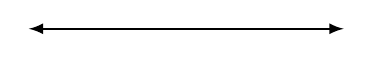
\begin{tikzpicture} \centering  \draw[latex-latex,thick](-0.5,0)--(3.5,0); \end{tikzpicture}\\
\bottomrule
\end{tabular}
\end{table}



\جزوحصہء{عدم مساوات کا حل}
\عددی{x} پر مبنی عدم مساوات کو حل کرتے ہوئے اعداد کا وقفہ یا وقفے تلاش کرنے کو عدم مساوات کا حل کہتے ہیں۔

%=====================
\ابتدا{مثال}\شناخت{مثال_ابتدا_عدم_مساوات_الف}
\begin{multicols}{3}
\begin{enumerate}[1)]
\item
 $2x-4<x+1$
\item
$-\tfrac{x}{3}<x-1$
\item
$\tfrac{2}{x-1}\ge 4$
\end{enumerate}
\end{multicols}
حل:
\begin{enumerate}[1)]
\item
\begin{align*}
2x-4&<x+1&&\\
2x&<x+5&&\text{\RL{دونوں ہاتھ $4$ جمع کریں}}\\
x&<5&& \text{\RL{دونوں ہاتھ سے $x$ منفی کریں}}
\end{align*}
%
\begin{center}
\begin{tikzpicture}
\centering
\draw[-latex](-0.5,0)--(3.5,0)node[right]{$x$};
\draw[thick] (-0.5,0)--(3,0);
\draw(3,0)node[ocirc]{}node[below]{$5$}--++(0,0.1);
\end{tikzpicture}
\end{center}
حل سلسلہ وقفہ \عددی{(-\infty,5)} ہے۔\\
\item
\begin{align*}
-\frac{x}{3}&<x-1\\
-x&<3x-3&&\text{\RL{دونوں ہاتھ کو $3$ سے ضرب دیں}}\\
0&<4x-3&&\text{\RL{دونوں ہاتھ کے ساتھ $x$ جمع کریں}}\\
3&<4x&&\text{\RL{دونوں ہاتھ کے ساتھ $3$ جمع کریں}}\\
\frac{3}{4}&<x&&\text{\RL{دونوں ہاتھ کو $3$ سے تقسیم کریں}}
\end{align*}
%
\begin{center}
\begin{tikzpicture}
\centering
\draw[-latex](-0.5,0)--(3.5,0)node[right]{$x$};
\draw[thick,-latex] (2,0)--(3.5,0);
\draw(2,0)node[ocirc]{}node[below]{$\tfrac{3}{4}$}--++(0,0.1);
\end{tikzpicture}
\end{center}
وقفہ \عددی{(\tfrac{3}{4},\infty)} حل سلسلہ ہے۔\\
\item
عدم مساوات \عددی{\tfrac{2}{x-1}\ge 4} صرف \عددی{x>1} کی صورت میں درست ہو گا چونکہ \عددی{x<1} کی صورت میں بایاں ہاتھ منفی ہو گا اور \عددی{x=1} پر بایاں ہاتھ غیر متعین ہے۔عدم مساوات کے دونوں ہاتھ کو \عددی{x-1} سے ضرب دیتے ہوئے عدم مساوات برقرار رہتا ہے۔
\begin{align*}
\frac{2}{x-1}&\ge 4\\
2&\ge 4x-4&&\text{\RL{دونوں ہاتھ کو $x-1$ سے ضرب دیں}}\\
6&\ge 4x&&\text{\RL{دونوں ہاتھ کے ساتھ $4$ جمع کریں}}\\
\frac{3}{2}&\ge x&&\text{\RL{دونوں ہاتھ کو $4$ سے تقسیم کریں}}
\end{align*}
%
\begin{center}
\begin{tikzpicture}
\draw[-latex](-0.5,0)--(3.5,0)node[right]{$x$};
\draw[thick] (2,0)--(2.5,0);
\draw(2.5,0)node[circ]{}node[below]{$\tfrac{3}{2}$}--++(0,0.1);
\draw(2,0)node[ocirc]{}node[below]{$1$}--++(0,0.1);
\end{tikzpicture}
\end{center}
حل سلسلہ نصف کھلا وقفہ \عددی{(1,\tfrac{3}{2}]} ہے۔
\end{enumerate}
\انتہا{مثال}
%=========================
\جزوحصہء{مطلق قیمت}
عدد \عددی{x} کی \اصطلاح{مطلق قیمت}\فرہنگ{مطلق قیمت}\حاشیہب{absolute value}\فرہنگ{absolute value} جس کو \عددی{\abs{x}} سے ظاہر کیا جاتا ہے کہ تعریف درج ذیل ہے۔
\begin{align*}
\abs{x}=
\begin{cases}
\phantom{-}x&x\ge 0\\
-x&x<0
\end{cases}
\end{align*}

%======================
\ابتدا{مثال}
$\abs{0.88}=0.88,\quad \abs{0}=0,\quad \abs{-13}=-(-13)=13,\quad \abs{-\abs{a}}=\abs{a}$
\انتہا{مثال}
%=========================

دھیان رہے کہ ہر حقیقی عدد کی مطلق قیمت غیر منفی \عددی{\abs{x}\ge } ہو گی اور صرف \عددی{x=0} کی صورت میں \عددی{\abs{x}=0} ہو گا۔چونکہ \عددی{a} کی غیر منفی  جذر کو \عددی{\sqrt{a}} سے ظاہر کیا جاتا ہے لہٰذا \عددی{\abs{x}} کی متبادل تعریف درج ذیل لی جا سکتی ہے۔
\begin{align*}
\abs{x}=\sqrt{x^2}
\end{align*} 
آپ \عددی{\sqrt{a^2}=\abs{a}} لکھ سکتے ہیں جبکہ \عددی{\sqrt{a^2}=a} صرف مثبت \عددی{a} کی صورت میں درست ہو گا۔ 

جیومیٹریائی طور پر حقیقی خط پر مبدا \عددی{0} سے \عددی{x} تک فاصلے کو \عددی{\abs{x}} ظاہر کرتی ہے۔زیادہ عمومی طور پر (شکل \حوالہ{شکل_ابتدائی_مطلق_جیومیٹریائی_مطلب}) 
\begin{align*}
\abs{x-y}=\text{\RL{$\,x\,$ اور $\,y\,$ کے بیچ فاصلہ}}
\end{align*}
ہو گا۔
\begin{figure}
\centering
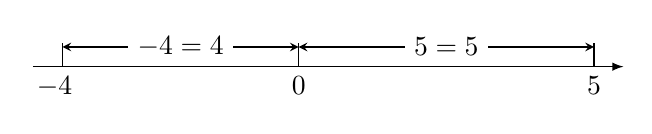
\begin{tikzpicture}[x=0.75cm]
\draw[stealth-stealth] (-4,0.25)--(0,0.25)node[pos=0.5,fill=white]{$\abs{-4}=4$};
\draw[stealth-stealth] (0,0.25)--(5,0.25)node[pos=0.5,fill=white]{$\abs{5}=5$};
\draw[-latex](-4.5,0)--(5.5,0);
\draw(-4,0)node[below,xshift={-1mm}]{$-4$}--++(0,0.3);
\draw(0,0)node[below]{$0$}--++(0,0.3);
\draw(5,0)node[below]{$5$}--++(0,0.3);
\end{tikzpicture}
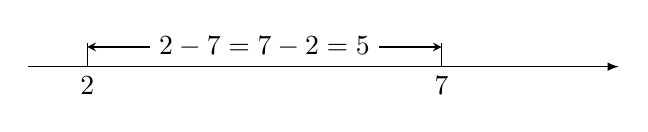
\begin{tikzpicture}[x=0.75cm]
\draw[stealth-stealth](1,0.25)--(7,0.25)node[pos=0.5,fill=white]{$\abs{2-7}=\abs{7-2}=5$};
\draw[-latex](0,0)--(10,0);
\draw(1,0)node[below]{$2$}--++(0,0.3);
\draw(7,0)node[below]{$7$}--++(0,0.3);
\end{tikzpicture}
\caption{مطلق قیمت حقیقی خط پر دو نقطوں کے بیچ فاصلہ دیتا ہے۔}
\label{شکل_ابتدائی_مطلق_جیومیٹریائی_مطلب}
\end{figure}
مطلق قیمت کے درج ذیل خواص پائے جاتے ہیں۔

مطلق قیمت کے خواص درج ذیل ہیں۔
\begin{enumerate}[1.]
\item{$\abs{-a}=\abs{a}$}\quad
کسی بھی عدد اور نفی عدد  کی مطلق قیمتیں ایک جیسی ہوں گی۔
\item{$\abs{ab}=\abs{a}\abs{b}$}\quad
حاصل ضرب کی مطلق قیمت، مطلق قیمتوں کا حاصل ضرب ہو گا۔
\item{$\abs{\frac{a}{b}}=\frac{\abs{a}}{\abs{b}}$}\quad
حاصل تقسیم کی مطلق قیمت، مطلق قیمتوں کا حاصل تقسیم ہو گا۔
\item{$\abs{a+b}\le \abs{a}+\abs{b}$}\quad
دو اعداد کے مجموعہ کی مطلق قیمت دونوں کے مطلق قیمتوں کے مجموعہ سے کم یا اس کے برابر ہو گی۔اس کو \اصطلاح{تکونی عدم مساوات}\فرہنگ{تکونی عدم مساوات} کہتے ہیں۔
\end{enumerate}


اگر \عددی{a} اور \عددی{b} کی علامتیں مختلف ہوں تب \عددی{\abs{a+b}} کی قیمت \عددی{\abs{a}+\abs{b}} کی قیمت سے کم ہو گی۔اس کے علاوہ ہر صورت \عددی{\abs{a+b}=\abs{a}+\abs{b}} ہو گا۔

\ابتدا{مثال}
\begin{align*}
\abs{-2+6}&=\abs{4}=4<\abs{-2}+\abs{6}=8\\
\abs{2+6}&=\abs{8}=\abs{2}+\abs{6}\\
\abs{-2-6}&=\abs{-8}=8=\abs{-2}+\abs{-6}
\end{align*}
\انتہا{مثال}
%============================
مطلق کی علامت قوسین کی طرح کردار ادا کرتی ہے۔مطلق کی علامت کے اندر جمع، منفی وغیرہ مکمل کرنے کے بعد مطلق قیمت حاصل کی جاتی ہے۔

\ابتدا{مثال} 
مساوات \عددی{\abs{2x-1}=11} کو حل کریں۔\\
حل:\quad
اس مساوات کے تحت \عددی{2x-1=\mp 11} ہو سکتا ہے لہٰذا اس کے دو ممکن جوابات ہیں جو مطلق کی علامت کے بغیر دو مساوات سے حاصل کی جاتی ہیں۔
\begin{gather*}
\begin{aligned}
2x-1&=11\\
2x&=12\\
x&=6
\end{aligned}\quad\quad
\begin{aligned}
2x-1&=-11\\
2x&=-10\\
x&=-5
\end{aligned}
\end{gather*}
یوں \عددی{\abs{2x-1}=11} کا درکار حل \عددی{x=6} اور \عددی{x=-5}  ہے۔
\انتہا{مثال}
%====================

\جزوحصہء{مطلق قیمت والے عدم مساوات}
عدم مساوات \عددی{\abs{a}<D} کہتی ہے کہ مبدا \عددی{0} سے \عددی{a} تک فاصلہ \عددی{D} سے کم ہے۔یوں \عددی{D} اور \عددی{-D} کے بیچ \عددی{a} پایا جائے گا۔

\موٹا{مطلق قیمتیں اور وقفے}\quad 
اگر \عددی{D} کوئی مثبت عدد ہو، تب
\begin{align}
\abs{a}&<D \iff -D<a<D\label{مساوات_ابتدائی_عدم_مساوات_الف}\\
\abs{a}&\le D \iff -D\le a\le D\label{مساوات_ابتدائی_عدم_مساوات_ب}
\end{align}


\ابتدا{مثال}
عدم مساوات \عددی{\abs{x-3}<7} کو حل کریں  اور  حل سلسلہ کو حقیقی خط پر ترسیم کریں۔\\
حل:\quad
\begin{align*}
\abs{x-3}&<7\\
-7<x-3&<7 && \text{\RL{مساوات \حوالہ{مساوات_ابتدائی_عدم_مساوات_الف}}}\\
-7+3<x&<7+3&&\text{\RL{دونوں حصوں کے ساتھ $3$ جمع کریں}}\\
-4<x<&10
\end{align*}
حل سلسلہ کھلا وقفہ \عددی{(-4,10)} ہے۔
\begin{center}
\begin{tikzpicture}
\draw[stealth-stealth](0,0.25)--(2,0.25)node[pos=0.5,fill=white]{$7$};
\draw[stealth-stealth](2,0.25)--(4,0.25)node[pos=0.5,fill=white]{$7$};
\draw[-latex](-0.5,0)--(5,0)node[right]{$x$};
\draw[thick](0,0)node[ocirc]{}node[below]{$-4$}--(4,0)node[ocirc]{}node[below]{$10$};
\draw(2,0)node[below]{$3$}--++(0,0.1);
\end{tikzpicture}
\end{center}
\انتہا{مثال}
%===================
\ابتدا{مثال}
عدم مساوات \عددی{\abs{3-\tfrac{2}{x}}<1} کو حل کریں۔\\
حل:\quad
\begin{align*}
\abs{3-\frac{2}{x}}<1 \iff -1&<3-\frac{2}{x}<1 &&\text{\RL{مساوات \حوالہ{مساوات_ابتدائی_عدم_مساوات_الف}}}\\
-4&<-\frac{2}{x}<-2 && \text{\RL{$3$ منفی کریں}}\\
2&>\frac{1}{x}>1 && \text{\RL{$-\tfrac{1}{2}$ سے ضرب دیں}}\\
\frac{1}{2}&<x<1&&\text{\RL{معکوس لیں}}
\end{align*}

اس مثال میں عدم مساوات پر مختلف حسابی اعمال کا اطلاق کیا گیا۔آپ نے دیکھا کہ منفی عدد سے ضرب دینے سے عدم مساوات الٹ ہو جاتی ہے۔اسی طرح اگر دونوں ہاتھ مثبت ہوں تب  معکوس لینے سے عدم مساوات الٹ ہوتی ہے۔ اصل عدم مساوات اس صورت مطمئن ہو گی جب \عددی{\tfrac{1}{2}<x<1} ہو۔حل سلسلہ کھلا وقفہ \عددی{(\tfrac{1}{2},1)} ہے۔
\انتہا{مثال}
%======================
\ابتدا{مثال}
درج ذیل عدم مساوات حل کریں۔حل سلسلہ کو ترسیم  کریں۔
\begin{align*}
(\text{الف})\quad \abs{2x-5}&\le1&& (\text{ب})\quad \abs{2x-5}\ge 1
\end{align*} 
حل:\quad (الف)
\begin{align*}
\abs{2x-5}&\le 1\\
-1\le 2x-5&\le1&&\text{\RL{مساوات \حوالہ{مساوات_ابتدائی_عدم_مساوات_ب}}}\\
4\le 2x&\le 6&&\text{\RL{جمع $5$}}\\
2\le x&\le 3&&\text{\RL{تقسیم $2$}}
\end{align*}
حل سلسلہ بند وقفہ \عددی{[2,3]} ہے۔
\begin{center}
\begin{tikzpicture}
\draw[-latex] (-0.5,0)--(4.5,0)node[right]{$x$};
\draw[thick] (1,0)node[circ]{}node[below]{$2$}--(3,0)node[circ]{}node[below]{$3$};
\end{tikzpicture}
\end{center}
(ب)\quad 
\begin{align*}
\begin{array}{c|c}
\multicolumn{2}{c}{\abs{2x-5}\ge 1}\\
\\
2x-5\ge 1&-(2x-5)\ge 1\\
2x\ge 6&2x-5\le -1\\
x\ge 3&2x\le 4\\
&x\le 2
\end{array}
\end{align*}
حل سلسلہ 
$(-\infty,2] \cup [3,\infty)$
 ہے۔
\begin{center}
\begin{tikzpicture}
\draw[-latex] (-0.5,0)--(4.5,0)node[right]{$x$};
\draw[thick] (1,0)node[circ]{}node[below]{$2$}--(-0.5,0);
\draw[thick](3,0)node[circ]{}node[below]{$3$}--(4.5,0);
\end{tikzpicture}
\end{center}
\انتہا{مثال}
%=======================
درج بالا مثال کے دوسرے حل سلسلہ میں وقفوں کی \اصطلاح{اشتراک}\فرہنگ{اشتراک}\حاشیہب{union}\فرہنگ{union} کی علامت \عددی{\cup} استعمال کی گئی ہے۔دو سلسلوں کی اشتراک میں ایک عدد اس صورت پایا جاتا ہے جب یہ عدد کسی ایک یا دونوں سلسلوں میں پایا جاتا ہو۔اسی طرح ہم \اصطلاح{تقاطع}\فرہنگ{تقاطع}\حاشیہب{intersection}\فرہنگ{intersection} کی علامت \عددی{\cap} بھی استعمال کرتے ہیں۔دو سلسلوں کی تقاطع میں ایک عدد اس صورت پایا جاتا ہے جب یہ عدد دونوں سلسلوں میں پایا جاتا ہو۔مثال کے طور پر 
$[1,3)\cap[2,4]=[2,3)$
ہو گا۔

%==================
\حصہء{سوالات}
%======================
\موٹا{اعشاری روپ}\\
\ابتدا{سوال}
عدد \عددی{\tfrac{1}{9}} کو دہراتے ہندسوں کی روپ میں لکھیں جہاں دہراتے ہندسوں کے اوپر لکیر کھینچی گئی ہو۔اسی طرح \عددی{\tfrac{2}{9}}، \عددی{\tfrac{3}{9}} اور \عددی{\tfrac{8}{9}} کو بھی اعشاری روپ میں لکھیں۔\\
جواب:\quad
$0.\overline{1}, 0.\overline{2},0.\overline{3},0.\overline{8}$
\انتہا{سوال}
%====================
\ابتدا{سوال}
\عددی{\tfrac{1}{11}} کو اعشاری روپ میں لکھیں۔دہراتے ہندسوں کے اوپر لکیر کھینچیں۔\عددی{\tfrac{2}{11}}، \عددی{\tfrac{3}{11}} اور \عددی{\tfrac{9}{11}} کو بھی اعشاری روپ میں لکھیں۔
\انتہا{سوال}
%=====================
\موٹا{عدم مساوات}\\
\ابتدا{سوال}
اگر \عددی{2<x<6} ہو تب درج ذیل میں کون سے حسابی فقرے \عددی{x} کے لئے لازماً درست ہیں اور کون سے ضروری نہیں کہ درست ہوں۔
\begin{multicols}{3}
\begin{enumerate}[a]
\item
$0<x<4 $
\item
$0<x-2<4$
\item
$1<\tfrac{x}{2}<3$
\item
$\tfrac{1}{6}<\tfrac{1}{x}<\tfrac{1}{2}$
\item
$1<\tfrac{6}{x}<3$
\item
$\abs{x-4}<2$
\item
$-6<-x<2$
\item
$ -6<-x<-2$
\end{enumerate}
\end{multicols}

\انتہا{سوال}
%===================
\ابتدا{سوال}
اگر \عددی{-1<y-5<1} ہو تب درج ذیل  میں سے کون سے حسابی فقرے \عددی{ y} کے لئے لازماً درست ہیں اور کون سے ضروری نہیں کہ درست ہوں۔
\begin{multicols}{3}
\begin{enumerate}[a]
\item
$4<y<6$
\item
$-6<y<-4$
\item
$y>4$
\item
$y<6$
\item
$0<y-4<2$
\item
$2<\frac{y}{2}<3$
\item
$\frac{1}{6}<\frac{1}{y}<\frac{1}{4}$
\item
$\abs{y-5}<1$
\end{enumerate}
\end{multicols} 
\انتہا{سوال}
%====================
عدم مساوات حل کرتے ہوئے حل سلسلہ کو ترسیم کریں۔
\begin{multicols}{2}
\begin{enumerate}[]
\item
\ابتدا{سوال}
$-2x>4$\\
جواب:\quad 
$x<-2$
\انتہا{سوال}
\item
\ابتدا{سوال}
$8-3x\ge 5$
\انتہا{سوال}
\item
\ابتدا{سوال}
$5x-3\le 7-3x$\\
جواب:\quad
$x\le \tfrac{5}{4}$
\انتہا{سوال}
\item
\ابتدا{سوال}
$3(2-x)>2(3+x)$
\انتہا{سوال}
\item
\ابتدا{سوال}
$2x-\frac{1}{2}\ge 7x+\frac{7}{6}$\\
جواب:\quad 
$x\le -\tfrac{1}{3}$
\انتہا{سوال}
\item
\ابتدا{سوال}
$\frac{6-x}{4}<\frac{3x-4}{2}$
\انتہا{سوال}
\item
\ابتدا{سوال}
$\frac{4}{5}(x-2)<\frac{1}{3}(x-6)$\\
جواب:\quad
$x<-\tfrac{6}{7}$
\انتہا{سوال}
\item
\ابتدا{سوال}
$-\frac{x+5}{2}\le \frac{12+3x}{4}$
\انتہا{سوال}
\end{enumerate}
\end{multicols}

\موٹا{مطلق قیمت}\\
سوال \حوالہ{سوال_ابتدا_مطلق_الف} تا سوال \حوالہ{سوال_ابتدا_مطلق_ب} میں دیے مساوات حل کریں۔
\begin{multicols}{2}
\begin{enumerate}[]
\item
\ابتدا{سوال}\شناخت{سوال_ابتدا_مطلق_الف}
$\abs{y}=3$\\
جواب:\quad
$\mp 3$
\انتہا{سوال}
\item
\ابتدا{سوال}
$\abs{y-3}=7$
\انتہا{سوال}
\item
\ابتدا{سوال}
$\abs{2t+5}=4$\\
جواب:\quad
$-\tfrac{1}{2},\quad -\tfrac{9}{2}$
\انتہا{سوال}
\item
\ابتدا{سوال}
$\abs{1-t}=1$
\انتہا{سوال}
\item
\ابتدا{سوال}
$\abs{8-3s}=\frac{9}{2}$\\
جواب:\quad
$\tfrac{7}{6},\quad \tfrac{25}{6} $
\انتہا{سوال}
\item
\ابتدا{سوال}\شناخت{سوال_ابتدا_مطلق_ب}
$\abs{\frac{s}{2}-1}=1$
\انتہا{سوال}
\end{enumerate}
\end{multicols}

سوال \حوالہ{سوال_ابتدا_عدم_مساوات_الف} تا سوال \حوالہ{سوال_ابتدا_عدم_مساوات_ب} میں دیے عدم مساوات حل کریں۔حل سلسلہ کو وقفوں یا وقفوں کے اشتراک کی صورت میں لکھیں۔حل سلسلہ کو  ترسیم کریں\\
%
\ابتدا{سوال}\شناخت{سوال_ابتدا_عدم_مساوات_الف}
$\abs{x}<2$\\
جواب:\quad
$-2<x<2$
\انتہا{سوال}
%=======================
\ابتدا{سوال}
$\abs{x}\le 2$
\انتہا{سوال}
%======================
\ابتدا{سوال}
$\abs{t-1}\le 3$\\
جواب:\quad
$-2\le t\le 4$
\انتہا{سوال}
%====================
\ابتدا{سوال}
$\abs{t+2}<1$
\انتہا{سوال}
%=====================
\ابتدا{سوال}
$\abs{3y-7}<4$\\
جواب:\quad
$1<y<\tfrac{11}{3}$
\انتہا{سوال}
%====================
\ابتدا{سوال}
$\abs{2y+5}<1$
\انتہا{سوال}
%================
\ابتدا{سوال}
$\abs{\frac{z}{5}-1}\le 1$\\
جواب:\quad
$0\le z\le 10$
\انتہا{سوال}
%=====================
\ابتدا{سوال}
$\abs{\frac{3}{2}z-1}\le 2$
\انتہا{سوال}
%====================
\ابتدا{سوال}
$\abs{3-\frac{1}{x}}<\frac{1}{2}$\\
جواب:\quad
$\tfrac{2}{7}<y<\tfrac{11}{3} \quad \text{یا} \quad \tfrac{10}{35}<x<\tfrac{14}{35}$
\انتہا{سوال}
%==================
\ابتدا{سوال}
$\abs{\frac{2}{x}-4}<3$
\انتہا{سوال}
%===================
\ابتدا{سوال}
$\abs{2s}\ge 4$\\
جواب:\quad
$(-\infty,-2]\cup [2,\infty)$
\انتہا{سوال}
%=================
\ابتدا{سوال}
$\abs{s+3}\ge \frac{1}{2}$
\انتہا{سوال}
%======================
\ابتدا{سوال}
$\abs{1-x}>1$\\
جواب:\quad
$(-\infty,0)\cup (2,\infty)$
\انتہا{سوال}
%==========================
\ابتدا{سوال}
$\abs{2-3x}>5$
\انتہا{سوال}
%==========================
\ابتدا{سوال}
$\abs{\frac{r+1}{2}}\ge 1$\\
جواب:\quad
$(-\infty,-3]\cup [1,\infty)$
\انتہا{سوال}
%===================
\ابتدا{سوال}\شناخت{سوال_ابتدا_عدم_مساوات_ب}
$\abs{\frac{3}{5}r-1}>\frac{2}{5}$
\انتہا{سوال}
%=======================
\موٹا{دو درجی عدم مساوات}\\
سوال \حوالہ{سوال_ابتدا_دو_درجی_عدم_مساوات_الف} تا سوال \حوالہ{سوال_ابتدا_دو_درجی_عدم_مساوات_ب} میں دیے دو درجی عدم مساوات حل کرتے ہوئے حل سلسلہ کو ترسیم کریں اور اس کو وقفوں کی اشتراک کی صورت میں لکھیں۔ جہاں ضرورت ہو وہاں \عددی{\sqrt{a^2}=\abs{a}} کا استعمال کریں۔

\ابتدا{سوال}\شناخت{سوال_ابتدا_دو_درجی_عدم_مساوات_الف}
$x^2<2$\\
جواب\quad
$(-\sqrt{2},\sqrt{2})$
\انتہا{سوال}
%======================
\ابتدا{سوال}
$4\le x^2$
\انتہا{سوال}
%===================
\ابتدا{سوال}
$4<x^2<9$\\
جواب\quad
$(-3,-2)\cup (2,3)$
\انتہا{سوال}
%====================
\ابتدا{سوال}
$\frac{1}{9}<x^2<\frac{1}{4}$
\انتہا{سوال}
%====================
\ابتدا{سوال}
$(x-1)^2<4$\\
جواب\quad
$(-1,3)$
\انتہا{سوال}
%====================
\ابتدا{سوال}
$(x+3)^2<2$
\انتہا{سوال}
%====================
\ابتدا{سوال}
$x^2-x<0$\\
جواب\quad
$(0,1)$
\انتہا{سوال}
%====================
\ابتدا{سوال}\شناخت{سوال_ابتدا_دو_درجی_عدم_مساوات_ب}
$x^2-x-2\ge 0$
\انتہا{سوال}
%====================
\موٹا{نظریہ اور مثالیں}\\

\ابتدا{سوال}
اس غلط فہمی میں مبتلا نہ ہوں کہ \عددی{\abs{-a}=a} ہے۔کس حقیقی عدد \عددی{a} کے لئے ایسا درست ہے اور کس کے لئے یہ درست نہیں ہے۔\\
جواب:\quad
تمام منفی حقیقی اعداد کے لئے یہ غلط ہے جبکہ \عددی{a\ge 0} کے لئے درست ہے۔
\انتہا{سوال}
%====================
\ابتدا{سوال}
مساوات \عددی{\abs{x-1}=1-x} کو حل کریں۔
\انتہا{سوال}
%=======================
\ابتدا{سوال}
\ترچھا{تکونی عدم مساوات کا ثبوت۔} \عددی{\abs{a+b}=(a+b)^2} سے شروع کرتے ہوئے تکونی عدم مساوات کو درج ذیل طریقہ سے ثابت کریں۔
\begin{align*}
\abs{a+b}^2&=(a+b)^2\\
&=a^2+2ab+b^2\\
&\le a^2+2\abs{a}\abs{b}+b^2\\
&\le \abs{a}^2+2\abs{a}\abs{b}+\abs{b}^2\\
&=(\abs{a}+\abs{b})^2\\
\abs{a+b}&\le \abs{a}+\abs{b}
\end{align*}
\انتہا{سوال}
%====================
\ابتدا{سوال}
ثابت کریں کہ کسی بھی اعداد \عددی{a} اور \عددی{b} کے لئے  \عددی{\abs{ab}=\abs{a}\abs{b}} ہو گا۔
\انتہا{سوال}
%===================
\ابتدا{سوال}
اگر \عددی{\abs{x}\le 3} اور \عددی{x>-\tfrac{1}{2}} ہوں تب \عددی{x} کے بارے میں کیا کہا جا سکتا ہے؟\\
جواب:\quad
$-\tfrac{1}{2}<x\le 3$
\انتہا{سوال}
%===================
\ابتدا{سوال}
عدم مساوات \عددی{\abs{x}+\abs{y}\le 1} کو ترسیم کریں۔
\انتہا{سوال}
%====================
\ابتدا{سوال}
(الف) \quad \عددی{f(x)=\tfrac{x}{2}} اور \عددی{g(x)=1+\tfrac{4}{x}} کو ایک جگہ ترسیم کرتے ہوئے \عددی{x} کی وہ قیمتیں تلاش کریں جن پر \عددی{\tfrac{x}{2}>1+\tfrac{4}{x}} ہو گا۔\\
(ب) \quad
ترسیم سے حاصل نتیجہ کو تحلیلی طور پر دوبارہ ثابت کریں۔ \\
جواب:\quad
$(-2,0)\cup (4,\infty)$
\انتہا{سوال}
%====================
\ابتدا{سوال}
(الف) \quad
تفاعل \عددی{f(x)=\tfrac{3}{x-1}} اور \عددی{g(x)=\tfrac{2}{x+1}} کو ایک جگہ ترسیم کرتے ہوئے \عددی{x} کی وہ قیمتیں تلاش کریں جن پر \عددی{\tfrac{3}{x-1}<\tfrac{2}{x+1}} ہو گا۔\\
(ب)\quad
ترسیم سے حاصل نتیجہ کو تحلیلی طور پر ثابت کریں۔
\انتہا{سوال}
%===================

\حصہ{محدد، خطوط اور بڑھوتری}
اس حصہ میں محدد اور خطوط پر نظرثانی کی جائے گی اور اضافے کی تصور پر بھی غور کیا جائے گا۔

\جزوحصہء{مستوی میں کارتیسی محدد} 
مستوی میں دو حقیقی قائمہ خطوط شکل \حوالہ{شکل_ابتدا_کارتیسی_محدد} میں دکھائی گئی ہیں جو ایک دوسرے کو \عددی{0} پر قطع کرتی ہیں۔ان خطوط کو مستوی میں \اصطلاح{محددی محور}\فرہنگ{محددی محور}\حاشیہب{coordinate axis}\فرہنگ{coordinate!axis} کہتے ہیں۔افقی \عددی{x} محور پر اعداد کو \عددی{x} سے ظاہر کیا جاتا ہے جو دائیں رخ بڑھتے ہیں۔انتصابی \عددی{y} محور پر اعداد کو \عددی{y} سے ظاہر کیا جاتا ہے اور یہ اعداد اوپر رخ بڑھتے ہیں۔وہ نقطہ جس پر \عددی{x} اور \عددی{y} دونوں \عددی{0} ہوں محددی نظام کا \اصطلاح{مبدا}\فرہنگ{مبدا}\حاشیہب{origin}\فرہنگ{origin}  کہلاتا ہے جس کو عموماً  حرف \عددی{M} سے ظاہر کیا جاتا ہے۔
\begin{figure}
\centering
\begin{subfigure}{0.5\textwidth}
\centering
\begin{tikzpicture}
\draw[-latex](-1.5,0)--(3.2,0)node[right]{$x$};
\draw[-latex](0,-2.2)--(0,3.5)node[above]{$y$};
\foreach \x in {1,2}{\draw(\x,0)node[below]{$\x$}--++(0,0.1);}
\draw(-1,0)node[below,xshift={(-1mm)}]{$-1$}--++(0,0.1);
\foreach \y in {-2,-1,1,2,3}{\draw(0,\y)node[left]{$\y$}--++(0.1,0);}
\draw(0,0)node[circ]{}node[below left]{$0$};
\draw(-0.1,-1.4)--++(-160:1)node[left]{\RL{منفی $\,y\,$ محور}};
\draw(-0.1,1.4)--++(145:1)node[left]{\RL{مثبت $\,y\,$ محور}};
\draw(0.1,0.1)--++(30:1)node[right]{مبدا};
\draw(-0.6,0.1)--++(135:1)node[above]{\RL{منفی $\,x\,$ محور}};
\draw(1.4,-0.1)--++(-45:1)node[below]{\RL{مثبت $\,x\,$ محور}};
\draw[dashed](0,2.6)node[left]{$b$}coordinate(kA)--++(2.5,0)coordinate(kB)node[circ]{}node[right]{$P(a,b)$}--++(0,-2.6)node[below]{$a$}coordinate(kC);
\RightAngle{(kB)}{(kA)}{(0,0)};
\RightAngle{(kB)}{(kC)}{(0,0)};
\end{tikzpicture}
\end{subfigure}%
\begin{subfigure}{0.5\textwidth}
\centering
\begin{tikzpicture}
\draw[-latex](-2.5,0)--(2.5,0)node[right]{$x$};
\draw[-latex](0,-2.2)--(0,3.5)node[above]{$y$};
\foreach \x in {1,2}{\draw(\x,0)node[below]{$\x$}--++(0,0.1)node[above,font=\footnotesize]{$(\x,0)$};}
\foreach \x in {-1,-2}\draw(\x,0)node[below,xshift={(-1mm)}]{$\x$}--++(0,0.1);
\draw(-2,0)++(0,0.1)node[above,font=\footnotesize]{$(-2,0)$};
\foreach \y in {-2,-1,1,2,3}{\draw(0,\y)node[left]{$\y$}--++(0.1,0)node[right,font=\footnotesize]{$(0,\y)$};}
\draw(0,0)node[circ]{}node[below left]{$0$};
\draw(-0.1,0.1)--++(135:0.5)node[left,font=\footnotesize]{(0,0)};
\draw(2,2)node[above]{\RL{ربع اول}}node[below,font=\footnotesize]{$(+,+)$};
\draw(-1.75,2)node[above]{\RL{ربع دوم}}node[below,font=\footnotesize]{$(-,+)$};
\draw(-1.75,-1.5)node[above]{\RL{ربع سوم}}node[below,font=\footnotesize]{$(-,-)$};
\draw(2,-1.5)node[above]{\RL{ربع چہارم}}node[below,font=\footnotesize]{$(+,-)$};
\end{tikzpicture}
\end{subfigure}%
\caption{کارتیسی محدد}
\label{شکل_ابتدا_کارتیسی_محدد}
\end{figure}

مستوی میں نقطہ \عددی{P} سے دونوں محور پر قائمہ خطوط کھینچے جا سکتے ہیں۔اگر \عددی{P} سے \عددی{x} محور پر قائمہ خط \عددی{x} محور کو \عددی{a} پر قطع کرتا ہو تب \عددی{P} کا \اصطلاح{\عددی{x} محدد}\فرہنگ{محدد!ایکس}\حاشیہب{x-coordinate}\فرہنگ{coordinate!x} \عددی{a} ہو گا۔اسی طرح اگر \عددی{P} سے \عددی{y} محور پر قائمہ خط \عددی{y} محور کو \عددی{b} پر قطع کرتا ہو تب \عددی{P} کا \اصطلاح{\عددی{y} محدد}\فرہنگ{محدد!وائے}\حاشیہب{y-coordinate}\فرہنگ{coordinate!y} \عددی{b} ہو گا۔  مرتب جوڑی \عددی{(a,b)} کو نقطے کی \اصطلاح{محددی جوڑی}\فرہنگ{محددی جوڑی}\حاشیہب{coordinate pair}\فرہنگ{coordinate!pair} کہتے ہیں۔\عددی{x} محور پر ہر محددی جوڑی کا \عددی{y} محدد \عددی{0} ہو گا جبکہ \عددی{y} محور پر ہر محددی جوڑی کا \عددی{x} محدد \عددی{0} ہو گا۔محددی نظام کا مبدا نقطہ \عددی{(0,0)} ہے۔ 

محور \عددی{x}  کو مبدا دو حصوں میں تقسیم کرتا ہے۔مبدا کے دائیں جانب \اصطلاح{مثبت \عددی{x} محور}\فرہنگ{محور!مثبت ایکس}\حاشیہب{positive x-axis}\فرہنگ{axis!positive-x} اور مبدا کے بائیں جانب \اصطلاح{منفی \عددی{x} محور}\فرہنگ{محور!منفی ایکس}\حاشیہب{negative x-axis}\فرہنگ{axis!negative-x} پایا جاتا ہے۔ اسی طرح مبدا \عددی{y} محور کو بھی \اصطلاح{مثبت \عددی{y} محور} اور \اصطلاح{منفی \عددی{y} محور} میں تقسیم کرتا ہے۔محدد مستوی کو چار \اصطلاح{ربعات}\فرہنگ{ربعات}\حاشیہب{quadrants}\فرہنگ{quadrants} میں تقسیم کرتے ہیں جنہیں (گھڑی کی الٹ رخ چلتے ہوئے) ربع اول، ربع دوم، ربع سوم اور ربع چہارم کہتے ہیں (شکل \حوالہ{شکل_ابتدا_کارتیسی_محدد})۔

\جزوحصہء{پیما}
ایسا ترسیم، مثلاً رفتار بالمقابل وقت، جس کے دو متغیرات کی اکائیاں مختلف ہوں میں دونوں محور پر اکائی متغیر کو ایک جیسا رکھنے کی کوئی ضرورت نہیں ہوتی ہے۔یوں رفتار بالمقابل وقت کی ترسیم میں محور وقت پر ایک سنٹی میٹر کا فاصلہ ایک سیکنڈ کو ظاہر کر سکتا ہے جبکہ رفتار کی محور پر ایک سنٹی میٹر کا فاصلہ \عددی{\SI{25}{\meter\per\second}} کی رفتار کو ظاہر کر سکتی ہے۔

اس کے برعکس ایسے متغیرات کی ترسیم جو غیر طبعی پیمائشوں کو ظاہر کرتی ہو یا ایسے ترسیم جن میں اشکال کا معائنہ کرنا مقصد ہو، ہم دونوں محور کی \اصطلاح{تناسب پہلو}\فرہنگ{تناسب پہلو}\حاشیہب{aspect ratio}\فرہنگ{aspect ratio} ایک جیسے رکھتے ہیں لہٰذا دونوں محور پر پیمانہ ایک جیسا ہو گا۔

\جزوحصہء{بڑھوتری اور فاصلہ}
ایک نقطہ سے دوسرے نقطے تک حرکت کرنے سے محدد میں کل تبدیلی کو \اصطلاح{بڑھوتری}\فرہنگ{بڑھوتری}\حاشیہب{increments}\فرہنگ{increments} کہتے ہیں۔ اختتامی محدد سے ابتدائی محدد منفی کرنے سے بڑھوتری حاصل ہو گی۔

\ابتدا{مثال}
نقطہ \عددی{A(4,-3)} سے نقطہ \عددی{B(2,5)} منتقل ہونے سے  بڑھوتری \عددی{x} اور بڑھوتری \عددی{y} درج ذیل ہوں گی (شکل \حوالہ{شکل_ابتدائی_بڑھوتری})۔
\begin{align*}
\Delta x=2-4=2,\quad \Delta y=5-(-3)=8
\end{align*}
\انتہا{مثال}
%
\begin{figure}
\centering
\begin{tikzpicture}[y={0.5cm}]
\draw[-latex](0,0)node[left]{$0$}--(6.5,0)node[right]{$x$};
\draw[-latex](0,-3.2)--(0,6.5)node[above]{$y$};
\foreach \x in {1,2,3,4,5,6}{\draw(\x,0)node[below]{$\x$}--++(0,0.1);}
\foreach \y in {-3,-2,-1,1,2,3,4,5,6}{\draw(0,\y)node[left]{$\y$}--++(0.1,0);}
\draw[->-=0.5](4,-3)node[circ]{}node[right]{$A(4,-3)$} to [out=90,in=-70] (2,5)node[right]{$B(2,5)$}node[circ]{};
\draw[dashed](2,-3)node[circ]{}node[below]{$(2,-3)$}--(4,-3)node[above,pos=0.5]{$\Delta x=-2$};
\draw[dashed](2,-3)--(2,5)node[left,pos=0.5]{$\Delta y=8$};
\draw[->-=0.5](5,6)node[right]{$C(5,6)$}node[circ]{}--(5,1)node[circ]{}node[right]{$D(5,1)$}node[pos=0.5,right]{$\substack{\Delta x=0 \hfill\\  \Delta y=-5}$};
\end{tikzpicture}
\caption{محددی بڑھوتری مثبت، منفی اور صفر ہو سکتی ہیں}
\label{شکل_ابتدائی_بڑھوتری}
\end{figure}
%===================
\ابتدا{تعریف}
اگر متغیر \عددی{x} کی ابتدائی قیمت \عددی{x_1} اور اختتامی قیمت \عددی{x_2} ہو تب \عددی{x} کی بڑھوتری درج ذیل ہو گی۔
\begin{align*}
\Delta x=x_2-x_1
\end{align*}
\انتہا{تعریف}
%=========================
\ابتدا{مثال}
شکل \حوالہ{شکل_ابتدائی_بڑھوتری} میں ابتدائی نقطہ \عددی{C(5,6)} اور اختتامی نقطہ \عددی{D(5,1)} ہے۔بڑھوتری تلاش کریں۔\\
حل:\quad
$\Delta x=5-5=0,\quad \Delta y=1-6=-5$
\انتہا{مثال}
%========================

مستوی میں نقطوں کے بیچ فاصلہ مسئلہ فیثاغورث کی مدد سے حاصل کیا جاتا ہے۔

\موٹا{مستوی میں نقطوں کے بیچ فاصلے کا کلیہ}\quad
نقطہ \عددی{P(x_1,y_1)} اور نقطہ \عددی{Q(x_2,y_2)} کے بیچ فاصلہ درج ذیل ہو گا (شکل \حوالہ{شکل_ابتدائی_نقطوں_کے_بیچ_فاصلہ})۔
\begin{align*}
d=\sqrt{(\Delta x)^2+(\Delta y)^2}=\sqrt{(x_2-x_1)^2+(y_2-y_1)^2}
\end{align*}

%==========================
\begin{figure}
\centering
\begin{tikzpicture}
\draw[-latex](-0.5,0)--(7,0)node[right]{$x$};
\draw[-latex](0,-0.5)--(0,3)node[above]{$y$};
\draw(3,0.5)node[left]{$P(x_1,y_1)$}--(6,0.5)node[right]{$C(x_2,y_1)$}--(6,2)node[right]{$Q(x_2,y_2)$}--(3,0.5);
\RightAngle{(6,2)}{(6,0.5)}{(3,0.5)};
\draw[thick](3,0)node[below]{$x_1$}--(6,0)node[below]{$x_2$};
\draw(3,0)--++(0,0.1);
\draw(6,0)--++(0,0.1);
\draw[thick](0,0.5)--(0,2);
\draw(0,0.5)node[left]{$y_1$}--++(0.1,0);
\draw(0,2)node[left]{$y_2$}--++(0.1,0);
\draw(2.5,2.5)node[font=\footnotesize]{$\begin{aligned}d&=\sqrt{\abs{x_2-x_1}^2+\abs{y_2-y_1}^2}\\  &=\sqrt{(x_2-x_1)^2+(y_2-y_1)^2}\end{aligned}$};
\draw($(3,0.5)!0.5!(6,2)$)++(-0.1,0.1) to [out=135,in=-90]++(-1.5,0.5);
\end{tikzpicture}
\caption{دو نقطوں کے بیچ فاصلہ (مسئلہ فیثاغورث)}
\label{شکل_ابتدائی_نقطوں_کے_بیچ_فاصلہ}
\end{figure}

\ابتدا{مثال}
(الف)\quad
\عددی{P(-1,2)} اور \عددی{Q(3,4)} کے بیچ فاصلہ درج ذیل ہو گا۔
\begin{align*}
\sqrt{(3-(-1))^2+(4-2)^2}=\sqrt{(4)^2+(2)^2}\sqrt{20}=\sqrt{4\cdot 5}=2\sqrt{5}
\end{align*} 
(ب)\quad
مبدا سے \عددی{P(x,y)} تک فاصلہ درج ذیل ہو گا۔
\begin{align*}
\sqrt{(x-0)^2+(y-0)^2}=\sqrt{x^2+y^2}
\end{align*}
\انتہا{مثال}
%====================

\جزوحصہء{ترسیم}
متغیرات \عددی{x} اور \عددی{y} پر مبنی مساوات یا عدم مساوات کی ترسیم سے مراد ان تمام نقطوں \عددی{P(x,y)} کا سلسلہ ہے جو اس مساوات یا عدم مساوات کو مطمئن کرتے ہوں۔

\ابتدا{مثال}\شناخت{مثال_ابتدائی_مساوات_عدم_مساوات_ترسیم}دائرے جن کا مرکز مبدا پر ہو\\
(الف)\quad
\عددی{a>0} کی صورت میں مساوات \عددی{x^2+y^2=a^2} ان تمام نقطوں \عددی{P(x,y)} کو ظاہر کرتی ہے جن کا مبدا سے فاصل \عددی{\sqrt{x^2+y^2}=\sqrt{a^2}=a} ہو۔یہ نقطے مبدا کے گرد رداس \عددی{a} کے دائرے پر پائے جاتے ہیں۔یہ دائرہ مساوات \عددی{x^2+y^2=a^2} کی ترسیم ہے (شکل \حوالہ{شکل_مثال_ابتدائی_مساوات_عدم_مساوات_ترسیم})۔ \\
(ب)\quad
عدم مساوات \عددی{x^2+y^2\le a^2} کو مطمئن کرتے ہوئے نقطوں \عددی{(x,y)} کا مبدا سے فاصل \عددی{\le a} ہے۔یوں مبدا کو مرکز بناتے ہوئے رداس \عددی{a} کا دائرہ اور اس کی اندرون اس عدم مساوات کی ترسیم ہو گی (شکل \حوالہ{شکل_مثال_ابتدائی_مساوات_عدم_مساوات_ترسیم})۔
\begin{figure}
\centering
\begin{subfigure}{0.5\textwidth}
\centering
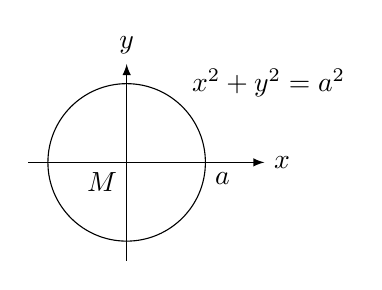
\begin{tikzpicture}
\draw[-latex](-1.25,0)--(1.75,0)node[right]{$x$};
\draw[-latex](0,-1.25)--(0,1.25)node[above]{$y$};
\draw (0,0) circle (1);
\draw(1,0)node[below right]{$a$};
\draw(0,0)node[below left]{$M$};
\draw(45:1)node[above right]{$x^2+y^2=a^2$};
\end{tikzpicture}
\caption{مساوات کی ترسیم}
\end{subfigure}%
\begin{subfigure}{0.5\textwidth}
\centering
\begin{tikzpicture}
\draw[fill=lgray] (0,0) circle (1);
\draw[-latex](-1.25,0)--(1.75,0)node[right]{$x$};
\draw[-latex](0,-1.25)--(0,1.25)node[above]{$y$};
\draw(1,0)node[below right]{$a$};
\draw(0,0)node[below left]{$M$};
\draw(45:1)node[above right]{$x^2+y^2\le a^2$};
\end{tikzpicture}
\caption{عدم مساوات کی ترسیم}
\end{subfigure}%
\caption{مساوات اور عدم مساوات کی ترسیم (مثال \حوالہ{مثال_ابتدائی_مساوات_عدم_مساوات_ترسیم})}
\label{شکل_مثال_ابتدائی_مساوات_عدم_مساوات_ترسیم}
\end{figure}
\انتہا{مثال}
%========================

اکائی رداس کا دائرہ جس کا مرکز مبدا ہو کو \اصطلاح{اکائی دائرہ}\فرہنگ{اکائی دائرہ}\حاشیہب{unit circle}\فرہنگ{unit circle} کہتے ہیں۔

\ابتدا{مثال}\شناخت{مثال_ابتدائی_قطع_مکافی}
مساوات \عددی{y=x^2} پر غور کریں۔\عددی{(0,0)}، \عددی{(1,1)}، \عددی{(-1,1)}، \عددی{(2,4)} اور \عددی{(-2,4)} ایسی چند نقطے ہیں جن کے محدد اس مساوات کو مطمئن کرتے ہیں۔یہ نقطے (اور ایسے تمام باقی نقطے جو اس مساوات کو مطمئن کرتے ہوں) مل کر ہموار منحنی دیتے ہیں جس کو \اصطلاح{قطع مکافی}\فرہنگ{قطع مکافی}\حاشیہب{parabola}\فرہنگ{parabola} کہتے ہیں (شکل \حوالہ{شکل_مثال_ابتدائی_قطع_مکافی})۔
\begin{figure}
\centering
\begin{tikzpicture}
\begin{axis}[small,axis lines*=middle,xlabel={$x$},ylabel={$y$},xlabel style={at={(current axis.right of origin)},anchor=north west}, ylabel style={rotate=-90},ylabel style={at={(current axis.above origin)},anchor=north east},ytick={1,4},yticklabels={$2$,$4$},xmax=2.9]
\addplot[domain=-2.2:2.2]{x^2}node[pos=0.75,right]{$y=x^2$};
\addplot[mark=none] plot coordinates {(0,0)}node[circ]{};
\addplot[mark=none] plot coordinates {(-2,4)}node[circ]{}node[right]{$(-2,4)$};
\addplot[mark=none] plot coordinates {(2,4)}node[circ]{}node[left]{$(2,4)$};
\addplot[mark=none] plot coordinates {(1,1)}node[circ]{}node[right]{$(1,1)$};
\addplot[mark=none] plot coordinates {(-1,1)}node[circ]{}node[left]{$(-1,1)$};
\end{axis}
\end{tikzpicture}
\caption{قطع مکافی (مثال \حوالہ{مثال_ابتدائی_قطع_مکافی})}
\label{شکل_مثال_ابتدائی_قطع_مکافی}
\end{figure}

\انتہا{مثال}
%============================
\جزوحصہء{سیدھے خطوط}
مستوی میں دو نقطوں \عددی{N_1(x_1,y_1)} اور \عددی{N_2(x_2,y_2)} سے یکتا سیدھا خط گزرتا ہے جس کو عموماً خط \عددی{N_1N_2} کہتے ہیں۔ 

مستوی میں کسی بھی غیر انتصابی خط پر ہر دو نقطوں \عددی{N_1(x_1,y_1)} اور \عددی{N_2(x_2,y_2)} کے لئے درج ذیل نسبت
\begin{align*}
m=\frac{\Delta y}{\Delta x}=\frac{y_2-y_1}{x_2-x_1}
\end{align*}
کی قیمت ایک جیسی ہو گی (شکل \حوالہ{شکل_ابتدائی_سیدھا_خط_ڈھلوان})۔
\begin{figure}
\centering
\begin{tikzpicture}
\pgfmathsetmacro{\ang}{30}
\pgfmathsetmacro{\xA}{0.5*cos(\ang)}
\pgfmathsetmacro{\xB}{1.5*cos(\ang)}
\pgfmathsetmacro{\xC}{3*cos(\ang)}
\pgfmathsetmacro{\xD}{4*cos(\ang)}
\pgfmathsetmacro{\yA}{0.5*sin(\ang)}
\pgfmathsetmacro{\yB}{1.5*sin(\ang)}
\pgfmathsetmacro{\yC}{3*sin(\ang)}
\pgfmathsetmacro{\yD}{4*sin(\ang)}
\draw[-latex](-0.5,0)--+(5,0)node[right]{$x$};
\draw[-latex](0,-0.25)--(0,2.5)node[above]{$y$};
\draw(-0.5,0.5)--++(\ang:5)node[above]{$L$};
\draw(-0.5,0.5)++(\ang:0.5)coordinate(kA)node[circ]{}++(\ang:1)coordinate(kB)node[circ]{}++(\ang:1.5)coordinate(kC)node[circ]{}++(\ang:1)coordinate(kD)node[circ]{};
\draw(kA)node[shift={(90+\ang:0.4)}]{$N_1'$};
\draw(kB)node[shift={(90+\ang:0.5)}]{$N_1(x_1,y_1)$};
\draw(kC)node[shift={(90+\ang:0.5)}]{$N_2(x_2,y_2)$};
\draw(kD)node[shift={(90+\ang:0.4)}]{$N_2'$};
\draw(kB)--++(\xC-\xB,0)node[pos=0.5,below]{$\Delta x$}coordinate(kE)node[shift={(0.15,-0.15)}]{$Q$};
\draw(kE)--++(0,\yC-\yB)node[pos=0.5,right]{$\Delta y$};
\draw(kA)--++(\xD-\xA,0)node[pos=0.5,below]{$\Delta x'$}coordinate(kF)node[shift={(0.15,-0.15)}]{$Q'$};
\draw(kF)--++(0,\yD-\yA)node[pos=0.5,right]{$\Delta y'$};
\end{tikzpicture}
\caption{$N_1QN_2$ اور $N_1'Q'N_2'$ متشابہ مثلثات ہیں لہٰذا $\tfrac{\Delta y}{\Delta x}=\tfrac{\Delta y'}{\Delta x'}$ ہو گا}
\label{شکل_ابتدائی_سیدھا_خط_ڈھلوان}
\end{figure}

\ابتدا{تعریف}
درج ذیل شرح
\begin{align*}
m=\frac{\Delta y}{\Delta x}=\frac{y_2-y_1}{x_2-x_1}
\end{align*}
غیر انتصابی خط \عددی{N_1N_2} کی \اصطلاح{ڈھلوان}\فرہنگ{ڈھلوان}\حاشیہب{slope}\فرہنگ{slope} کہلاتی ہے۔
\انتہا{تعریف}
%========================

ڈھلوان ہمیں خط کی چڑھائی یا اترائی دیتی ہے۔مثبت ڈھلوان کے خط پر دائیں رخ چلتے ہوئے چڑھائی نظر آئے گی جبکہ منفی ڈھلوان کے خط پر دائیں رخ چلتے ہوئے اترائی نظر آئے گی۔ڈھلوان کی مطلق قیمت جتنی زیادہ ہو چڑھائی یا اترائی اتنی زیادہ ہو گی۔انتصابی خط کی ڈھلوان کے لئے \عددی{\Delta x=0} ہو گا لہٰذا شرح \عددی{\tfrac{\Delta y}{\Delta x}} غیر معین ہو گا\حاشیہد{چونکہ \عددی{0} سے کسی بھی عدد کو تقسیم کرنا ممکن نہیں ہے۔}۔یوں انتصابی خط کی ڈھلوان غیر معین ہے۔ افقی خط کی ڈھلوان \عددی{0} ہے۔

\ابتدا{مثال}\شناخت{مثال_ابتدا_ڈھلوان}
شکل \حوالہ{شکل_مثال_ابتدا_ڈھلوان} میں \عددی{L_1} کی ڈھلوان 
\begin{align*}
m_1=\frac{1-(-1)}{4-0}=\frac{2}{4}=\frac{1}{2}
\end{align*}
ہے، یعنی، دائیں رخ دو قدم لینے سے ایک قدم چڑھائی چڑھنی پڑتی ہے۔اسی طرح \عددی{L_2} کی ڈھلوان
\begin{align*}
m_2=\frac{0-2}{3-0}=-\frac{2}{3}
\end{align*} 
ہے، یعنی، دائیں رخ تین قدم چلنے سے دو قدم اترائی اترنی ہو گی۔
\begin{figure}
\centering
\begin{tikzpicture}[]
\draw[-latex](-0.5,0)--(5.2,0)node[right]{$x$};
\draw[-latex](0,-1.25)--(0,2.25)node[above]{$y$};
\foreach \x in {1,2,3,4}{\draw(\x,0)node[below]{$\x$}--++(0,0.1);}
\foreach \y in {-1,1,2}{\draw(0,\y)node[left]{$\y$}--++(0.1,0);}
\draw(-0.5,-1.25)--(5,1.5)node[above]{$L_1$};
\draw(-0.5,2+1/3)--(4,-2/3)node[below]{$L_2$};
\draw(0,2)node[circ]{}node[right,xshift={1mm}]{$P_1(0,2)$};
\draw(3,0)node[circ]{}node[above right]{$P_2(3,0)$};
\draw(0,-1)node[circ]{}node[below right]{$P_3(0,-1)$};
\draw(4,1)node[circ]{}node[above left]{$P_4(4,1)$};
\end{tikzpicture}
\caption{چڑھائی اور اترائی (مثال \حوالہ{مثال_ابتدا_ڈھلوان})}
\label{شکل_مثال_ابتدا_ڈھلوان}
\end{figure}
ہے۔یوں دائیں رخ چلتے ہوئے 
\انتہا{مثال}
%==============================

خط کی چڑھائی یا اترائی کو \اصطلاح{زاویہ میلان}\فرہنگ{زاویہ میلان}\حاشیہب{angle of inclination}\فرہنگ{angle of inclination} سے بھی ناپا جاتا ہے۔\عددی{x} محور سے گزرتے خط کا زاویہ میلان مثبت \عددی{x} محور سے گھڑی کی الٹ رخ ناپا جاتا ہے (شکل \حوالہ{شکل_ابتدا_زاویہ_میلان})۔افقی خط کا زاویہ میلان \عددی{0^{\circ}} اور انتصابی خط کا زاویہ میلان \عددی{90^{\circ}} ہو گا۔اگر زاویہ میلان کو یونانی حرف تہجی \عددی{\phi} سے ظاہر کیا جائے تب \عددی{0\le \phi\le 180^{\circ}} ہو گا۔
\begin{figure}
\centering
\begin{subfigure}{0.5\textwidth}
\centering
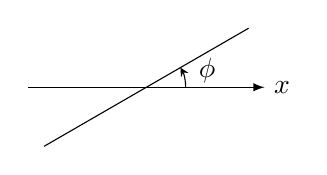
\begin{tikzpicture}
\draw[-latex](-1.5,0)--(1.5,0)node[right]{$x$};
\draw(0,0)++(30:-1.5)--++(30:3);
\draw[-stealth]([shift={(0:0.5)}]0,0) arc (0:30:0.5);
\draw(15:0.8)node[]{$\phi$};
\end{tikzpicture}
\end{subfigure}%
\begin{subfigure}{0.5\textwidth}
\centering
\begin{tikzpicture}
\draw[-latex](-1.5,0)--(1.5,0)node[right]{$x$};
\draw(0,0)++(-45:-1.5)--++(-45:3);
\draw[-stealth]([shift={(0:0.5)}]0,0) arc (0:135:0.5);
\draw(62:0.8)node[]{$\phi$};
\end{tikzpicture}
\end{subfigure}%
\caption{زاویہ میلان $\,x\,$ محور سے گھڑی کی الٹ رخ ناپا جاتا ہے}
\label{شکل_ابتدا_زاویہ_میلان}
\end{figure}

خط کی ڈھلوان \عددی{m} اور زاویہ میلان \عددی{\phi} کا تعلق درج ذیل ہے (شکل \حوالہ{شکل_ابتدا_زاویہ_میلان_اور_ڈھلوان})۔
\begin{align*}
m=\tan \phi
\end{align*}
%
\begin{figure}
\centering
\begin{minipage}{0.45\textwidth}
\centering
\begin{tikzpicture}
\draw[-latex,name path=kX](-0.5,0)--(3.5,0)node[right]{$x$};
\draw[-latex](0,-0.5)--(0,2.25)node[above]{$y$};
\draw[name path=kC](-0.5,-0.5)--++(25:4)node[right]{$L$};
\draw[name intersections={of={kX and kC}}](intersection-1)node[below]{$N_1$};
\draw[thick,-latex](intersection-1)--++(2,0)node[pos=0.5,below]{$\Delta x$}coordinate(kA);
\draw[-stealth]([shift={(0:0.8)}]intersection-1) arc (0:25:0.8);
\draw(intersection-1)++(12:1)node[]{$\phi$};
\path[name path=kY](kA)--++(0,2);
\draw[-latex,thick,name intersections={of={kY and kC}}](kA)--(intersection-1)node[pos=0.5,right]{$\Delta y$};
\draw(1.5,1.5)node[]{$m=\frac{\Delta y}{\Delta x}=\tan \phi$};
\end{tikzpicture}
\caption{غیر انتصابی خط کی ڈھلوان اس کے زاویہ میلان کا ٹینجنٹ ہوتا ہے}
\label{شکل_ابتدا_زاویہ_میلان_اور_ڈھلوان}
\end{minipage}\hfill 
\begin{minipage}{0.45\textwidth}
\centering
\begin{tikzpicture}
\pgfmathsetmacro{\ang}{35}
\draw[-latex,name path=kX](-0.5,0)--(4.75,0)node[right]{$x$};
\draw[-latex](0,-0.25)--++(0,2.5)node[above]{$y$};
\draw(0.5,0)coordinate(kA)node[below]{$A$}++(\ang:-0.5)--++(\ang:4)coordinate[pos=0.8](kC)node[right]{$L_1$ \RL{(ڈھلوان $\,m_1$)}};
\draw[-stealth] ([shift={(0:0.5)}]kA) arc (0:\ang:0.5);
\draw(kA)++(\ang/2:0.8)node[]{$\phi_1$};
\draw[name path=kLB](kC)node[above,yshift={1mm}]{$C$}++(90+\ang:0.75)node[left]{\RL{(ڈھلوان $\,m_2$)}$L_2$}coordinate(kLBS)--++(\ang-90:3.5);
\draw[-stealth,name intersections={of={kX and kLB}}] ([shift={(0:0.5)}]intersection-1) arc (0:90+\ang:0.5);
\draw(intersection-1)coordinate(kB)node[below,xshift={-1mm}]{$B$}++(45+\ang/2:0.8)node[]{$\phi_2$};
\draw[dashed] (kC)--($(0,0)!(kC)!(4,0)$)coordinate(kD)node[below]{$D$}node[pos=0.5,left]{$h$};
\draw([shift={(-90:0.5)}]kC) arc (-90:\ang-90:0.5);
\draw(kC)++(-90+\ang/2:0.8)node[]{$\phi_1$};
\RightAngle{(kLBS)}{(kC)}{(kA)};
\RightAngle{(kC)}{(kD)}{(0,0)};
\draw($(kD)!0.5!(kB)$)node[below]{$a$};
\end{tikzpicture}
\caption{قائمہ خطوط کی ڈھلوان کا تعلق}
\label{شکل_ابتدا_قائمہ_خطوط_ڈھلوان}
\end{minipage}%
\end{figure}

\جزوحصہء{متوازی اور قائمہ خطوط}
متوازی خطوط کا زاویہ میلان ایک جیسا ہو گا لہٰذا  ان  کی ڈھلوان بھی ایک جیسی ہو گی۔اسی طرح ایک جیسی ڈھلوان والے خطوط کا زاویہ میلان ایک جیسا ہو گا لہٰذا یہ متوازی ہوں گے۔

اگر غیر انتصابی خطوط \عددی{L_1} اور \عددی{L_2} آپس میں قائمہ ہوں تب ان کی ڈھلوان \عددی{m_1} اور \عددی{m_2} مساوات \عددی{m_1m_2=-1} کو مطمئن کریں گی۔یوں ایک خط کی ڈھلوان کا منفی معکوس  دوسرے خط کی ڈھلوان کے برابر ہو گا، یعنی:
\begin{align*}
m_1=-\frac{1}{m_2},\quad m_2=-\frac{1}{m_1}
\end{align*}
شکل \حوالہ{شکل_ابتدا_قائمہ_خطوط_ڈھلوان} میں قائمہ خطوط دکھائے گئے ہیں جہاں  \عددی{m_1=\tan\phi_1=\tfrac{a}{h}}  اور \عددی{m_2=\tan\phi_2=-\tfrac{h}{a}} ہیں۔یوں \عددی{m_1m_2=(\tfrac{a}{h})(-\tfrac{h}{a})=-1} ہو گا۔

\جزوحصہء{خطوط کے مساوات}
سیدھے خطوط کی مساوات نسبتاً سادہ ہوتی ہیں۔\عددی{x} محور کے نقطہ \عددی{a} سے گزرتے انتصابی خط پر ہر نقطے کی \عددی{x} محدد \عددی{a} ہو گی۔یوں اس انتصابی خط کی مساوات \عددی{x=a} ہو گی۔اسی طرح \عددی{y} محور کے نقطہ \عددی{b} سے گزرتے افقی خط کی مساوات \عددی{y=b} ہو گی۔

\ابتدا{مثال}\شناخت{مثال_ابتدا_افقی_انتصابی_مساوات}
نقطہ \عددی{(4,2)} سے گزرتے افقی اور انتصابی خطوط کے مساوات بالترتیب \عددی{y=2} اور \عددی{x=4} ہوں گی (شکل \حوالہ{شکل_مثال_ابتدا_افقی_انتصابی_مساوات})۔
\begin{figure}
\centering
\begin{tikzpicture}
\draw[-latex](-0.5,0)--(5.5,0)node[right]{$x$};
\draw[-latex](0,-0.25)--(0,3)node[above]{$y$};
\foreach \x in {1,2,3,4,5}{\draw(\x,0)node[below]{$\x$}--++(0,0.1);}
\foreach \y in {1,2}{\draw(0,\y)node[left]{$\y$}--++(0.1,0);}
\draw(-0.5,2)--(5.5,2)node[right]{$y=2$};
\draw(4,-0.25)--(4,3)node[right]{$x=4$};
\draw(4,2)node[circ]{}node[below right]{$(4,2)$};
\draw(0,0)node[below left]{$0$};
\end{tikzpicture}
\caption{افقی اور انتصابی خطوط کی مساوات (مثال \حوالہ{مثال_ابتدا_افقی_انتصابی_مساوات})}
\label{شکل_مثال_ابتدا_افقی_انتصابی_مساوات}
\end{figure}
\انتہا{مثال}
%==========================

اگر ہمیں غیر انتصابی سیدھے خط \عددی{L} کی ڈھلوان معلوم ہو اور اس خط پر کوئی نقطہ \عددی{N_1(x_1,y_1)} معلوم ہو تب ہم اس کی مساوات لکھ سکتے ہیں۔اگر اس خط پر \عددی{N(x,y)} کوئی دوسرا نقطہ ہو تب
\begin{align*}
m=\frac{y-y_1}{x-x_1}
\end{align*}
ہو گا جس کو

\begin{align*}
y-y_1=m(x-x_1)\quad \implies \quad y=y_1+m(x-x_1)
\end{align*}
لکھا جا سکتا ہے جو اس خط کی مساوات ہے۔

\ابتدا{تعریف}
نقطہ \عددی{(x_1,y_1)} سے گزرتے ایسا خط جس کی ڈھلوان \عددی{m} ہو کی مساوات \عددی{y=y_1+m(x-x_1)} ہو گی جس کو  خط کی \اصطلاح{نقطہ-ڈھلوان مساوات}\فرہنگ{مساوات!نقطہ-ڈھلوان}\حاشیہب{point-slope equation}\فرہنگ{equation!point-slope} ہے۔
\انتہا{تعریف}
%=======================

\ابتدا{مثال}
نقطہ \عددی{(3,2)} سے گزرتا خط جس کی ڈھلوان \عددی{-\tfrac{2}{3}}  ہو کی مساوات تلاش کریں۔\\
حل:\quad
\begin{align*}
y=2-\frac{2}{3}(x-3)\quad \implies \quad y=-\frac{2}{3}x+4
\end{align*}
\انتہا{مثال}
%======================
\ابتدا{مثال}\شناخت{مثال_ابتدا_مساوات_خط_دو_نقطے}
نقطہ \عددی{(-2,-1)} اور \عددی{(3,4)} سے گزرتا خط کی مساوات تلاش کریں۔\\
حل:\quad
اس خط کی ڈھلوان
\begin{align*}
m=\frac{-1-4}{-2-3}=\frac{-5}{-5}=1
\end{align*}
ہے۔ہم دونوں نقطوں میں سے کوئی ایک لیتے ہوئے خط کی مساوات حاصل کر سکتے ہیں۔طریقہ کار درج ذیل ہے۔
\begin{gather*}
\begin{aligned}
&\text{\RL{نقطہ $(x_1,y_1)=(-2,-1)$ لیتے ہیں}}\\[0.5em]
&y=-1+1\cdot(x-x(-2))\\
&y=-1+x+2\\
&y=x+1
\end{aligned}\quad\quad
\begin{aligned}
&\text{\RL{نقطہ $(x_1,y_1)=(3,4)$ لیتے ہیں}}\\[0.5em]
&y=4+1\cdot(x-3)\\
&y=4+x-3\\
&y=x+1
\end{aligned}
\end{gather*}
آپ نے دیکھا کہ دونوں سے ایک جیسی مساوات حاصل ہوتی ہے (شکل \حوالہ{شکل_مثال_ابتدا_مساوات_خط_دو_نقطے})۔
\begin{figure}
\centering
\begin{minipage}{0.45\textwidth}
\centering
\begin{tikzpicture}[x={0.75cm},y={0.75cm}]
\draw[-latex](-3,0)--(4,0)node[right]{$x$};
\draw[-latex](0,-1.5)--(0,5)node[above]{$y$};
\foreach \x in {-2,-1,1,2,3}{\draw(\x,0)--++(0,0.1);}
\foreach \y in {-1,1,2,3,4}{\draw(0,\y)--++(0.1,0);}
\draw(-2,0)node[below,xshift={-1mm}]{$-2$};
\draw(3,0)node[below]{$3$};
\draw(0,-1)node[left]{$-1$};
\draw(0,4)node[left]{$4$};
\draw[shorten >=-0.5cm, shorten <=-0.5cm](-2,-1)node[circ]{}node[yshift={-5mm}]{$(-2,-1)$}--(3,4)node[circ]{}node[below right]{$(3,4)$}node[pos=0.7,below right]{$y=x+1$};
\end{tikzpicture}
\caption{دو نقطوں میں گزرتے خط کی مساوات (مثال \حوالہ{مثال_ابتدا_مساوات_خط_دو_نقطے})}
\label{شکل_مثال_ابتدا_مساوات_خط_دو_نقطے}
\end{minipage}\hfill
\begin{minipage}{0.45\textwidth}
\centering
\begin{tikzpicture}
\draw[-latex,name path=kX](-0.5,0)--(4,0)node[right]{$x$};
\draw[-latex,name path=kY](0,-0.25)--(0,4)node[above]{$y$};
\draw(0,0)node[below left]{$0$};
\draw[name path=kC](-0.5,3.5)--(3.5,-0.25);
\draw[name intersections={of={kC and kX}}] (intersection-1)node[below]{$a$}--++(0,0.1);
\draw[name intersections={of={kC and kY}}] (intersection-1)node[left]{$b$}--++(0.1,0);
\end{tikzpicture}
\caption{غیر انتصابی اور غیر افقی خط کے محوری قطعات}
\label{شکل_ابتدا_قطع_محور}
\end{minipage}%
\end{figure}
\انتہا{مثال}
%====================
غیر انتصابی خط \عددی{y}  محور کو جس نقطہ پر قطع کرتا ہو اس نقطہ کو خط کا \اصطلاح{\عددی{y} قطع}\فرہنگ{قطع!وائے}\حاشیہب{y-intercept}\فرہنگ{intercept!y} کہتے ہیں۔اسی طرح غیر افقی خط جس نقطہ پر \عددی{x} محور کو قطع کرتا ہو اس نقطہ کو خط کا \اصطلاح{\عددی{x} قطع}\فرہنگ{قطع!ایکس}\حاشیہب{x-intercept}\فرہنگ{intercept!x} کہتے ہیں (شکل \حوالہ{شکل_ابتدا_قطع_محور})۔

غیر انتصابی خط جو \عددی{y} محور کو \عددی{(0,b)} پر قطع کرتا ہو کی مساوات 
\begin{align*}
y=b+m(x-0)\quad \implies \quad y=mx+b
\end{align*}
ہو گی۔

\ابتدا{تعریف}
درج ذیل مساوات 
\begin{align*}
y=b+m(x-0)\quad \implies \quad y=mx+b
\end{align*}
کو خط  کی \اصطلاح{ڈھلوان-قطع مساوات}\فرہنگ{مساوات!ڈھلوان-قطع}\حاشیہب{slope-intercept equation}\فرہنگ{equation!slope-intercept} کہتے ہیں۔اس خط کی ڈھلوان \عددی{m} ہے اور یہ \عددی{y} محور کو \عددی{b} پر قطع کرتا ہے۔
\انتہا{تعریف}

%======================
\ابتدا{مثال}
خط \عددی{y=3x-7} کی ڈھلوان \عددی{m=3} ہے جبکہ یہ \عددی{y} محور کو \عددی{-7} پر قطع کرتا ہے۔
\انتہا{مثال}
%========================

درج ذیل مساوات کو \اصطلاح{عمومی خطی مساوات}\فرہنگ{مساوات!عمومی خطی}\حاشیہب{general linear equation}\فرہنگ{equation!general linear} کہتے ہیں۔
\begin{align*}
Ax+By=C\quad\quad\quad (\text{\RL{$A\,$ اور $\,B\,$ دونوں ایک ساتھ صفر نہیں ہیں}})
\end{align*}
ہر سیدھا خط (بشمول غیر معین ڈھلوان کا خط) کو عمومی خطی مساوات کی صورت میں لکھا جا سکتا ہے۔ 

\ابتدا{مثال}
خط \عددی{8x+5y=20} کی \عددی{y} قطع تلاش کریں۔\\
حل:\quad
ہم مساوات کو ڈھلوان-قطع روپ میں لکھ کر \عددی{y} قطع کو مساوات سے حاصل کرتے ہیں۔
\begin{align*}
8x+5y&=20\\
5y&=-8x+20\\
y&=-\frac{8}{5}x+4
\end{align*}
یوں خط کی ڈھلوان \عددی{-\tfrac{8}{5}} اور \عددی{y} قطع \عددی{4} ہے۔
\انتہا{مثال}
%======================

\ابتدا{مثال}
مبدا سے گزرتے خطوط کی مساواتیں۔\\
چونکہ ان خطوط کا \عددی{y} قطع \عددی{0} ہو گا لہٰذا ان کی مساوات \عددی{y=mx} ہو گی۔ شکل \حوالہ{شکل_ابتدا_مبدا_گزرتا_خط} میں چند مثالیں دکھائی گئی ہیں۔
\begin{figure}
\centering
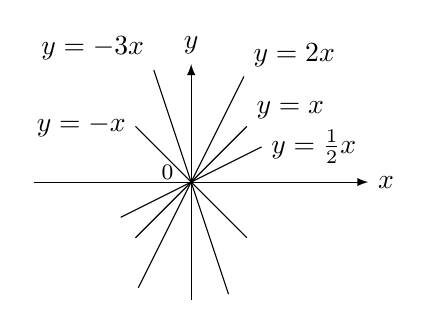
\begin{tikzpicture}
\pgfmathsetmacro{\angA}{atan(1)}
\pgfmathsetmacro{\angB}{atan(2)}
\pgfmathsetmacro{\angC}{atan(3)}
\pgfmathsetmacro{\angD}{atan(1/2)}
\draw[-latex](-2,0)--(2.25,0)node[right]{$x$};
\draw[-latex](0,-1.5)--(0,1.5)node[above]{$y$};
\draw(0,0)++(\angA:-1)--++(\angA:2)node[right,yshift={2mm}]{$y=x$};
\draw(0,0)++(180-\angA:-1)--++(180-\angA:2)node[left]{$y=-x$};
\draw(0,0)++(\angB:-1.5)--++(\angB:3)node[above right]{$y=2x$};
\draw(0,0)++(180-\angC:-1.5)--++(180-\angC:3)node[above left]{$y=-3x$};
\draw(0,0)++(\angD:-1)--++(\angD:2)node[right]{$y=\frac{1}{2}x$};
\draw(-0.3,0)node[yshift={1.2mm},font=\footnotesize]{$0$};
\end{tikzpicture}
\caption{مبدا سے گزرتا خط کی مساوات $\,y=mx\,$ ہے جہاں $\,m\,$ خط کی ڈھلوان ہے}
\label{شکل_ابتدا_مبدا_گزرتا_خط}
\end{figure}
\انتہا{مثال}
%========================

\جزوحصہء{خطوط اور خط کی اہمیت}
شعاع سیدھے خط پر چلتی ہے۔اسی طرح ساکن جسم کشش ثقل کی بنا سیدھے خط پر حرکت کرتا ہے۔ہم عموماً خط کی مساوات (جنہیں \اصطلاح{خطی مساوات}\فرہنگ{خطی!مساوات}\حاشیہب{linear equations}\فرہنگ{linear!equations} کہتے ہیں) استعمال کرتے ہوئے اس طرح کی طبعی اعمال پر غور کرتے ہیں۔ 

بہت سارے اہم مقدار آپس میں خطی تعلق رکھتے ہیں۔یہ جانتے ہوئے کہ دو مقدار آپس میں خطی تعلق رکھتے ہیں، ہم ان کی مطابقتی قیمتوں کی کسی بھی دو جوڑیوں سے یہ تعلق دریافت کر سکتے ہیں۔ڈھلوان سے ہمیں چڑھائی معلوم ہوتی ہے یا مقداروں کی تبدیلی کی شرح معلوم ہوتی ہے۔اسی بنا احصاء میں ڈھلوان کلیدی کردار ادا کرتا ہے۔ 

\ابتدا{مثال}
برقی دور میں برقی دباو \عددی{V} اور برقی رو \عددی{I} کا تعلق \عددی{V=IR} ہے جو خطی مساوات ہے۔اس مساوات کی ڈھلوان \عددی{R} ہے جس کو مزاحمت کہتے ہیں۔
\انتہا{مثال}

\جزوحصہء{سوالات}
\موٹا{بڑھوتری اور کٹوتی}\\
سوال \حوالہ{سوال_ابتدا_بڑھوتری_کٹوتی_الف} تا سوال \حوالہ{سوال_ابتدا_بڑھوتری_کٹوتی_ب} میں ایک ذرہ \عددی{A} سے \عددی{B} منتقل ہوتا ہے۔اس کی بڑھوتری \عددی{\Delta x} اور \عددی{\Delta y} تلاش کریں اور \عددی{A} سے \عددی{B} تک فاصلہ تلاش کریں۔

\ابتدا{سوال}\شناخت{سوال_ابتدا_بڑھوتری_کٹوتی_الف}
$A(-3,2),\, B(-1,-2)$\\
جواب:\quad
$2,-4;2\sqrt{5}$
\انتہا{سوال}
%========================
\ابتدا{سوال}
$A(-1,-2),\, B(-3,2)$
\انتہا{سوال}
%================================
\ابتدا{سوال}
$A(-3.2,-2),\, B(-8.1,-2)$\\
جواب:\quad
$-4.9,0;4.9$
\انتہا{سوال}
%================================
\ابتدا{سوال}\شناخت{سوال_ابتدا_بڑھوتری_کٹوتی_ب}
$A(\sqrt{2},4),\, B(0,1.5)$
\انتہا{سوال}
%========================
سوال \حوالہ{سوال_ابتدا_ترسیم_کریں_الف} تا سوال \حوالہ{سوال_ابتدا_ترسیم_کریں_ب} میں دیا گیا مساوات ترسیم کریں۔ترسیم پر تبصرہ کریں۔

%======================
\ابتدا{سوال}\شناخت{سوال_ابتدا_ترسیم_کریں_الف}
$x^2+y^2=1$\\
جواب:\quad
اکائی دائرہ
\انتہا{سوال}
%======================
\ابتدا{سوال}
$x^2+y^2=2$
\انتہا{سوال}
%======================
\ابتدا{سوال}
$x^2+y^2\le 3$\\
جواب:\quad
رداس \عددی{\sqrt{3}} کا دائرہ اور اس کی اندرون۔دائرے کا مرکز مبدا پر ہے۔
\انتہا{سوال}
%======================
\ابتدا{سوال}\شناخت{سوال_ابتدا_ترسیم_کریں_ب}
$x^2+y^2=0$
\انتہا{سوال}
%======================
\موٹا{ڈھلوان، خطوط اور محوری قطعات}\\
سوال \حوالہ{سوال_ابتدا_ڈھلوان_الف} تا سوال \حوالہ{سوال_ابتدا_ڈھلوان_ب} دیے گئے نقطوں کو ترسیم کریں۔ جہاں ممکن ہو، نقطوں کو ملانے والے خط کی  ڈھلوان تلاش کریں۔ خط \عددی{AB} کی قائمہ خطوط کی ڈھلوان تلاش کریں۔\\

\ابتدا{سوال}\شناخت{سوال_ابتدا_ڈھلوان_الف}
$A(-1,2),\,B(-2,-1)$\\
جواب:\quad
$m_{\perp}=-\tfrac{1}{3}$
\انتہا{سوال}
%========================
\ابتدا{سوال}
$A(-2,1),\,B(2,-2)$
\انتہا{سوال}
%========================
\ابتدا{سوال}
$A(2,3),\,B(-1,3)$\\
جواب:\quad
\عددی{m_{\perp}} غیر معین ہے۔
\انتہا{سوال}
%========================
\ابتدا{سوال}\شناخت{سوال_ابتدا_ڈھلوان_ب}
$A(-2,0),\,B(-2,-2)$
\انتہا{سوال}
%========================

سوال \حوالہ{سوال_ابتدا_انتصابی_الف} تا سوال \حوالہ{سوال_ابتدا_انتصابی_ب} میں دیے گئے نقطہ سے گزرتا (الف) انتصابی خط اور (ب) افقی خط کی مساوات تلاش کریں۔\\

\ابتدا{سوال}\شناخت{سوال_ابتدا_انتصابی_الف}
$(-1,\tfrac{4}{3})$\\
جواب:\quad
(الف) 
$x=-1$\quad 
(ب) 
$y=\tfrac{4}{3}$
\انتہا{سوال}
%============================
\ابتدا{سوال}
$(\sqrt{2},-1.3)$
\انتہا{سوال}
%============================
\ابتدا{سوال}
$(0,-\sqrt{2})$\\
جواب:\quad
(الف) \عددی{x=0} 
\quad
$y=-\sqrt{2}$
\انتہا{سوال}
%============================
\ابتدا{سوال}\شناخت{سوال_ابتدا_انتصابی_ب}
$(-\pi,0)$
\انتہا{سوال}
%============================
سوال \حوالہ{سوال_ابتدا_مساوات_تلاش_الف} تا سوال \حوالہ{سوال_ابتدا_مساوات_تلاش_ب} میں خط کی مساوات تلاش کریں۔خط کی تفصیل دی گئی ہے۔

\ابتدا{سوال}\شناخت{سوال_ابتدا_مساوات_تلاش_الف}
نقطہ \عددی{(-1,1)} سے گزرتا خط جس کی ڈھلوان \عددی{-1} ہو۔\\
جواب:\quad
$y=-x$
\انتہا{سوال}
%========================
\ابتدا{سوال}
نقطہ \عددی{(2,-3)} سے گزرتا خط جس کی ڈھلوان \عددی{\tfrac{1}{2}} ہو۔
\انتہا{سوال}
%========================
\ابتدا{سوال}
نقطہ \عددی{(3,4)} اور \عددی{(-2,5)} سے گزرتا خط۔\\
جواب:\quad
$y=-\tfrac{x}{5}+\tfrac{23}{5}$
\انتہا{سوال}
%========================
\ابتدا{سوال}
نقطہ \عددی{(-8,0)} اور \عددی{(-1,3)} سے گزرتا خط۔
\انتہا{سوال}
%========================
\ابتدا{سوال}
ڈھلوان \عددی{-\tfrac{5}{4}} اور \عددی{y} قطع \عددی{6} ہے۔\\
جواب:\quad
$y=-\tfrac{5}{4}x+6$
\انتہا{سوال}
%========================
\ابتدا{سوال}
ڈھلوان \عددی{\tfrac{1}{2}} اور \عددی{y} قطع \عددی{-3} ہے۔
\انتہا{سوال}
%========================
\ابتدا{سوال}
نقطہ \عددی{(-12,-9)} سے گزرتا جس کی ڈھلوان \عددی{0} ہو۔\\
جواب:\quad
$y=-9$
\انتہا{سوال}
%========================
\ابتدا{سوال}
نقطہ \عددی{(\tfrac{1}{3},2)} سے گزرتا جس کی کوئی  ڈھلوان نہ ہو۔
\انتہا{سوال}
%========================
\ابتدا{سوال}
جس کا \عددی{x} قطع \عددی{-1} اور \عددی{y} قطع \عددی{4} ہو۔\\
جواب:\quad
$y=4x+4$
\انتہا{سوال}
%=====================
\ابتدا{سوال}
جس کا \عددی{x} قطع \عددی{2} اور \عددی{y} قطع \عددی{-6} ہو۔
\انتہا{سوال}
%=====================
\ابتدا{سوال}
جو نقطہ \عددی{(5,-1)} سے گزرتا ہو اور خط \عددی{2x+5y=15} کے متوازی ہو۔\\
جواب:\quad
$y=-\tfrac{2}{5}x+1$
\انتہا{سوال}
%====================
\ابتدا{سوال}
جو نقطہ \عددی{(-\sqrt{2},\sqrt{2})} سے گزرتا ہو اور خط \عددی{\sqrt{2}x+5y=\sqrt{3}} کے متوازی ہو۔
\انتہا{سوال}
%====================
\ابتدا{سوال}
نقطہ \عددی{4,10} سے گزرتا اور خط \عددی{6x-3y=13} کا قائمہ ہو۔\\
جواب:\quad
$y=-\tfrac{x}{2}+12$
\انتہا{سوال}
%=====================
\ابتدا{سوال}\شناخت{سوال_ابتدا_مساوات_تلاش_ب}
نقطہ \عددی{(0,1)} سے گزرتا اور خط \عددی{8x-13y=13} کا قائمہ۔

\انتہا{سوال}
%====================
خط کا \عددی{x} قطع اور \عددی{y} قطع تلاش کریں۔ان معلومات کو استعمال کرتے ہوئے خط ترسیم کریں۔ (سوال \حوالہ{سوال_ابتدا_محوری_مقطع_الف} تا سوال \حوالہ{سوال_ابتدا_محوری_مقطع_ب})

\ابتدا{سوال}\شناخت{سوال_ابتدا_محوری_مقطع_الف}
$3x+4y=12$\\
جواب:\quad
قطع \عددی{4=x}،
\quad 
قطع \عددی{3=y} 

\انتہا{سوال}
%=======================
\ابتدا{سوال}
$x+2y=-4$
\انتہا{سوال}
%=======================
\ابتدا{سوال}
$\sqrt{2}x-\sqrt{3}y=\sqrt{6}$\\
جواب:\quad
قطع \عددی{\sqrt{3}=x}،
\quad
قطع \عددی{-\sqrt{2}=y}
\انتہا{سوال}
%=======================
\ابتدا{سوال}\شناخت{سوال_ابتدا_محوری_مقطع_ب}
$1.5x-y=-3$
\انتہا{سوال}
%=======================
\ابتدا{سوال}
کیا \عددی{Ax+By=C_1} اور \عددی{Bx-Ay=C_2} (جہاں \عددی{A\ne 0} اور \عددی{B\ne 0} ہیں) میں کوئی خاص تعلق پایا جاتا ہے۔تعلق کی وجہ بیان کریں۔\\
جواب:\quad
جی ہاں۔خطوط قائمہ ہیں چونکہ ان کی ڈھلوان \عددی{-\tfrac{A}{B}} اور \عددی{\tfrac{B}{A}} ایک دوسرے کے منفی معکوس ہیں۔
\انتہا{سوال}
%=======================
\ابتدا{سوال}
کیا \عددی{Ax+By=C_1} اور \عددی{Ax+By=C_2} (جہاں \عددی{A\ne 0} اور \عددی{B\ne 0} ہیں) میں کوئی خاص تعلق پایا جاتا ہے۔تعلق کی وجہ بیان کریں۔
\انتہا{سوال}
%==========================
\موٹا{بڑھوتری اور حرکت}

\ابتدا{سوال}
ایک ذرہ کا ابتدائی مقام \عددی{A(-2,3)} ہے جبکہ اس کی بڑھوتری \عددی{\Delta x=5}، \عددی{\Delta y=-6} ہیں۔ذرہ کا اختتامی مقام تلاش کریں۔\\
جواب:\quad
$(3,-3)$
\انتہا{سوال}
%=====================
\ابتدا{سوال}
ایک ذرہ کا ابتدائی مقام \عددی{A(6,0)} ہے جبکہ اس کی بڑھوتری \عددی{\Delta x=-6}، \عددی{\Delta y=0} ہیں۔ذرہ کا اختتامی مقام تلاش کریں۔
\انتہا{سوال}
%=====================
\ابتدا{سوال}
ایک ذرہ \عددی{A(x,y)} سے \عددی{B(3,-3)} منتقل ہوتا ہے۔اس کی بڑھوتری \عددی{\Delta x=5} اور \عددی{\Delta y=6} ہیں۔ابتدائی نقطہ تلاش کریں۔\\
جواب:\quad
$(-2,-9)$
\انتہا{سوال}
%=======================
\ابتدا{سوال}
ایک ذرہ \عددی{A(1,0)} سے حرکت کرتے ہوئے مبدا کے گرد گھڑی کی الٹ رخ ایک چکر مکمل کرنے کے بعد \عددی{A(1,0)} کو واپس لوٹتا ہے۔اس کے محدد میں کل تبدیلی کیا ہے؟
\انتہا{سوال}
%====================
\موٹا{عملی استعمال}\\

\ابتدا{سوال}\ترچھا{پانی میں دباو}\quad 
پانی میں \عددی{d} گہرائی پر غوطہ خور \عددی{p} دباو محسوس کرے گا جہاں \عددی{p=kd+1} ہے جہاں \عددی{k} مستقل ہے۔پانی کی سطح پر یہ \عددی{1} کرہ ہوائی دباو پایا جاتا ہے۔ \عددی{100} میٹر گہرائی پر تقریباً  \عددی{10.94} کرہ ہوائی دباو پایا جاتا ہے۔\عددی{50} میٹر گہرائی پر دباو کیا ہو گا؟\\
جواب:\quad
\عددی{5.97} کرہ ہوائی دباو
\انتہا{سوال}
%=====================
\ابتدا{سوال}\ترچھا{انعکاس شعاع}\quad
ربع دوم سے خط \عددی{x+y=1} پر آمدی شعاع \عددی{x} محور سے منعکس ہوتی ہے۔زاویہ آمد اور زاویہ انعکاس برابر ہوتے ہیں۔انعکاسی شعاع کس خط پر حرکت کرے گی؟
\انتہا{سوال}
%======================
\ابتدا{سوال}\موٹا{سیلسیئس بالمقابل فارن ہائیٹ}\quad 
سیلسیئس بالمقابل فارن ہائیٹ مستوی \عددی{FC} میں \عددی{C=\tfrac{5}{9}(F-32)} ترسیم کریں جو فارن ہائیٹ سے سیلسیئس حاصل کرنے کا کلیہ ہے۔اسی جگہ \عددی{F=C} ترسیم کریں۔کیا کوئی ایسی درجہ حرارت پائی جاتی ہے جس پر دونوں پیمانے ایک جیسی اعدادی جواب دیں؟\\
جواب:\quad
جی ہاں۔ \عددی{C=F=-40^{\circ}}
\انتہا{سوال}
%=====================

\موٹا{نظریہ اور مثالیں}\\

\ابتدا{سوال}
ایک مثلث کے راس \عددی{A(1,2)}، \عددی{B(5,5)} اور \عددی{C(4,-2)} پر پائے جاتے ہیں۔مثلث کے تینوں اضلاع کی لمبائیاں تلاش کرتے ہوئے ثابت کریں کہ یہ مساوی الساقین مثلث ہے اور متساوی الاضلاع مثلث نہیں ہے۔  
\انتہا{سوال}
%======================
\ابتدا{سوال}
ایک مثلث کے راس \عددی{A(0,0)}، \عددی{B(1,\sqrt{3})} اور \عددی{C(2,0)} ہیں۔دکھائیں کہ یہ متساوی الاضلاع مثلث ہے۔
\انتہا{سوال}
%===================
\ابتدا{سوال}
دکھائیں کہ \عددی{A(2,-1)}، \عددی{B(1,3)} اور \عددی{C(-3,2)} چوکور کی راسیں ہیں۔چوتھی راس تلاش کریں۔ 
\انتہا{سوال}
%=================
\ابتدا{سوال}
تین مختلف متوازی الاضلاع کے راس \عددی{(-1,1)}، \عددی{(2,0)} اور \عددی{(2,3)} ہیں۔تینوں کی چوتھی راس تلاش کریں۔\\
جواب:\quad
$(-1,4), (-1,-2), (5,2)$
\انتہا{سوال}
%=================
\ابتدا{سوال}\شناخت{سوال_ابتدا_گھومنا}
مبدا کے گرد گھڑی مخالف \عددی{90^{\circ}} گھمانے سے نقطہ \عددی{(2,0)} اور \عددی{(0,3)} بالترتیب \عددی{(0,2)} اور \عددی{(-3,0)} منتقل ہوتے ہیں (شکل \حوالہ{شکل_سوال_ابتدا_گھومنا})۔درج ذیل نقطے کہاں منتقل ہوں گے؟
\begin{multicols}{3}
\begin{enumerate}[a)]
\item 
$(4,1)$
\item
$(-2,-3)$
\item
$(2,-5)$
\item
$(x,0)$
\item
$(0,y)$
\item
$(x,y)$
\item
کونسا نقطہ \عددی{(10,3)} پر منتقل ہو گا؟
\end{enumerate}
\end{multicols}
%
\begin{figure}
\centering
\begin{tikzpicture}[x=0.5cm,y=0.5cm]
\draw[-latex](-4,0)--(6,0)node[right]{$x$};
\draw[-latex](0,-4)--(0,3.5)node[above]{$y$};
\draw(2,0)node[circ]{}node[below]{$(2,0)$};
\draw[-stealth]([shift={(0:2)}]0,0) arc (0:90:2)node[circ]{}node[left]{$(0,2)$};
\draw(0,3)node[circ]{}node[right]{$(0,3)$};
\draw[-stealth]([shift={(90:3)}]0,0) arc (90:180:3)node[circ]{}node[below]{$(-3,0)$};
\draw(-2,-3)node[left]{$(-2,-3)$}node[circ]{};
\draw[-stealth]([shift={(236.31:3.60555)}]0,0) arc (236.31:326.31:3.60555)node[circ]{};
\draw(4,1)node[circ]{}node[above]{$(4,1)$};
\end{tikzpicture}
\caption{گھڑی مخالف $90^{\circ}$ گھومنا (سوال \حوالہ{سوال_ابتدا_گھومنا})}
\label{شکل_سوال_ابتدا_گھومنا}
\end{figure}
\انتہا{سوال}
%======================
\ابتدا{سوال}
\عددی{k} کی کس قیمت کے لئے خط \عددی{2x+ky=3} اور خط \عددی{4x+y=1} قائمہ ہوں گے۔ \عددی{k}کی کس قیمت کے لئے یہ خطوط متوازی ہوں گے؟\\
جواب:\quad
$k=-8,\quad k=\tfrac{1}{2}$
\انتہا{سوال}
%===================
\ابتدا{سوال}
وہ خط تلاش کریں جو نقطہ \عددی{(1,2)} اور خط \عددی{x+2y=3} اور \عددی{2x-3y=-1} کے انقطاعی نقطہ سے گزرتا ہو۔
\انتہا{سوال}
%===================
\ابتدا{سوال}
دکھائیں کہ \عددی{A(x_1,y_1)} اور \عددی{B(x_2,y_2)} کو ملانے والے قطع کا وسط \عددی{(\tfrac{x_1+x_2}{2},\tfrac{y_1+y_2}{2})} ہو گا۔
\انتہا{سوال}
%========================
\ابتدا{سوال}\ترچھا{نقطہ سے خط تک فاصلہ}\quad
نقطہ \عددی{N(x_0,y_0)} سے خط \عددی{L:Ax+By=C} تک فاصل درج ذیل قدم لیتے ہوئے حاصل کیا جا سکتا ہے۔
\begin{itemize}
\item
\عددی{L} کی قائمہ اور \عددی{N} سے گزرتے خط \عددی{Q} کی مساوات تلاش کریں۔
\item
خط \عددی{Q} اور \عددی{L} کا نقطہ تقاطع \عددی{M} تلاش کریں۔
\item
\عددی{N} سے \عددی{M} تک فاصلہ تلاش کریں۔
\end{itemize}
اس طریقہ کو استعمال کرتے ہوئے درج ذیل نقطوں کا دیے گئے خط سے فاصل تلاش کریں۔
\begin{multicols}{2}
\begin{enumerate}[a)]
\item
$N(2,1), L:y=x+2$
\item
$N(4,6), L:4x+3y=12$
\item
$N(a,b),L:x=-1$
\item
$N(x_0,y_0), L:Ax+By=C$
\end{enumerate}
\end{multicols}
\انتہا{سوال}
%==================

\حصہ{تفاعل}
حقیقی دنیا کو ریاضیاتی روپ میں تفاعل کے ذریعہ بیان کیا جاتا ہے۔اس حصہ میں تفاعل پر غور کیا جائے گا اور ایسے چند تفاعل پر غور کیا جائے گا جو احصاء میں پائے جائیں گے۔

\جزوحصہء{تفاعل}
سطح سمندر سے بلندی پر پانی ابلنے کا درجہ حرارت منحصر ہے۔زیادہ بلندی پر پانی کم درجہ حرارت پر ابلتا ہے۔اسی طرح سرمایہ کاری پر منافع سرمایہ کاری کے دورانیے پر منحصر ہے۔ان دونوں مثالوں میں ایک متغیر، جس کو ہم \عددی{y} کہہ سکتے ہیں، کا دارومدار دوسرے متغیر، جس کو ہم \عددی{x} کہہ سکتے ہیں، پر منحصر ہے۔چونکہ \عددی{y} کی قیمت مکمل طور پر \عددی{x} تعین کرتا ہے لہٰذا \عددی{y} کو \عددی{x} کا تفاعل کہتے ہیں۔

زیر غور مسئلہ کو دیکھ کر متغیرات منتخب کیے جاتے ہیں۔یوں دائرے کے رقبہ کی بات کرتے ہوئے رقبہ کو \عددی{A} اور رداس کو \عددی{r} سے ظاہر کیا جاتا ہے۔چونکہ \عددی{A=\pi r^2} ہے لہٰذا ہم کہتے ہیں کہ رداس \عددی{r} کا رقبہ \عددی{A} تفاعل ہے۔مساوات \عددی{A=\pi r^2} وہ قاعدہ ہے جس کی مدد سے \عددی{r} کی ہر قیمت  کے لئے \عددی{A} کی \ترچھا{یکتا} قیمت  تلاش کی جا سکتی ہے۔ 

رداس کی تمام ممکنہ قیمتوں کے سلسلہ کو تفاعل کا \اصطلاح{دائرہ کار}\فرہنگ{دائرہ کار}\حاشیہب{domain}\فرہنگ{domain} کہتے ہیں جبکہ تفاعل کی تمام قیمتوں کے سلسلہ کو تفاعل کا \اصطلاح{سعت}\فرہنگ{سعت}\حاشیہب{range}\فرہنگ{range} کہتے ہیں۔چونکہ رداس کی قیمت منفی نہیں ہو سکتی ہے لہٰذا تفاعل کا دائرہ کار اور سعت دونوں وقفہ \عددی{[0,\infty)} پر مشتمل ہوں گے جو تمام غیر منفی حقیقی اعداد کا سلسلہ ہے۔

ریاضیاتی تفاعل کا دائرہ کار اور اس کا سعت چیزوں کا سلسلہ ہو سکتے ہیں؛ ضروری نہیں ہے کہ یہ اعداد ہی ہوں۔اس کتاب میں زیادہ تر دائرہ کار اور سعت اعدادی ہوں گے۔

احصاء میں ہم عموماً کلی تفاعل کی بات کرتے ہیں۔ہمارے ذہن میں کوئی مخصوص تفاعل نہیں ہوتا ہے۔ہم
\begin{align*}
y=f(x)\quad \quad \text{\RL{($y$ برابر ہے $x$ کا $f$)}}
\end{align*}
لکھتے ہوئے کہنا چاہتے ہیں کہ متغیر \عددی{y}، متغیر \عددی{x}  کا تفاعل  ہے۔یہاں \عددی{f} تفاعل کو ظاہر کرتی ہے جبکہ داخلی قیمت \عددی{x} \اصطلاح{غیر تابع متغیر}\فرہنگ{غیر تابع متغیر}\حاشیہب{independent variable}\فرہنگ{independent variable} ہے اور خارجی قیمت \عددی{y} \اصطلاح{تابع متغیر}\فرہنگ{تابع متغیر}\حاشیہب{dependent variable}\فرہنگ{dependent variable} ہیں۔\عددی{x} کی قیمت تفاعل کی دائرہ کار میں سے ہو گی جبکہ \عددی{y} کی قیمت تفاعل کی سعت میں سے ہو گی۔ 

\ابتدا{تعریف}
سلسلہ \عددی{D} سے سلسلہ \عددی{R} تک تفاعل \عددی{f(x)} اس قاعدہ کو کہتے ہیں جو \عددی{D} میں ہر رکن \عددی{x} کو \عددی{R} کا \ترچھا{یکتا} رکن \عددی{f(x)} مختص کرتا ہے۔
\انتہا{تعریف}
%=========================

اس تعریف کے تحت \عددی{D=D(f)} (جس کو $D$ کا $f$ پڑھتے ہیں) تفاعل \عددی{f} کا دائرہ کار ہے اور \عددی{f} کا سعت \عددی{R} کا حصہ ہے (شکل \حوالہ{شکل_ابتدا_تفاعل_دائرہ_کار_اور_سعت})۔
\begin{figure}
\centering
\begin{minipage}{0.45\textwidth}
\centering
\begin{tikzpicture}
\draw[rotate=30] (0,0) circle (1cm and 0.5cm);
\draw(0,-1)node[]{\RL{دائرہ کار $D$}};
\draw[rotate=-10] (2.5,0) circle (1cm and 0.5cm);
\draw(2.5,-1.5)node[]{\RL{سعت $R$}};
\draw[-stealth] (0,0)node[circ]{} to [out=20,in=135] (2.5,-0.75)node[circ]{};
\draw[-stealth] (0,0.4)node[circ]{} to [out=20,in=135] (3,-0.25)node[circ]{};
\draw[-stealth] (-0.5,0)node[circ]{} to [out=20,in=135] (2.5,-0.25)node[circ]{};
\end{tikzpicture}
\caption{سلسلہ $D$ سے سلسلہ $R$ پر تفاعل، $D$ کے ہر رکن کو $R$ کا یکتا رکن مختص کرتا ہے۔}
\label{شکل_ابتدا_تفاعل_دائرہ_کار_اور_سعت}
\end{minipage}\hfill
\begin{minipage}{0.45\textwidth}
\centering
\begin{tikzpicture}
\draw(0,0) rectangle ++(1.5,0.5);
\draw(0.75,0.25)node[]{f};
\draw[latex-](0,0.25)--++(-1,0)node[pos=0.5,above]{$x$}node[pos=0.6,below,align=center]{مداخل \\ \RL{(دائرہ کار)}};
\draw[-latex](1.5,0.25)--++(1,0)node[pos=0.5,above]{$f(x)$}node[pos=0.5,below,align=center]{مخارج \\  \RL{(سعت)}};
\end{tikzpicture}
\caption{تفاعل کی ڈبہ صورت}
\label{شکل_ابتدا_تفاعل_ڈبہ}
\end{minipage}%
\end{figure}

ہم تفاعل کو تصوراتی ڈبہ شکل دے سکتے ہیں (شکل \حوالہ{شکل_ابتدا_تفاعل_ڈبہ})۔اس ڈبے کو داخلی جانب جب بھی تفاعل کے دائرہ کار میں سے کوئی رکن مہیا کیا جائے یہ فوراً \عددی{f(x)} خارج کرتا ہے۔

اس کتاب میں ہم تفاعل کی تعریف عموماً دو طرح کریں گے۔
\begin{enumerate}[1.]
\item
تفاعل کی قیمت کو تابع متغیر \عددی{y} سے ظاہر کرتے ہوئے  \عددی{y=x^2} طرح کا کلیہ دیں گے اور یا
\item
ہم \عددی{f(x)=x^2} کی طرح کلیہ لکھ کر تفاعل کی قیمت کو \عددی{f} کی علامت سے ظاہر کریں گے۔
\end{enumerate}

اگرچہ ہمیں تفاعل کو \عددی{f}، نا کہ \عددی{f(x)}، کہنا چاہیے چونکہ \عددی{f(x)} سے مراد نقطہ \عددی{x} پر تفاعل کی قیمت ہے؛ ہم تفاعل کی غیر تابع متغیر کی نشاندہی کرنے کی خاطر عموماً تفاعل کو  \عددی{f(x)} لکھیں گے۔

بعض اوقات تفاعل اور تابع متغیر کو ایک ہی علامت سے ظاہر کرنا مفید ثابت ہوتا ہے۔مثال کے طور پر رداس \عددی{r} دائرے کے رقبہ کو ہم \عددی{A(r)=\pi r^2} لکھ سکتے ہیں جہاں علامت \عددی{A} سے مراد رقبہ اور تفاعل دونوں ہیں۔

\جزوحصہء{قدر پیمائی}
جیسا پہلے بھی ذکر کیا گیا، اس کتاب میں عموماً \اصطلاح{حقیقی متغیرات}\فرہنگ{حقیقی!متغیرات}\حاشیہب{real variables}\فرہنگ{real!variables} کے \اصطلاح{حقیقی قیمت تفاعل}\فرہنگ{حقیقی!قیمت تفاعل}\حاشیہب{real valued function}\فرہنگ{real!valued function} پر غور کیا جائے گا جن کے دائرہ کار اور سعت حقیقی اعداد کا سلسلہ ہوں گے۔ہم تفاعل کی دائرہ کار سے مخصوص قیمتوں کو تفاعل کے قاعدہ میں پر کرتے ہوئے سعت کی مطابقتی قیمتیں حاصل کرتے ہیں۔

\ابتدا{مثال}
رداس \عددی{r} کے کرہ کا حجم \عددی{V} درج ذیل تفاعل دیتا ہے۔
\begin{align*}
V=\frac{4}{3}\pi r^3
\end{align*}
 \عددی{\SI{3}{\meter}} رداس کے کرہ کا حجم درج ذیل ہو گا۔
\begin{align*}
V=\frac{4}{3}\pi 3^3=36\pi \, \si{\meter\squared}
\end{align*}
\انتہا{مثال}
%=========================  
\ابتدا{مثال}
فرض کریں کہ تمام حقیقی اعداد \عددی{t} کے لئے  تفاعل معین ہے اور اس کو درج ذیل کلیہ بیان کرتا ہے۔
\begin{align*}
F(t)=2(t-1)+3
\end{align*}
اس تفاعل کی قیمت \عددی{0}، \عددی{2}، \عددی{x+2} اور \عددی{F(2)} پر حاصل کریں۔\\
حل:\quad
\begin{align*}
F(0)&=2(0-1)+3=-2+3=1\\
F(2)&=2(2-1)+3=2+3=5\\
F(x+2)&=2(x+2-1)+3=2x+5\\
F(F(2))&=F(5)=2(5-1)+3=11
\end{align*} 
\انتہا{مثال}
%===========================

\جزوحصہء{روایت دائرہ کار}
جب دائرہ کار صریحاً بتائے بغیر تفاعل \عددی{y=f(x)}  متعارف کیا جائے تب \عددی{x} کی زیادہ سے زیادہ ایسی قیمتوں کا سلسلہ جس کے لئے یہ کلیہ حقیقی قیمتیں دیتا ہو کو تفاعل کا دائرہ کار تصور کیا جاتا ہے۔اس کو تفاعل کا \اصطلاح{قدرتی دائرہ کار}\فرہنگ{دائرہ کار!قدرتی}\حاشیہب{natural domain}\فرہنگ{domain!natural} کہتے ہیں۔ دائرہ کار پر کسی بھی طرح کی پابندی  صریحاً بتلائی جاتی ہے۔

تفاعل \عددی{y=x^2} کا قدرتی دائرہ کار تمام حقیقی اعداد کے سلسلہ پر مشتمل ہے۔اگر ہم اس تفاعل کے دائرہ کار \عددی{x} کو \عددی{2} یا \عددی{2} سے زیادہ  حقیقی اعداد تک پابند کرنا چاہتے ہوں تب  ہم \قول{\عددی{y=x^2,x\ge 2}} لکھیں گے۔    

دائرہ کار تبدیل کرنا سے سعت بھی عموماً تبدیل ہو گا۔تفاعل \عددی{y=x^2}  کا سعت \عددی{[0,\infty)} ہو گا  جبکہ تفاعل \عددی{y=x^2,x\ge 2} کا سعت \عددی{[4,\infty)} ہو گا جس کو ہم \عددی{\{x^2|x\ge 2\}} یا \عددی{\{y|y\ge 4\}} بھی لکھتے ہیں۔ 	

\ابتدا{مثال}
\begin{align*}
\begin{array}{lll}
\text{تفاعل}& \text{\RL{دائرہ کار}} (x)& \text{سعت}\\
\hline
y=\sqrt{1-x^2}&[-1,1]&[0,1]\\
y=\frac{1}{x}&(-\infty,0)\cup (0,\infty)& (-\infty,0)\cup (0,\infty)\\
y=\sqrt{x}&[0,\infty)&[0,\infty)\\
y=\sqrt{4-x}&(-\infty,4]&[0,\infty)
\end{array}
\end{align*}
تفاعل \عددی{y=\sqrt{1-x^2}} بند وقفہ \عددی{-1} تا \عددی{1} میں  ہر \عددی{x} کے لئے \عددی{y} کی حقیقی قیمتیں دیتا ہے۔اس دائرہ کار کے باہر \عددی{1-x^2} منفی ہو گا اور \عددی{\sqrt{1-x^2}}  خیالی یعنی غیر حقیقی ہو گا۔دیے گئے دائرہ کار کے اندر رہتے ہوئے \عددی{\sqrt{1-x^2}} کی قیمت  \عددی{0} تا \عددی{1} ہے جس کو \عددی{[0,1]} لکھتے ہیں۔ 

چونکہ کسی بھی عدد کو \عددی{0} سے تقسیم نہیں کیا جا سکتا ہے لہٰذا ماسوائے \عددی{x=0}، کلیہ \عددی{y=\tfrac{1}{x}}  ہر \عددی{x} کے لئے حقیقی \عددی{y} دیتا ہے۔تفاعل \عددی{y=\tfrac{1}{x}} کا سعت، تمام غیر صفر حقیقی اعداد کے سلسلے کا معکوس ہو گا جس از خود تمام غیر صفر حقیقی اعداد کا سلسلہ ہے۔

کلیہ \عددی{y=\sqrt{x}} صرف \عددی{x\ge 0} کی صورت میں حقیقی \عددی{y} دیتا ہے۔اس کا سعت \عددی{[0,\infty)} ہے۔

حقیقی \عددی{y} کے لئے کلیہ \عددی{y=\sqrt{4-x}} میں \عددی{4-x} کی قیمت غیر منفی ہونا لازمی ہے۔یوں \عددی{4-x\ge 0} سے دائرہ کار \عددی{x\le 4} حاصل ہوتا ہے۔تفاعل کا سعت \عددی{[0,\infty)} ہو گا۔ 
\انتہا{مثال}
%==================

\جزوحصہء{تفاعل کی ترسیم}
تفاعل \عددی{f} کی تقسیم سے مراد مساوات \عددی{y=f(x)} کی ترسیم ہے جو کارتیسی مستوی پر وہ نقطے ہیں جن کے محدد تفاعل \عددی{f} کی داخلی، خارجی جوڑیاں \عددی{(x,y)} ہیں۔

ضروری نہیں کہ ہر منحنی جو آپ ترسیم کریں تفاعل کی منحنی ہو۔تفاعل ہونے کا بنیادی شرط یہ ہے کہ تفاعل کے دائرہ کار میں ہر \عددی{x} کے لئے تفاعل کی صرف اور صرف ایک (یکتا) قیمت \عددی{f(x)} ہو لہٰذا کوئی بھی \ترچھا{انتصابی} خط تفاعل کی ترسیم کو ایک سے زیادہ مرتبہ قطع نہیں کر سکتا ہے۔چونکہ دائرے کو انتصابی خط دو مرتبہ قطع کر سکتا ہے لہٰذا  دائرہ تفاعل نہیں ہے (شکل \حوالہ{شکل_ابتدا_دائرہ_تفاعل_نہیں})۔ جیسا آپ شکل \حوالہ{شکل_ابتدا_دائرہ_تفاعل_نہیں} سے دیکھ سکتے ہیں \عددی{x} کی ایک ہی قیمت پر \عددی{y} کی دو قیمتیں ملتی ہیں۔اگر تفاعل \عددی{f} کی دائرہ کار میں نقطہ \عددی{a} پایا جاتا ہو تب انتصابی خط \عددی{x=a} تفاعل کو صرف ایک نقطہ \عددی{(a,f(a))} پر قطع کرے گا۔
\begin{figure}
\centering
\begin{tikzpicture}
\draw[-latex](-1.25,0)--(1.5,0)node[right]{$x$};
\draw[-latex](0,-1.25)--(0,1.25)node[above]{$y$};
\draw[name path=kC](0,0) circle (1);
\draw[name path=kA](0.5,-1.25)--(0.5,1.25);
\draw[name intersections={of={kA and kC}}](intersection-1)node[circ]{} (intersection-2)node[circ]{};
\end{tikzpicture}
\caption{دائرے کو تفاعل تصور کرنا غلط ہے۔}
\label{شکل_ابتدا_دائرہ_تفاعل_نہیں}
\end{figure}

\ابتدا{مثال}\شناخت{مثال_ابتدا_مربع_ترسیم}
وقفہ \عددی{[-2,2]} پر تفاعل \عددی{y=x^2} ترسیم کریں۔\\
حل:\quad
\موٹا{پہلا قدم:}\quad
پہلے ایسے \عددی{(x,y)} نقطوں کا جدول بناتے ہیں جو تفاعل کی مساوات کو مطمئن کرتے ہوں۔
\begin{align*}
\begin{array}{c|rrrrrrr}
x&-2.00&-1.50&-1.00&0.00&1.00&1.50&2.00\\
\hline
y&4.00&2.25&1.00&0.00&1.00&2.25&4.00
\end{array}
\end{align*}
\موٹا{دوسرا قدم:}\quad
جدول میں دیے نقطوں کو \عددی{xy} مستوی پر ترسیم کرتے ہیں (شکل \حوالہ{شکل_مثال_ابتدا_مربع_ترسیم})۔\\
\موٹا{تیسرا قدم:}\quad
ترسیم کردہ نقطوں سے گزرتی ہموار منحنی کھینچیں۔منحنی پر سرخی لکھیں۔
\begin{figure}
\centering
\begin{subfigure}{0.5\textwidth}
\centering
\begin{tikzpicture}
\begin{axis}[small,axis lines=middle,xmin=-2.5,xmax=2.5,ymax=4.5,xlabel style={at={(current axis.right of origin)},anchor=north west},xlabel=$x$,ylabel=$y$,ylabel style={at={(current axis.above origin)},anchor=south east}]
\addplot[only marks] plot coordinates {(-2,4) (-1.5,2.25) (-1,1) (0,0) (1,1) (1.5,2.25) (2,4)};
\end{axis}
\end{tikzpicture}
\end{subfigure}%
\begin{subfigure}{0.5\textwidth}
\centering
\begin{tikzpicture}
\begin{axis}[small,axis lines=middle,xmin=-2.5,xmax=2.5,ymax=4.5,xlabel style={at={(current axis.right of origin)},anchor=north west},xlabel=$x$,ylabel=$y$,ylabel style={at={(current axis.above origin)},anchor=south east}]
\addplot[domain=-2:2] {x^2}node[pos=0.7,right]{$y=x^2$};
\end{axis}
\end{tikzpicture}
\end{subfigure}%
\caption{تفاعل $\,y=x^2\,$ کی ترسیم (مثال \حوالہ{مثال_ابتدا_مربع_ترسیم})}
\label{شکل_مثال_ابتدا_مربع_ترسیم}
\end{figure}
\انتہا{مثال}
%============================

احصاء میں استعمال کئی تفاعل کو شکل \حوالہ{شکل_ابتدا_اہم_تفاعل_ترسیم} میں ترسیم کیا گیا ہے۔ان تفاعل کی شکل و صورت جاننا مفید ثابت ہو گا۔
\begin{figure}
\centering
\begin{subfigure}{0.45\textwidth}
\centering
\begin{tikzpicture}
\begin{axis}[axis equal,small,axis lines=middle,xlabel style={at={(current axis.right of origin)},anchor=north west},xlabel=$x$,ylabel=$y$,ylabel style={at={(current axis.above origin)},anchor=south east},xtick={1},ytick={1},xticklabels={$1$},yticklabels={$1$}]
\addplot[domain=-2:2]{x^3}node[pos=0.9,right]{$y=x^3$};
\draw (axis cs:1,-6)node[right,align=right,font=\footnotesize]{ $(-\infty,\infty)$\, \RL{دائرہ کار} \\ $(-\infty,\infty)$ \, سعت};
\end{axis}
\end{tikzpicture}
\end{subfigure}%
\begin{subfigure}{0.45\textwidth}
\centering
\begin{tikzpicture}
\begin{axis}[axis equal,small,axis lines=middle,xlabel style={at={(current axis.right of origin)},anchor=north west},xlabel=$x$,ylabel=$y$,ylabel style={at={(current axis.above origin)},anchor=south east},xtick={1},ytick={1},xticklabels={$1$},yticklabels={$1$},ymin=0]
\addplot[domain=-2:-0.5]{(x^2)^(1/3)};
\addplot[domain=0.5:2]{(x^2)^(1/3)}node[pos=0.6,above left]{$y=x^{\tfrac{2}{3}}$};
\addplot[domain=-0.5:0.5,smooth]{(x^2)^(1/3)};
\draw (axis cs:-1,2)node[align=right,font=\footnotesize]{ $(-\infty,\infty)$\, \RL{دائرہ کار} \\ $[0,\infty)$ \, سعت};
\end{axis}
\end{tikzpicture}
\end{subfigure}
\begin{subfigure}{0.45\textwidth}
\centering
\begin{tikzpicture}
\begin{axis}[axis equal,small,axis lines=middle,xlabel style={at={(current axis.right of origin)},anchor=north west},xlabel=$x$,ylabel=$y$,ylabel style={at={(current axis.above origin)},anchor=south east},xtick={1},ytick={1},xticklabels={$1$},yticklabels={$1$},ymin=0]
\addplot[domain=0:0.5]{(sqrt(x)};
\addplot[domain=0.5:2]{(sqrt(x)}node[pos=0.6,below right]{$y=\sqrt{x}$};
\draw (axis cs:1,0.5)node[align=right,font=\footnotesize]{ $[0,\infty)$\, \RL{دائرہ کار} \\ $[0,\infty)$ \, سعت};
\end{axis}
\end{tikzpicture}
\end{subfigure}%
\begin{subfigure}{0.45\textwidth}
\centering
\begin{tikzpicture}
\begin{axis}[axis equal,small,axis lines=middle,xlabel style={at={(current axis.right of origin)},anchor=north west},xlabel=$x$,ylabel=$y$,ylabel style={at={(current axis.above origin)},anchor=south east},xtick={1},ytick={1},xticklabels={$1$},yticklabels={$1$},ymin=0]
\addplot[domain=0:2]{sqrt(x^3)}node[pos=0.6,below right]{$y=x^{\tfrac{3}{2}}$};
\draw (axis cs:2,0.5)node[align=right,font=\footnotesize]{ $[0,\infty)$\, \RL{دائرہ کار} \\ $[0,\infty)$ \, سعت};
\end{axis}
\end{tikzpicture}
\end{subfigure}
\begin{subfigure}{0.45\textwidth}
\centering
\begin{tikzpicture}
\begin{axis}[clip=false,axis equal,small,axis lines=middle,xlabel style={at={(current axis.right of origin)},anchor=north west},xlabel=$x$,ylabel=$y$,ylabel style={at={(current axis.above origin)},anchor=south east},xtick={1},ytick={1},xticklabels={$1$},yticklabels={$1$}]
\addplot[domain=0.5:2.5]{1/x}node[pos=0.5,above right]{$y=\tfrac{1}{x}$};
\addplot[domain=-2.5:-0.5]{1/x};
\draw (axis cs:0,-1)node[right,align=right,font=\footnotesize]{$(-\infty,0)\cup (0,\infty)$\, \RL{دائرہ کار} \\ $(-\infty,0)\cup (0,\infty)$\, سعت};
\end{axis}
\end{tikzpicture}
\end{subfigure}%
\begin{subfigure}{0.45\textwidth}
\centering
\begin{tikzpicture}
\begin{axis}[axis equal,small,axis lines=middle,xlabel style={at={(current axis.right of origin)},anchor=north west},xlabel=$x$,ylabel=$y$,ylabel style={at={(current axis.above origin)},anchor=south east},xtick={1},ytick={1},xticklabels={$1$},yticklabels={$1$},ymin=-1.5]
\addplot[domain=0.5:2]{1/(x^2)}node[pos=0.5,right]{$y=\tfrac{1}{x^2}$};
\addplot[domain=-0.5:-2]{1/(x^2)};
\draw (axis cs:0,-0.5)node[below,fill=white, align=right,font=\footnotesize]{$(-\infty,0)\cup (0,\infty)\,$ \RL{دائرہ کار} \\ $(0,\infty)\,$سعت};
\end{axis}
\end{tikzpicture}
\end{subfigure}
\caption{چند اہم تفاعل کی ترسیم}
\label{شکل_ابتدا_اہم_تفاعل_ترسیم}
\end{figure}

\جزوحصہء{مجموعے، فرق، حاصل ضرب اور حاصل تقسیم}
اعداد کی طرح تفاعل کا مجموعہ، تفریق، ضرب اور (ماسوائے جب نسب نما صفر ہو) حاصل تقسیم لے کر نئے تفاعل حاصل کیے جا سکتے ہیں۔اگر \عددی{f} اور \عددی{g} تفاعل ہوں تب ایسے \عددی{x} کے لئے جو دونوں تفاعل کے دائرہ کار میں پایا جاتا ہو کے لئے تفاعل \عددی{f+g}، \عددی{f-g} اور \عددی{fg} کی تعریف درج ذیل ہے۔
\begin{align*}
(f+g)(x)&=f(x)+g(x)\\
(f-g)(x)&=f(x)-g(x)\\
(fg)(x)&=f(x)g(x)
\end{align*}
\عددی{f} اور \عددی{g} کی دائرہ کار کے اشتراک \عددی{D(f)\cap D(g)} جہاں \عددی{g(x)\ne 0} ہو ہم تفاعل \عددی{\tfrac{f}{g}} کی درج ذیل تعریف پیش کر سکتے ہیں۔ 
\begin{align*}
(\tfrac{f}{g})(x)=\frac{f(x)}{g(x)}\quad \quad (g(x)\ne 0)
\end{align*}
تفاعل کو مستقل سے ضرب دیا جا سکتا ہے۔یوں اگر \عددی{c} حقیقی عدد ہو تب تفاعل \عددی{cf} کی تعریف درج ذیل ہو گی۔
\begin{align*}
(cf)(x)=cf(x)
\end{align*}

\ابتدا{مثال}
\begin{align*}
\begin{array}{lll}
\text{تفاعل}&\text{کلیہ}&\text{\RL{دائرہ کار}}\\
\hline
f&f(x)=\sqrt{x}&[0,\infty)\\
g&g(x)=\sqrt{1-x}&(-\infty,1]\\
3g&3g(x)=3\sqrt{1-x}&(-\infty,1]\\
f+g&(f+g)(x)=\sqrt{x}+\sqrt{1-x}&[0,1]=D(f)\cap D(g)\\
f-g&(f-g)(x)=\sqrt{x}-\sqrt{1-x}&[0,1]\\
g-f&(g-f)(x)=\sqrt{1-x}-\sqrt{x}&[0,1]\\
f\cdot g&(f\cdot g)(x)=f(x)g(x)=\sqrt{x(1-x)}&[0,1]\\
\tfrac{f}{g}&\tfrac{f}{g}(x)=\tfrac{f(x)}{g(x)}=\sqrt{\tfrac{x}{1-x}}&[0,1)\,\, (x=1\,\text{ماسوائے})\\
\tfrac{g}{f}&\tfrac{g}{f}(x)=\tfrac{g(x)}{f(x)}=\sqrt{\tfrac{1-x}{x}}&(0,1]\,\,(x=0\,\text{ماسوائے})
\end{array}
\end{align*}
\انتہا{مثال}
%=======================

\جزوحصہء{مرکب تفاعل}
نقطہ در نقطہ \عددی{x} پر ایک تفاعل\عددی{g} کے نتائج \عددی{g(x)} پر دوسرا تفاعل \عددی{f} لاگو کرتے ہوئے تیسرا تفاعل \عددی{f(g(x))} حاصل کیا جا سکتا ہے جس کو \اصطلاح{مرکب تفاعل}\فرہنگ{تفاعل!مرکب}\حاشیہب{composite function}\فرہنگ{function!composite} \عددی{f\circ g} کہتے ہیں۔

\ابتدا{تعریف}
اگر \عددی{f} اور \عددی{g} تفاعل ہوں تب مرکب تفاعل \عددی{f\circ g} کی تعریف درج ذیل ہے۔
\begin{align*}
(f\circ g)(x)=f(g(x))
\end{align*}
\عددی{f\circ g} کا دائرہ کار ان \عددی{x} پر مشتمل ہے جو \عددی{g} کے دائرہ کار میں پائے جاتے ہیں اور جن پر \عددی{g} کی سعت  \عددی{f} کے دائرہ کار میں پائی جاتی ہو۔ 
\انتہا{تعریف}
%=======================

تعریف کی رو سے دو تفاعل کا مرکب اس صورت حاصل کیا جا سکتا ہے جب پہلے تفاعل کی سعت دوسرے تفاعل کی دائرہ کار میں پایا جاتا ہو۔\عددی{f\circ g} حاصل کرنے کی خاطر ہم \عددی{g(x)} معلوم کر کے \عددی{f(g(x))} حاصل کرتے ہیں (شکل \حوالہ{شکل_ابتدا_مرکب_تفاعل})۔
\begin{figure}
\centering
\begin{tikzpicture}
\draw[rotate=20] (0,0) circle (1cm and 0.5cm);
\draw[rotate=0](2,-1) circle (1cm and 0.5cm);
\draw[rotate around={-30:(3.5,1)}] (3.5,1)circle (1.25cm  and 0.75cm);
\draw[-stealth] (0,0.15)node[circ]{}node[left]{$x$} to [out=0,in=135] node[pos=0.6,above right]{$g$}(2,-0.75);
\draw(2,-0.75)++(0.05,-0.05)node[circ]{}node[below]{$g(x)$};
\draw[-stealth](2,-0.75)++(0.05,-0.05)to [out=20,in=-135] node[pos=0.5,right]{$f$}(3,1);
\draw(3,1)++(0.05,0.05)node[circ]{}node[right]{$f(g(x))$}++(0,0.05)coordinate(kA);
\draw[-stealth](0,0.15) to [out=45,in=130] node[pos=0.5,above,rotate=20]{$f\circ g$}(kA);
\end{tikzpicture}
\caption{مرکب تفاعل}
\label{شکل_ابتدا_مرکب_تفاعل}
\end{figure}


معین \عددی{g\circ f} حاصل کرنے کے لئے ہم پہلے \عددی{f(x)} اور بعد میں \عددی{g(f(x))} حاصل کرتے ہیں۔\عددی{g\circ f} کا دائرہ کار ان \عددی{x} پر مشتمل ہو گا جن پر \عددی{f} کی سعت \عددی{g} کی دائرہ کار میں پائی جاتی ہو۔

تفاعل \عددی{f\circ g} اور \عددی{g\circ f} عموماً مختلف ہوں گے۔

\ابتدا{مثال}
اگر \عددی{f(x)=\sqrt{x}} اور \عددی{g(x)=x+1} ہوں تب درج ذیل حاصل کریں۔
\begin{multicols}{4}
\begin{enumerate}[a.]
\item
$(f\circ g)(x)$
\item
$(g\circ f)(x)$
\item
$(f\circ f)(x)$
\item
$(g\circ g)(x)$
\end{enumerate}
\end{multicols}
حل:
\begin{align*}
\begin{array}{ll}
\multicolumn{1}{c}{\text{مرکب}}&\text{\RL{دائرہ کار}}\\
\hline
(f\circ g)(x)=f(g(x))=\sqrt{g(x)}=\sqrt{x+1}&[-1,\infty)\\  
(g\circ f)(x)=g(f(x))=f(x)+1=\sqrt{x}+1&[0,\infty)\\
(f\circ f)(x)=f(f(x))=\sqrt{f(x)}=\sqrt{\sqrt{x}}=x^{\tfrac{1}{4}}&[0,\infty)\\
(g\circ g)(x)=g(g(x))=g(x+1)=(x+1)+1=x+2&(-\infty,\infty)
\end{array}
\end{align*}
یہ جاننے کے لئے کہ \عددی{f\circ g} کا دائرہ کار کیوں \عددی{[-1,\infty)} ہے، غور کریں کہ \عددی{g(x)=x+1} تمام حقیقی \عددی{x} کے لئے معین ہے لیکن یہ \عددی{f} کے دائرہ کار میں صرف \عددی{x+1\ge 0} یعنی \عددی{x\ge -1} کی صورت میں شامل ہوتا ہے۔
\انتہا{مثال}
%========================

\جزوحصہء{جفت تفاعل اور طاق تفاعل۔ تشاکل}
\عددی{f} کی دائرہ کار میں ہر \عددی{x} پر \عددی{f(-x)=f(x)} کی صورت میں تفاعل \عددی{y=f(x)} \اصطلاح{جفت}\فرہنگ{جفت}\حاشیہب{even}\فرہنگ{even} کہلاتا ہے۔دھیان رہے کہ \عددی{x} اور \عددی{-x} دونوں کا \عددی{f} کے دائرہ کار میں ہونا لازمی ہے۔تفاعل \عددی{f(x)=x^2} جفت ہے چونکہ \عددی{f(-x)=(-x)^2=x^2=f(x)} ہے۔

چونکہ \عددی{f(-x)=f(x)} ہے لہٰذا نقطہ \عددی{(x,y)} اس صورت ترسیم پر پایا جائے گا جب نقطہ \عددی{(-x,y)} بھی ترسیم پر پایا جاتا ہو۔یوں جفت تفاعل کی ترسیم \عددی{y} محور کے لحاظ سے تشاکل ہو گی (شکل \حوالہ{شکل_ابتدا_جفت_طاق_تفاعل}-الف)۔\عددی{y} محور کے ایک جانب ترسیم جانتے ہوئے دوسری جانب کی ترسیم جوں کی توں بنائی جا سکتی ہے۔


\عددی{f} کی دائرہ کار میں ہر \عددی{x} پر \عددی{f(-x)=-f(x)} کی صورت میں تفاعل \عددی{y=f(x)} \اصطلاح{طاق}\فرہنگ{طاق}\حاشیہب{odd}\فرہنگ{odd} کہلاتا ہے۔دھیان رہے کہ \عددی{x} اور \عددی{-x} دونوں کا \عددی{f} کے دائرہ کار میں ہونا لازمی ہے۔تفاعل \عددی{f(x)=x^3} طاق ہے چونکہ \عددی{f(-x)=(-x)^3=-x^3=-f(x)} ہے۔

طاق تفاعل کی ترسیم مبدا کے لحاظ سے تشاکل ہو گی (شکل \حوالہ{شکل_ابتدا_جفت_طاق_تفاعل}-ب)۔چونکہ \عددی{f(-x)=-f(x)} ہے لہٰذا نقطہ \عددی{(x,y)} صرف اور صرف اس صورت ترسیم پر پایا جائے گا جب نقطہ \عددی{(-x,-y)} بھی ترسیم پر پایا جاتا ہو۔یہاں بھی \عددی{y} محور کی ایک جانب ترسیم کو دیکھتے ہوئے محور کی دوسری جانب ترسیم کھینچی جا سکتی ہے۔
\begin{figure}
\centering
\begin{subfigure}{0.45\textwidth}
\centering
\begin{tikzpicture}
\begin{axis}[axis equal,small,axis lines=middle,xlabel style={at={(current axis.right of origin)},anchor=north west},xlabel=$x$,ylabel=$y$,ylabel style={at={(current axis.above origin)},anchor=south east},xtick={\empty},ytick={\empty}]
\addplot[domain=-2:2]{x^2}node[pos=0.9,left]{$y=x^2$};
\addplot[only marks] plot coordinates {(-1,1) (1,1)};
\draw(axis cs:-1,1)node[left]{$(-x,y)$};
\draw(axis cs:1,1)node[right]{$(x,y)$};
\end{axis}
\end{tikzpicture}
\caption*{(الف) جفت تفاعل}
\end{subfigure}%
\begin{subfigure}{0.45\textwidth}
\centering
\begin{tikzpicture}
\begin{axis}[axis equal,small,axis lines=middle,xlabel style={at={(current axis.right of origin)},anchor=north west},xlabel=$x$,ylabel=$y$,ylabel style={at={(current axis.above origin)},anchor=south east},xtick={\empty},ytick={\empty}]
\addplot[domain=-1.28:1.28]{x^3}node[pos=0.95,right]{$y=x^3$};
\addplot[only marks] plot coordinates {(-1,-1) (1,1)};
\draw(axis cs:-1,-1)node[left]{$(-x,-y)$};
\draw(axis cs:1,1)node[right]{$(x,y)$};
\end{axis}
\end{tikzpicture}
\caption*{(ب) طاق تفاعل}
\end{subfigure}
\caption{جفت اور طاق تفاعل}
\label{شکل_ابتدا_جفت_طاق_تفاعل}
\end{figure}

\جزوحصہء{ٹکڑوں میں معین تفاعل}
بعض اوقات ایک تفاعل کو  اس کے دائرہ کار کے مختلف حصوں پر مختلف کلیات ظاہر کرتی ہیں۔اس کی ایک مثال درج ذیل مطلق قیمت تفاعل ہے (شکل \حوالہ{شکل_ابتدا_مطلق_قیمت_تفاعل})۔
\begin{align*}
\abs{x}=
\begin{cases}
\phantom{-}x&x\ge 0\\
-x&x<0
\end{cases}
\end{align*}
%
\begin{figure}
\centering
\begin{minipage}{0.45\textwidth}
\centering
\begin{tikzpicture}
\begin{axis}[axis equal,small,axis lines=middle,xlabel style={at={(current axis.right of origin)},anchor=north west},xlabel=$x$,ylabel=$y$,ylabel style={at={(current axis.above origin)},anchor=south east}]
\addplot[domain=-3:0]{-x}node[pos=0.6,left,yshift={-1mm}]{$y=-x$};
\addplot[domain=0:3]{x}node[pos=0.4,right,yshift={-1mm}]{$y=x$};
\draw (axis cs:0.5,3)node[right]{$y=\abs{x}$};
\end{axis}
\end{tikzpicture}
\caption{مطلق قیمت تفاعل}
\label{شکل_ابتدا_مطلق_قیمت_تفاعل}
\end{minipage}\hfill
\begin{minipage}{0.45\textwidth}
\centering
\begin{tikzpicture}
\begin{axis}[axis equal,small,axis lines=middle,xlabel style={at={(current axis.right of origin)},anchor=north west},xlabel=$x$,ylabel=$y$,ylabel style={at={(current axis.above origin)},anchor=south east}]
\addplot[domain=-2.5:0]{-x}node[pos=0.1,above right]{$y=-x$};
\addplot[domain=0:1]{x^2}node[pos=0.6,right]{$y=x^2$};
\addplot[domain=1:2.5]{1}node[pos=0.5,above]{$y=1$};
\draw (axis cs:0.5,3)node[right]{$y=f(x)$};
\end{axis}
\end{tikzpicture}
\caption{ٹکڑوں میں معین تفاعل برائے مثال \حوالہ{مثال_ابتدا_ٹکڑوں_میں_معین_الف}}
\label{شکل_مثال_ابتدا_ٹکڑوں_میں_معین_الف}
\end{minipage}%
\end{figure}

مزید مثالیں درج ذیل ہیں۔

\ابتدا{مثال}\شناخت{مثال_ابتدا_ٹکڑوں_میں_معین_الف}
درج ذیل تفاعل مکمل حقیقی خط پر معین ہے لیکن اس کی قیمت مختلف وقفوں پر مختلف کلیات دیتے ہیں (شکل \حوالہ{شکل_مثال_ابتدا_ٹکڑوں_میں_معین_الف})۔
\begin{align*}
f(x)=
\begin{cases}
-x&x<0\\
\phantom{-}x^2&0\le x\le 1\\
\phantom{-}1&x>1
\end{cases}
\end{align*}
\انتہا{مثال}
%===========================
\ابتدا{مثال}\شناخت{مثال_ابتدا_عددی_صحیح_زمین}\ترچھا{بڑا ترین عدد تفاعل}\\
ایسا تفاعل جس کی قیمت کسی بھی عدد \عددی{x} پر وہ بڑا ترین عدد ہو جو \عددی{x} کے برابر یا اس سے کم ہو  \اصطلاح{بڑا ترین عدد صحیح تفاعل}\فرہنگ{تفاعل!بڑا ترین عدد صحیح}\حاشیہب{greatest integer function}\فرہنگ{function!greatest integer} یا \اصطلاح{عدد صحیح زمین تفاعل}\فرہنگ{تفاعل!عددی صحیح زمین}\حاشیہب{integer floor function}\فرہنگ{function!integer floor} کہلاتا جس کو \عددی{\lfloor x \rfloor} سے ظاہر کیا جاتا ہے (شکل \حوالہ{شکل_مثال_ابتدا_عددی_صحیح_زمین})۔  آپ دیکھ سکتے ہیں کہ درج ذیل ہوں گے۔
\begin{align*}
\begin{array}{llll}
\lfloor 2.4 \rfloor=2,& \lfloor 1.9\rfloor=1,& \lfloor 0 \rfloor=0, & \lfloor -1.2\rfloor=-2\\
\lfloor 2\rfloor=2,& \lfloor 0.2\rfloor =0,& \lfloor -0.3\rfloor =-1,& \lfloor -2\rfloor=-2
\end{array}
\end{align*}
%
\begin{figure}
\centering
\begin{minipage}{0.45\textwidth}
\centering
\begin{tikzpicture}
\begin{axis}[axis equal,small,axis lines=middle,xlabel style={at={(current axis.right of origin)},anchor=north west},xlabel=$x$,ylabel=$y$,ylabel style={at={(current axis.above origin)},anchor=south east}]
\addplot[domain=-2.5:3.5]{x}node[pos=0.9,above left]{$y=x$};
\draw(axis cs:2,1)node[ocirc]{}--(axis cs:1,1)node[circ]{};
\draw(axis cs:3,2)node[ocirc]{}--(axis cs:2,2)node[circ]{};
\draw(axis cs:4,3)node[ocirc]{}--(axis cs:3,3)node[circ]{};
\draw(axis cs:1,0)node[ocirc]{}--(axis cs:0,0)node[circ]{};
\draw(axis cs:3,1.5)node[]{$y=\lfloor x\rfloor$};
\draw(axis cs:0,-1)node[ocirc]{}--(axis cs:-1,-1)node[circ]{};
\draw(axis cs:-1,-2)node[ocirc]{}--(axis cs:-2,-2)node[circ]{};
\end{axis}
\end{tikzpicture}
\caption{عدد صحیح زمین تفاعل (مثال \حوالہ{مثال_ابتدا_عددی_صحیح_زمین})}
\label{شکل_مثال_ابتدا_عددی_صحیح_زمین}
\end{minipage}\hfill
\begin{minipage}{0.45\textwidth}
\centering
\begin{tikzpicture}
\begin{axis}[axis equal,small,axis lines=middle,xlabel style={at={(current axis.right of origin)},anchor=north west},xlabel=$x$,ylabel=$y$,ylabel style={at={(current axis.above origin)},anchor=south east}]
\addplot[domain=-2.5:3.5]{x}node[pos=0.8,below right]{$y=x$};
\draw(axis cs:0,1)node[ocirc]{}--(axis cs:1,1)node[circ]{};
\draw(axis cs:1,2)node[ocirc]{}--(axis cs:2,2)node[circ]{};
\draw(axis cs:2,3)node[ocirc]{}--(axis cs:3,3)node[circ]{};
\draw(axis cs:-1,0)node[ocirc]{}--(axis cs:0,0)node[circ]{};
\draw(axis cs:3,1.2)node[]{$y=\lceil x\rceil$};
\draw(axis cs:-2,-1)node[ocirc]{}--(axis cs:-1,-1)node[circ]{};
\draw(axis cs:-3,-2)node[ocirc]{}--(axis cs:-2,-2)node[circ]{};
\end{axis}
\end{tikzpicture}
\caption{عدد صحیح چھت تفاعل (مثال \حوالہ{مثال_ابتدا_عددی_صحیح_چھت})}
\label{شکل_مثال_ابتدا_عددی_صحیح_چھت}
\end{minipage}%
\end{figure}
\انتہا{مثال}
%=======================
\ابتدا{مثال}\شناخت{مثال_ابتدا_عددی_صحیح_چھت}
ایسا تفاعل جس کی قیمت کسی بھی عدد \عددی{x} پر وہ کم ترین عدد ہو جو \عددی{x} کے برابر یا اس سے زیادہ ہو  \اصطلاح{کم ترین عدد صحیح تفاعل}\فرہنگ{تفاعل!کم ترین عدد}\حاشیہب{least integer function}\فرہنگ{function!least integer} یا \اصطلاح{عدد صحیح چھت تفاعل}\فرہنگ{تفاعل!عددی صحیح چھت}\حاشیہب{integer ceiling function}\فرہنگ{function!integer ceiling} کہلاتا ہے جس کو  \عددی{\lceil x \rceil } سے ظاہر کیا جاتا ہے (شکل \حوالہ{شکل_مثال_ابتدا_عددی_صحیح_زمین})۔ ۔اس کی مثال  ٹیکسی  کا کرایا ہے جو فی کلومیٹر واجب الادا ہوتا ہے۔اضافی نا مکمل کلومیٹر  کی صورت میں مکمل کلومیٹر کا کرایا واجب الادا ہوتا ہے۔یوں \عددی{17.2} کلومیٹر فاصلہ طے کرنے کی صورت میں \عددی{18} کلومیٹر کا کرایا واجب الادا ہو گا۔یوں درج ذیل ہوں گے۔
\begin{align*}
\begin{array}{llll}
\lceil 3.2 \rceil=4,& \lceil 2.9\rceil=3,& \lceil 0\rceil=0,& \lceil 2\rceil=2,\\
\lceil -5\rceil=-5,& \lceil -5.6\rceil=-5,& \lceil -0.9\rceil=0,& \lceil -7.2\rceil=-7
\end{array}
\end{align*}
\انتہا{مثال}
%==================

\حصہء{سوالات}
سوال \حوالہ{سوال_ابتدا_دائرہ_کار_سعت_الف} تا سوال \حوالہ{سوال_ابتدا_دائرہ_کار_سعت_ب} میں تفاعل کا دائرہ کار اور اس کی سعت تلاش کریں۔

\ابتدا{سوال}\شناخت{سوال_ابتدا_دائرہ_کار_سعت_الف}
$f(x)=1+x^2$\\
جواب:\quad
دائرہ کار \عددی{(-\infty,\infty)}، سعت \عددی{[1,\infty)}
\انتہا{سوال}
%======================
\ابتدا{سوال}
$f(x)=1-\sqrt{x}$
\انتہا{سوال}
%======================
\ابتدا{سوال}
$F(t)=\tfrac{1}{\sqrt{t}}$\\
جواب:\quad
دائرہ کار \عددی{(0,\infty)}، سعت \عددی{(0,\infty)}
\انتہا{سوال}
%======================
\ابتدا{سوال}
$F(t)=\tfrac{1}{1+\sqrt{t}}$
\انتہا{سوال}
%======================
\ابتدا{سوال}
$g(z)=\sqrt{4-z^2}$\\
جواب:\quad
دائرہ کار \عددی{[-2,2]}، سعت\عددی{[0,2]}
\انتہا{سوال}
%======================
\ابتدا{سوال}\شناخت{سوال_ابتدا_دائرہ_کار_سعت_ب}
$g(z)=\tfrac{1}{\sqrt{4-z^2}}$
\انتہا{سوال}
%======================


\ابتدا{سوال}\شناخت{سوال_ابتدا_کیا_ترسیم_تفاعل_ہے_الف}
 شکل \حوالہ{شکل_سوال_ابتدا_کیا_ترسیم_تفاعل_ہے_الف} میں کون سی ترسیم \عددی{x} کے تفاعل کی ترسیم ہے اور کون سی ترسیم \عددی{x} کے تفاعل کی ترسیم نہیں ہے۔اپنی جواب کی وجہ پیش کریں۔

\begin{figure}
\centering
\begin{subfigure}{0.5\textwidth}
\centering
\begin{tikzpicture}
\draw[-latex](-0.25,0)--(2,0)node[right]{$x$};
\draw[-latex](0,-0.2)--(0,2.25)node[above]{$y$};
\draw (0.5,1.25) to [out=90,in=-170] (2,2.25);
\draw(0.5,1.25) to [out=-90,in=170] (2,0.25);
\draw(1,-0.5)node[below]{(الف)};
\end{tikzpicture}
\end{subfigure}%
\begin{subfigure}{0.5\textwidth}
\centering
\begin{tikzpicture}
\draw[-latex](-0.25,0)--(2,0)node[right]{$x$};
\draw[-latex](0,-0.2)--(0,2.25)node[above]{$y$};
\draw (0,0.2)--(0.5,0.2) to [out=80,in=180] (1,1) to [out=0,in=100] (1.5,0.2) to [out=80,in=-120] (2,2);
\draw(1,-0.5)node[below]{(ب)};
\end{tikzpicture}
\end{subfigure}%
\caption{اشکال برائے سوال\حوالہ{سوال_ابتدا_کیا_ترسیم_تفاعل_ہے_الف}}
\label{شکل_سوال_ابتدا_کیا_ترسیم_تفاعل_ہے_الف}
\end{figure}

جواب:\quad
(الف) چونکہ چند \عددی{x} پر \عددی{y} کی دو قیمتیں پائی جاتی ہیں لہٰذا \عددی{x} کا تفاعل نہیں ہے۔\\
(ب) چونکہ ہر \عددی{x} پر \عددی{y} کی ایک قیمت پائی جاتی ہے لہٰذا \عددی{x} کا تفاعل ہے۔
\انتہا{سوال}
%=============================================================
\ابتدا{سوال}\شناخت{سوال_ابتدا_کیا_ترسیم_تفاعل_ہے_ب}
 شکل \حوالہ{شکل_سوال_ابتدا_کیا_ترسیم_تفاعل_ہے_ب} میں کون سی ترسیم \عددی{x} کے تفاعل کی ترسیم ہے اور کون سی ترسیم \عددی{x} کے تفاعل کی ترسیم نہیں ہے۔اپنی جواب کی وجہ پیش کریں۔
\begin{figure}
\centering
\begin{subfigure}{0.5\textwidth}
\centering
\begin{tikzpicture}
\draw[-latex](-0.25,0)--(2,0)node[right]{$x$};
\draw[-latex](0,-0.2)--(0,2.25)node[above]{$y$};
\draw(0.25,2) to [out=-10,in=90] (1,1.25) to [out=-90,in=90] (0.75,0.75) to [out=-90,in=170] (2,0.25);
\draw(1,-0.5)node[below]{(الف)};
\end{tikzpicture}
\end{subfigure}%
\begin{subfigure}{0.5\textwidth}
\centering
\begin{tikzpicture}
\draw[-latex](-0.25,0)--(2,0)node[right]{$x$};
\draw[-latex](0,-0.2)--(0,2.25)node[above]{$y$};
\draw (1,0.75) circle (0.75cm and 0.5cm);
\draw(1,-0.5)node[below]{(ب)};
\end{tikzpicture}
\end{subfigure}%
\caption{اشکال برائے سوال \حوالہ{سوال_ابتدا_کیا_ترسیم_تفاعل_ہے_ب}}
\label{شکل_سوال_ابتدا_کیا_ترسیم_تفاعل_ہے_ب}
\end{figure}

\انتہا{سوال}
%======================

\موٹا{تفاعل کا کلیہ اخذ کرنا}

\ابتدا{سوال}
متوازی الاضلاع مثلث کے رقبہ اور محیط کو ضلع کی لمبائی \عددی{x} کا تفاعل لکھیں۔\\
جواب:\quad
$A=\tfrac{\sqrt{3}}{4}x^2,\quad p=3x$
\انتہا{سوال}
%========================
\ابتدا{سوال}
چوکور کی وتر کی لمبائی \عددی{d} کی صورت میں چوکور کے ضلع کی لمبائی لکھیں۔اب چوکور کے رقبہ کو \عددی{d} کا تفاعل لکھیں۔
\انتہا{سوال}
%=========================
\ابتدا{سوال}
مکعب کی ضلع کی لمبائی کو مکعب کی وتری لمبائی \عددی{d} کی صورت میں لکھیں۔مکعب کا سطحی رقبہ اور حجم کو \عددی{d} کا تفاعل لکھیں۔ \\
$x=\tfrac{d}{\sqrt{3}},\quad A=2d^2,\quad V=\tfrac{d^3}{3\sqrt{3}}$
\انتہا{سوال}
%====================
\ابتدا{سوال}
ربع اول میں نقطہ \عددی{N} تفاعل \عددی{f(x)=\sqrt{x}} کی ترسیم پر پایا جاتا ہے۔\عددی{N} کے محدد کو مبدا سے \عددی{N} تک خط کی ڈھلوان کا تفاعل لکھیں۔
\انتہا{سوال}
%===========================

\موٹا{تفاعل اور ترسیم}\\
سوال \حوالہ{سوال_ابتدا_تفاعل_ترسیم_الف} تا سوال \حوالہ{سوال_ابتدا_تفاعل_ترسیم_ب} میں دیے تفاعل ترسیم کریں۔ان میں کونسی تشاکل پائی جاتی ہے (اگر پائی جاتی ہو تب)۔اشکال \حوالہ{شکل_ابتدا_اہم_تفاعل_ترسیم} میں دی ترسیم کا سہارا لیا جا سکتا ہے۔

\ابتدا{سوال}\شناخت{سوال_ابتدا_تفاعل_ترسیم_الف}
$y=-x^3$\\
جواب:\quad
مبدا کے لحاظ سے تشاکل ہے۔ شکل \حوالہ{شکل_جواب_سوال_ابتدا_تفاعل_ترسیم_الف}
\begin{figure}
\centering
\begin{minipage}{0.22\textwidth}
\centering
\begin{tikzpicture}
\begin{axis}[small,width=4cm,axis lines=middle,xlabel={$x$},ylabel={$y$},ylabel style={at={(current axis.above origin)},anchor=south},xlabel style={at={(current axis.right of origin)},anchor=west},xtick={-1,1}]
\addplot[domain=-2:2]{-x^3};
\draw(axis cs:0,4)node[right,font=\scriptsize]{$y=-x^3$};
\end{axis}
\end{tikzpicture}
\caption{}
\label{شکل_جواب_سوال_ابتدا_تفاعل_ترسیم_الف}
\end{minipage}\hfill
\begin{minipage}{0.22\textwidth}
\centering
\begin{tikzpicture}
\begin{axis}[small,width=4cm,axis lines=middle,xlabel={$x$},ylabel={$y$},ylabel style={at={(current axis.above origin)},anchor=south},xlabel style={at={(current axis.right of origin)},anchor=west},ymin=-3,ymax=3]
\addplot[domain=-3:0.5]{-1/x};
\addplot[domain=0.5:3]{-1/x};
\draw(axis cs:0,1.5)node[right,font=\scriptsize]{$y=-\tfrac{1}{x}$};
\end{axis}
\end{tikzpicture}
\caption{}
\label{شکل_جواب_سوال_ابتدا_تفاعل_ترسیم_درکار_پ}
\end{minipage}\hfill
\begin{minipage}{0.22\textwidth}
\centering
\begin{tikzpicture}
\begin{axis}[small,width=4cm,axis lines=middle,xlabel={$x$},ylabel={$y$},ylabel style={at={(current axis.above origin)},anchor=south},xlabel style={at={(current axis.right of origin)},anchor=west},ymax=5]
\addplot[domain=-4:4]{sqrt{abs(x)}};
\draw(axis cs:0,3)node[right,font=\scriptsize]{$y=\sqrt{\abs{x}}$};
\end{axis}
\end{tikzpicture}
\caption{}
\label{شکل_جواب_سوال_ابتدا_تفاعل_ترسیم_درکار_ت}
\end{minipage}\hfill
\begin{minipage}{0.22\textwidth}
\centering
\begin{tikzpicture}
\begin{axis}[small,width=4cm,axis lines=middle,xlabel={$x$},ylabel={$y$},ylabel style={at={(current axis.above origin)},anchor=south},xlabel style={at={(current axis.right of origin)},anchor=west},xtick={-1,1}]
\addplot[domain=-2.2:2.2]{1/8*x^3};
\draw(axis cs:0,1)node[right,font=\scriptsize]{$y=\tfrac{x^3}{8}$};
\end{axis}
\end{tikzpicture}
\caption{}
\label{شکل_جواب_سوال_ابتدا_تفاعل_ترسیم_درکار_ٹ}
\end{minipage}
\end{figure}
\انتہا{سوال}
%======================
\ابتدا{سوال}
$y=-\tfrac{1}{x^2}$
\انتہا{سوال}
%====================================
\ابتدا{سوال}
$y=-\tfrac{1}{x}$\\
جواب:\quad
مبدا کے لحاظ سے تشاکل ہے۔شکل \حوالہ{شکل_جواب_سوال_ابتدا_تفاعل_ترسیم_درکار_پ}
\انتہا{سوال}
%====================================
\ابتدا{سوال}
$y=\tfrac{1}{\abs{x}}$
\انتہا{سوال}
%====================================
\ابتدا{سوال}
$y=\sqrt{\abs{x}}$\\
جواب:\quad
\عددی{y} محدد کے لحاظ سے تشاکل ہے۔ شکل \حوالہ{شکل_جواب_سوال_ابتدا_تفاعل_ترسیم_درکار_ت}
\انتہا{سوال}
%====================================
\ابتدا{سوال}
$y=\sqrt{-x}$
\انتہا{سوال}
%====================================
\ابتدا{سوال}
$y=\tfrac{x^3}{8}$\\
جواب:\quad
مبدا کے لحاظ سے تشاکل ہے۔ شکل \حوالہ{شکل_جواب_سوال_ابتدا_تفاعل_ترسیم_درکار_ٹ}
\انتہا{سوال}
%====================================
\ابتدا{سوال}
$y=-4\sqrt{x}$
\انتہا{سوال}
%====================================
\ابتدا{سوال}
$y=-x^{\tfrac{3}{2}}$\\
جواب:\quad
کوئی تشاکل نہیں پایا جاتا ہے۔ شکل \حوالہ{شکل_جواب_سوال_ابتدا_تفاعل_ترسیم_ث}
\begin{figure}
\centering
\begin{minipage}{0.22\textwidth}
\centering
\begin{tikzpicture}
\begin{axis}[small,width=4cm,axis lines=middle,xlabel={$x$},ylabel={$y$},ylabel style={at={(current axis.above origin)},anchor=south},xlabel style={at={(current axis.right of origin)},anchor=west},xtick={-1,1},ymax=1,xmax=4]
\addplot[domain=0:3]{-x^(3/2)};
\draw(axis cs:2,-2)node[right,font=\scriptsize]{$y=-x^{\tfrac{3}{2}}$};
\end{axis}
\end{tikzpicture}
\caption{}
\label{شکل_جواب_سوال_ابتدا_تفاعل_ترسیم_ث}
\end{minipage}\hfill
\begin{minipage}{0.22\textwidth}
\centering
\begin{tikzpicture}
\begin{axis}[small,width=4cm,axis lines=middle,xlabel={$x$},ylabel={$y$},ylabel style={at={(current axis.above origin)},anchor=south},xlabel style={at={(current axis.right of origin)},anchor=west},xmax=12]
\addplot[domain=-8:8]{((-x)^2)^(1/3)};
\draw(axis cs:1,1)node[right,font=\scriptsize]{$y=(-x)^{\tfrac{2}{3}}$};
\end{axis}
\end{tikzpicture}
\caption{}
\label{شکل_جواب_سوال_ابتدا_تفاعل_ترسیم_درکار_ج}
\end{minipage}\hfill
\begin{minipage}{0.22\textwidth}
\centering
\begin{tikzpicture}
\begin{axis}[small,width=4cm,axis lines=middle,xlabel={$x$},ylabel={$y$},ylabel style={at={(current axis.above origin)},anchor=south},xlabel style={at={(current axis.right of origin)},anchor=west},ymax=5]
\addplot[domain=0:5]{x};
\addplot[domain=0:5]{-x};
\draw(axis cs:1,4)node[right,font=\scriptsize]{$\abs{y}=x$};
\end{axis}
\end{tikzpicture}
\caption{}
\label{شکل_جواب_سوال_ابتدا_تفاعل_ترسیم_درکار_چ}
\end{minipage}\hfill
\begin{minipage}{0.22\textwidth}
\centering
\begin{tikzpicture}
\begin{axis}[small,width=4cm,axis lines=middle,xlabel={$x$},ylabel={$y$},ylabel style={at={(current axis.above origin)},anchor=south},xlabel style={at={(current axis.right of origin)},anchor=west},xtick={-1,1},ymax=4]
\addplot[domain=-3:3]{x};
\addplot[domain=-3:3]{-x};
\draw(axis cs:0,3)node[right,font=\scriptsize]{$y^2=x^2$};
\end{axis}
\end{tikzpicture}
\caption{}
\label{شکل_جواب_سوال_ابتدا_تفاعل_ترسیم_درکار_ح}
\end{minipage}
\end{figure}
\انتہا{سوال}
%====================================
\ابتدا{سوال}
$y=(-x)^{\tfrac{3}{2}}$
\انتہا{سوال}
%====================================
\ابتدا{سوال}
$y=(-x)^{\tfrac{2}{3}}$\\
جواب:\quad
\عددی{y} محور کے لحاظ سے تشاکل۔ شکل \حوالہ{شکل_جواب_سوال_ابتدا_تفاعل_ترسیم_درکار_ج}
\انتہا{سوال}
%====================================
\ابتدا{سوال}\شناخت{سوال_ابتدا_تفاعل_ترسیم_ب}
$y=-x^{\tfrac{2}{3}}$
\انتہا{سوال}
%====================================
\ابتدا{سوال}
(الف) \عددی{\abs{y}=x} اور (ب) \عددی{y^2=x^2} ترسیم کریں۔یہ مساوات \عددی{x} کے تفاعل کو ظاہر نہیں کرتے ہیں۔تفاعل نہ ہونے کی وجہ پیش کریں۔\\
جواب:\quad
(الف) \عددی{x} کی ہر مثبت قیمت کے لئے \عددی{y} کی دو قیمتیں پائی جاتی ہیں۔ شکل \حوالہ{شکل_جواب_سوال_ابتدا_تفاعل_ترسیم_درکار_چ}\\
(ب) ہر \عددی{x\ne 0} کے لئے \عددی{y} کی دو قیمتیں پائی جاتی ہیں۔ شکل \حوالہ{شکل_جواب_سوال_ابتدا_تفاعل_ترسیم_درکار_ح}
\انتہا{سوال}
%======================
\ابتدا{سوال}
(الف) \عددی{\abs{x}+\abs{y}=1} اور (ب) \عددی{\abs{x+y}=1} ترسیم کریں۔یہ \عددی{x} کے تفاعل کو ظاہر نہیں کرتے ہیں۔وجہ پیش کریں۔
\انتہا{سوال}
%=========================

\موٹا{جفت اور طاق تفاعل}\\
سوال \حوالہ{سوال_ابتدا_طاق_جفت_الف} تا سوال \حوالہ{سوال_ابتدا_طاق_جفت_ب} میں کون سا تفاعل جفت، کون سا طاق اور کون سا نہ طاق اور نہ جفت ہیں؟

\ابتدا{سوال}\شناخت{سوال_ابتدا_طاق_جفت_الف}
$f(x)=3$\\
جواب:\quad
جفت
\انتہا{سوال}
%========================
\ابتدا{سوال}
$f(x)=x^{-5}$
\انتہا{سوال}
%=====================
\ابتدا{سوال}
$f(x)=x^2+1$\\
جواب:\quad
جفت
\انتہا{سوال}
%=====================
\ابتدا{سوال}
$f(x)=x^2+x$
\انتہا{سوال}
%=====================
\ابتدا{سوال}
$g(x)=x^3+x$\\
جواب:\quad
طاق
\انتہا{سوال}
%=====================
\ابتدا{سوال}
$g(x)=x^4+3x^2-1$
\انتہا{سوال}
%=======================
\ابتدا{سوال}
$g(x)=\tfrac{1}{x^2-1}$\\
جواب:\quad
جفت
\انتہا{سوال}
%==========================
\ابتدا{سوال}
$g(x)=\tfrac{x}{x^2-1}$
\انتہا{سوال}
%=====================
\ابتدا{سوال}
$h(t)=\tfrac{1}{t-1}$\\
جواب:\quad
نا جفت اور نا طاق
\انتہا{سوال}
%=====================
\ابتدا{سوال}
$h(t)=\abs{t^3}$
\انتہا{سوال}
%=====================
\ابتدا{سوال}
$h(t)=2t+1$\\
جواب:\quad
نا جفت اور نا طاق
\انتہا{سوال}
%=====================
\ابتدا{سوال}\شناخت{سوال_ابتدا_طاق_جفت_ب}
$h(t)=2\abs{t}+1$
\انتہا{سوال}
%=====================

\موٹا{مجموعے، تفریق، حاصل ضرب اور حاصل تقسیم}\\
سوال \حوالہ{سوال_ابتدا_تلاش_دائرہ_کار_الف} تا سوال \حوالہ{سوال_ابتدا_تلاش_دائرہ_کار_ب} میں \عددی{f}، \عددی{g}، \عددی{f+g} اور \عددی{f\cdot g} کا دائرہ کار اور سعت تلاش کریں۔

\ابتدا{سوال}\شناخت{سوال_ابتدا_تلاش_دائرہ_کار_الف}
$f(x)=x,\quad g(x)=\sqrt{x-1}$\\
جوابات:\quad
$D_f:-\infty<x<\infty,, D_g:x\ge 1, , R_f:-\infty<y<\infty,, R_g:y\ge 0,$\
$D_{f+g}=D_{f\cdot g}=D_g,, R_{f+g}:y\ge 1,, R_{f\cdot g}:y\ge 0$
\انتہا{سوال}
%=======================
\ابتدا{سوال}\شناخت{سوال_ابتدا_تلاش_دائرہ_کار_ب}
$f(x)=\sqrt{x+1},\quad g(x)=\sqrt{x-1}$
\انتہا{سوال}
%=======================
سوال \حوالہ{سوال_ابتدا_تلاش_دائرہ_کار_پ} تا سوال \حوالہ{سوال_ابتدا_تلاش_دائرہ_کار_ت} میں \عددی{f}، \عددی{g}، \عددی{\tfrac{f}{g}} اور \عددی{\tfrac{g}{f}} کا دائرہ کار اور سعت تلاش کریں۔

\ابتدا{سوال}\شناخت{سوال_ابتدا_تلاش_دائرہ_کار_پ}
$f(x)=2,\quad g(x)=x^2+1$\\
جواب:\quad
$D_f:-\infty<x<\infty, \, D_g:-\infty<x<\infty,\, R_f:y=2,\, R_g:y\ge 1,$\\
$ D_{\tfrac{f}{g}}:-\infty<x<\infty,\, R_{\tfrac{f}{g}}:0<y\le 2,\, D_{\tfrac{g}{f}}:-\infty<x<\infty,\, R_{\tfrac{g}{f}}:y\ge \tfrac{1}{2}$
\انتہا{سوال}
%=======================
\ابتدا{سوال}\شناخت{سوال_ابتدا_تلاش_دائرہ_کار_ت}
$f(x)=1,\quad g(x)=1+\sqrt{x}$
\انتہا{سوال}
%========================

\موٹا{تفاعل کے مرکب}\\

\ابتدا{سوال}
اگر \عددی{f(x)=x+5} اور \عددی{g(x)=x^2-3} ہوں تب درج ذیل حاصل کریں۔
\begin{multicols}{4}
\begin{enumerate}[a.]
\item
$f(g(0))$
\item
$g(f(0))$
\item
$f(g(x))$
\item
$g(f(x))$
\item
$f(f(-5))$
\item
$g(g(2))$
\item
$f(f(x))$
\item
$g(g(x))$
\end{enumerate}
\end{multicols}
جواب:
\begin{multicols}{4}
\begin{enumerate}[a.]
\item
$2$
\item
$22$
\item
$x^2+2$
\item
$x^2+10x+22$
\item
$5$
\item
$-2$
\item
$g+10$
\item
$x^4-6x^2+6$
\end{enumerate}
\end{multicols}
\انتہا{سوال}
%=======================
\ابتدا{سوال}
اگر \عددی{f(x)=x-1} اور \عددی{g(x)=\tfrac{1}{x+1}} ہوں تب درج ذیل تلاش کریں۔
\begin{multicols}{4}
\begin{enumerate}[a.]
\item
$f(g(\tfrac{1}{2}))$
\item
$g(f(\tfrac{1}{2}))$
\item
$f(g(x))$
\item
$g(f(x))$
\item
$f(f(2))$
\item
$g(g(2))$
\item
$f(f(x))$
\item
$g(g(x))$
\end{enumerate}
\end{multicols}
\انتہا{سوال}
%=======================
\ابتدا{سوال}
اگر \عددی{u(x)=4x-5}، \عددی{v(x)=x^2} اور \عددی{f(x)=\tfrac{1}{x}} ہوں تب درج ذیل تلاش کریں۔
\begin{multicols}{4}
\begin{enumerate}[a.]
\item
$u(v(f(x)))$
\item
$u(f(v(x)))$
\item
$v(u(f(x)))$
\item
$v(f(u(x)))$
\item
$f(u(v(x)))$
\item
$f(v(u(x)))$
\end{enumerate}
\end{multicols}
جواب:
\begin{multicols}{4}
\begin{enumerate}[a.]
\item
$\tfrac{4}{x^2}-5$
\item
$\tfrac{4}{x^2}-5$
\item
$(\tfrac{4}{x}-5)^2$
\item
$(\tfrac{1}{4x-5})^2$
\item
$\tfrac{1}{4x^2-5}$
\item
$\tfrac{1}{(4x-5)^2}$
\end{enumerate}
\end{multicols}
\انتہا{سوال}
%======================
\ابتدا{سوال}
اگر \عددی{f(x)=\sqrt{x}}، \عددی{g(x)=\tfrac{x}{4}} اور \عددی{h(x)=4x-8} ہوں تب درج ذیل تلاش کریں۔
\begin{multicols}{4}
\begin{enumerate}[a.]
\item
$h(g(f(x)))$
\item
$h(f(g(x)))$
\item
$g(h(f(x)))$
\item
$g(f(h(x)))$
\item
$f(g(h(x)))$
\item
$f(h(g(x)))$
\end{enumerate}
\end{multicols}
\انتہا{سوال}
%=======================
سوال \حوالہ{سوال_ابتدا_مرکب_الف} اور سوال \حوالہ{سوال_ابتدا_مرکب_الف} میں \عددی{f(x)=x-3}، \عددی{g(x)=\sqrt{x}}، \عددی{h(x)=x^3} اور \عددی{j(x)=2x} لیں۔سوال کے ہر جزو کو تفاعل کا مرکب لکھیں۔مرکب میں \عددی{f}، \عددی{g}، \عددی{h} اور \عددی{j} میں سے ایک یا ایک سے زیادہ تفاعل ہو سکتے ہیں۔

\ابتدا{سوال}\شناخت{سوال_ابتدا_مرکب_الف}
\begin{multicols}{4}
\begin{enumerate}[a.]
\item
$y=\sqrt{x}-3$
\item
$y=2\sqrt{x}$
\item
$y=x^{\tfrac{1}{4}}$
\item
$y=4x$
\item
$y=\sqrt{(x-3)^3}$
\item
$y=(2x-6)^3$
\end{enumerate}
\end{multicols}
جواب:
\begin{multicols}{4}
\begin{enumerate}[a.]
\item
$f(g(x))$
\item
$j(g(x))$
\item
$g(g(x))$
\item
$j(j(x))$
\item
$g(h(f(x)))$
\item
$h(j(f(x)))$
\end{enumerate}
\end{multicols}
\انتہا{سوال}
%========================
\ابتدا{سوال}
\begin{multicols}{4}
\begin{enumerate}[a.]
\item
$y=2x-3$
\item
$y=x^{\tfrac{3}{2}}$
\item
$y=x^9$
\item
$y=x-6$
\item
$y=2\sqrt{x-3}$
\item
$y=\sqrt{x^3-3}$
\end{enumerate}
\end{multicols}
\انتہا{سوال}
%======================
\ابتدا{سوال}
درج ذیل جدول مکمل کریں۔
\begin{align*}
\begin{array}{cccc}
&g(x)&f(x)&(f\circ g)(x)\\
\hline
\text{(الف)} & x-7& \sqrt{x}&\\
\text{(ب)}&x+2&3x&\\
\text{(ج)} & &\sqrt{x-5}&\sqrt{x^2-5}\\
\text{(د)} &\frac{x}{x-1}&\frac{x}{x-1}&\\
\text{(ہ)}& \frac{1}{x-1}&1+\frac{1}{x}&\\
\text{(و)} &\frac{1}{x}&&x
\end{array}
\end{align*}
جواب:
\begin{align*}
\begin{array}{cccc}
&g(x)&f(x)&(f\circ g)(x)\\
\hline
\text{(الف)} & x-7& \sqrt{x}&\sqrt{x-7}\\
\text{(ب)}&x+2&3x&3x+6\\
\text{(ج)} &x^2 &\sqrt{x-5}&\sqrt{x^2-5}\\
\text{(د)} &\frac{x}{x-1}&\frac{x}{x-1}&x\\
\text{(ہ)}& \frac{1}{x-1}&1+\frac{1}{x}&x\\
\text{(و)} &\frac{1}{x}&\frac{1}{x}&x
\end{array}
\end{align*}
\انتہا{سوال}
%========================
\ابتدا{سوال}
کوئی عدد \عددی{x} لیں۔اس کے ساتھ \عددی{5} جمع کریں۔نتیجہ کو دگنا کر کے اس سے \عددی{6} منفی کریں۔نتیجہ کو \عددی{2} سے تقسیم کریں۔جواب کیا حاصل ہوتا ہے؟
\انتہا{سوال}
%==========================
\موٹا{ٹکڑوں میں معین تفاعل}\\

سوال \حوالہ{سوال_ابتدا_ٹکڑوں_میں-معین_الف} تا سوال \حوالہ{سوال_ابتدا_ٹکڑوں_میں-معین_ب} میں تفاعل ترسیم کریں۔

\ابتدا{سوال}\شناخت{سوال_ابتدا_ٹکڑوں_میں-معین_الف}
\begin{align*}
f(x)=\begin{cases}
x,& 0\le x\le 1\\
2-x,&1\le x\le 2
\end{cases}
\end{align*}
جواب: \quad
شکل \حوالہ{شکل_سوال_ابتدا_ٹکڑوں_میں-معین_الف}
\begin{figure}
\centering
\begin{minipage}{0.3\textwidth}
\centering
\begin{tikzpicture}
\begin{axis}[small,width=4cm,axis lines=middle,xlabel={$x$},ylabel={$y$},ylabel style={at={(current axis.above origin)},anchor=south},xlabel style={at={(current axis.right of origin)},anchor=west},xtick={1,2},,ytick={1},xmax=4,ymax=2]
\addplot[domain=0:1]{x};
\addplot[domain=1:2]{2-x};
\draw(axis cs:0,1)node[above right,font=\tiny]{$f(x)=\begin{cases} x,& 0\le x \le 1\\ 2-x,& 1<x\le 2 \end{cases}$};
\end{axis}
\end{tikzpicture}
\caption{}
\label{شکل_سوال_ابتدا_ٹکڑوں_میں-معین_الف}
\end{minipage}%
\begin{minipage}{0.6\textwidth}
\centering
\begin{tikzpicture}
\begin{axis}[small,height=3.5cm,width=6cm,axis lines=middle,xlabel={$x$},ylabel={$y$},ylabel style={at={(current axis.above origin)},anchor=south},xlabel style={at={(current axis.right of origin)},anchor=west},xtick={1},,ytick={2},ymin=0]
\addplot[domain=-2.5:1]{3-x};
\addplot[domain=1:3]{2*x};
\draw(axis cs:0.5,4)node[right,fill=white,font=\tiny]{$F(x)=\begin{cases} 3-x,& x\le 1\\ 2x,& x>1\end{cases}$};
\draw(axis cs:1,2)node[circ]{};
\end{axis}
\end{tikzpicture}
\caption{}
\label{شکل_سوال_ابتدا_ٹکڑوں_میں-معین_ب}
\end{minipage}\hfill
\end{figure}
\انتہا{سوال}
%=======================
\ابتدا{سوال}
\begin{align*}
g(x)=\begin{cases}
1-x,&0\le x\le 1\\
2-x,&1\le x\le 2
\end{cases}
\end{align*}
\انتہا{سوال}
%==========================
\ابتدا{سوال}
\begin{align*}
F(x)=\begin{cases}
3-x,&x\le 1\\
2x,&x>1
\end{cases}
\end{align*}
جواب:\quad
شکل \حوالہ{شکل_سوال_ابتدا_ٹکڑوں_میں-معین_ب}
\انتہا{سوال}
%========================
\ابتدا{سوال}\شناخت{سوال_ابتدا_ٹکڑوں_میں-معین_ب}
\begin{align*}
G(x)=\begin{cases}
\frac{1}{x},& x<0\\
x,&0\le x
\end{cases}
\end{align*}
\انتہا{سوال}
%=====================
\ابتدا{سوال}\شناخت{سوال_ابتدا_ٹکڑوں_میں_معین_مساوات_تلاش_الف}
شکل \حوالہ{شکل_سوال_ابتدا_ٹکڑوں_میں_معین_مساوات_تلاش_الف} میں دیے تفاعل کی مساوات تلاش کریں۔
\begin{figure}
\centering
\begin{subfigure}{0.5\textwidth}
\centering
\begin{tikzpicture}
\draw[-latex](0,0)--(3,0)node[right]{$x$};
\draw[-latex](0,0)--(0,2.5)node[above]{$y$};
\draw[thick](0,0)node[below left]{$0$}--(1,1)node[above]{$(1,1)$}--(2,0)node[below]{$2$};
\draw(0,1)node[left]{$1$}--++(0.1,0);
\draw(1,0)node[below]{$1$}--++(0,0.1);
\end{tikzpicture}
\caption{}
\end{subfigure}%
\begin{subfigure}{0.5\textwidth}
\centering
\begin{tikzpicture}[x=0.5cm]
\draw[-latex](0,0)node[below left]{$0$}--(5,0)node[right]{$x$};
\draw[-latex](0,0)--(0,2.5)node[above]{$y$};
\draw[dashed] (1,0)node[below]{$1$}--++(0,2) (2,0)node[below]{$2$}--++(0,2)  (3,0)node[below]{$3$}--++(0,2);
\draw[thick](0,2)node[circ]{}node[left]{$2$}--++(1,0)node[ocirc]{}  (1,0)node[circ]{}--++(1,0)node[ocirc]{} (2,2)node[circ]{}--++(1,0)node[ocirc]{} (3,0)node[circ]{}--++(1,0)node[circ]{}node[below]{$4$};
\end{tikzpicture}
\caption{}
\end{subfigure}%
\caption{اشکال برائے سوال \حوالہ{سوال_ابتدا_ٹکڑوں_میں_معین_مساوات_تلاش_الف}}
\label{شکل_سوال_ابتدا_ٹکڑوں_میں_معین_مساوات_تلاش_الف}
\end{figure}

جواب:\quad
$y=\begin{cases} x,& 0\le x\le1\\ 2-x,&1<x\le 2   \end{cases} \quad \text{(الف)}$
\quad
$y=\begin{cases} 2,& 0\le x<1 \,\text{یا}\, 2\le x<3\\ 0,&1\le x< 2 \, \text{یا}\, 3\le x\le 4 \end{cases} \quad \text{(ب)}$
\انتہا{سوال}
%=============================

\ابتدا{سوال}\شناخت{سوال_ابتدا_ٹکڑوں_میں_معین_مساوات_تلاش_ب}
شکل \حوالہ{شکل_سوال_ابتدا_ٹکڑوں_میں_معین_مساوات_تلاش_ب} میں دیے تفاعل کی مساوات تلاش کریں۔
\begin{figure}
\centering
\begin{subfigure}{0.5\textwidth}
\centering
\begin{tikzpicture}
\draw[-latex](0,0)node[below left]{$0$}--(3,0)node[right]{$x$};
\draw[-latex](0,0)--(0,1.5)node[above]{$y$};
\draw[dashed](2,1)--(2,0)node[below]{$T$};
\draw[thick](0,0)node[circ]{}--(1,0)node[circ]{}node[below]{$\tfrac{T}{2}$}--(2,1)node[circ]{}node[above]{$(T,1)$};
\draw(0,1)node[left]{$1$}--++(0.1,0);
\end{tikzpicture}
\caption{}
\end{subfigure}%
\begin{subfigure}{0.5\textwidth}
\centering
\begin{tikzpicture}[x=0.5cm]
\draw[-latex](0,0)node[below left]{$0$}--(5,0)node[right]{$x$};
\draw[-latex](0,-1.25)--(0,1.5)node[above]{$y$};
\draw[dashed] (1,-1)--++(0,2) (2,-1)--++(0,2)  (3,-1)--++(0,2)  (4,-1)--++(0,1);
\draw(0,1)node[circ]{}node[left]{$A$}--++(1,0)node[ocirc]{}  (1,-1)node[circ]{}--++(1,0)node[ocirc]{} (2,1)node[circ]{}--++(1,0)node[ocirc]{} (3,-1)node[circ]{}--++(1,0)node[circ]{};
\draw(0,-1)node[left]{$-A$}--++(0.1,0);
\draw (1,0)node[below,fill=white,font=\footnotesize]{$\tfrac{T}{2}$}  (2,0)node[below,fill=white,font=\footnotesize]{$T$} (3,0)node[below,fill=white,font=\footnotesize]{$\tfrac{3T}{2}$} (4,0)node[below,fill=white,font=\footnotesize]{$2T$};
\end{tikzpicture}
\caption{}
\end{subfigure}%
\caption{اشکال برائے سوال \حوالہ{سوال_ابتدا_ٹکڑوں_میں_معین_مساوات_تلاش_ب}}
\label{شکل_سوال_ابتدا_ٹکڑوں_میں_معین_مساوات_تلاش_ب}
\end{figure}
\انتہا{سوال}
%=============================
\موٹا{عدد صحیح چھت اور زمین تفاعل}\\
\ابتدا{سوال}
\عددی{x} کی کن قیمتوں کے لئے (الف) \عددی{\lfloor x\rfloor=0} ہو گا؟ (ب) \عددی{\lceil x\rceil =0} ہو گا؟\\
جواب:\quad
$0\le x<1\quad \text{الف}$ \quad
$-1<x\le 0\quad \text{(ب)}$
\انتہا{سوال}
%==========================
\ابتدا{سوال}
کون سے عدد صحیح \عددی{x} مساوات \عددی{\lfloor x\rfloor =\lceil x\rceil} کو مطمئن کرتے ہیں؟
\انتہا{سوال}
%=====================
\ابتدا{سوال}
کیا تمام \عددی{x} کے لئے \عددی{\lceil x\rceil=\lfloor x\rfloor} ہو گا؟ اپنے جواب کی وجہ پیش کریں۔\\
جواب:\quad
ہاں
\انتہا{سوال}
%=================
\ابتدا{سوال}
درج ذیل تفاعل ترسیم کریں۔\عددی{f(x)} کو \عددی{x} کا \ترچھا{عدد صحیح حصہ} کیوں کہتے ہیں۔
\begin{align*}
f(x)=\begin{cases}
\abs{\lfloor x\rfloor}, x\ge 0\\
\abs{\lceil x\rceil}, &x<0
\end{cases}
\end{align*}
\انتہا{سوال}
%=========================
\موٹا{جفت اور طاق تفاعل}\\

\ابتدا{سوال}
فرض کریں کہ \عددی{f} جفت تفاعل اور \عددی{g} طاق تفاعل ہیں اور دونوں تفاعل مکمل حقیقی خط \عددی{\Re} پر معین ہیں۔درج ذیل میں سے کون سے تفاعل (جب معین ہوں تب) جفت ہیں اور کون سے طاق ہیں؟
\begin{multicols}{3}
\begin{enumerate}[a.]
\item
$fg$
\item
$\frac{f}{g}$
\item
$\frac{g}{f}$
\item
$f^2=ff$
\item
$g^2=gg$
\item
$f\circ g$
\item
$g\circ f$
\item
$f\circ f$
\item
$g \circ g$
\end{enumerate}
\end{multicols}
جواب:
\begin{multicols}{3}
\begin{enumerate}[a.]
\item
طاق
\item
طاق
\item
طاق
\item
جفت
\item
جفت
\item
جفت
\item
جفت
\item
جفت
\item
طاق
\end{enumerate}
\end{multicols}
\انتہا{سوال}
%========================
\ابتدا{سوال}
کیا ایک تفاعل جفت اور طاق دونوں ہو سکتا ہے؟ جواب کی وجہ بیان کریں۔
\انتہا{سوال}
%=========================
\موٹا{ترسیم}\\

\ابتدا{سوال}
تفاعل \عددی{f(x)=\sqrt{x}} اور \عددی{g(x)=\sqrt{1-x}} ترسیم کریں۔ساتھ ہی ان کا (الف) مجموعہ (ب) حاصل ضرب (پ) دونوں فرق اور (ت) دونوں حاصل تقسیم کو بھی ترسیم کریں۔
\انتہا{سوال}
%============================
\ابتدا{سوال}
فرض کریں کہ \عددی{f(x)=x-7} اور \عددی{g(x)=x^2} ہیں۔\عددی{f} اور \عددی{g} کے ساتھ \عددی{f\circ g} اور \عددی{g\circ f} کو بھی ترسیم کریں۔
\انتہا{سوال}
%===========================

\حصہ{ترسیم کی منتقلی}\شناخت{حصہ_ابتدا_ترسیم_کی_منتقلی}
اس حصہ میں مساوات کو یوں تبدیل کرنا سیکھتے ہیں کہ اس کی ترسیم دائیں، بائیں، اوپر یا نیچے منتقل ہو۔ایسا کرنے سے  نئی مقام پر جانی پہچانی ترسیم کو جلد پہچاننے میں مدد ملتی ہے۔اسی طرح غیر جانی پہچانی مساوات کا ترسیم بنانے میں بھی مدد مل سکتا ہے۔ہم دائرہ اور قطع مکافی کو مثال بناتے ہوئے اس عمل کو سیکھتے ہیں۔ یہ عمل ہر دیگر منحنیات پر بھی قابل لاگو ہے۔

\جزوحصہء{ترسیم کو کیسے منتقل کیا جاتا ہے} 
تفاعل \عددی{y=f(x)} کی ترسیم کو اوپر منتقل کرنے کی خاطر کلیہ \عددی{y=f(x)} کے دائیں ہاتھ کے ساتھ مستقل جمع کیا جاتا ہے۔ 

\ابتدا{مثال}\شناخت{مثال_ابتدا_منحنی_اوپر_منتقل_الف}
کلیہ \عددی{y=x^2} کے دائیں ہاتھ کے ساتھ \عددی{1} جمع کرنے سے \عددی{y=x^2+1} حاصل ہوتا ہے جو منحنی کو \عددی{1} اکائی اوپر منتقل کرتا ہے (شکل \حوالہ{شکل_ابتدا_منحنی_اوپر_منتقل})۔
\begin{figure}
\centering
\begin{tikzpicture}
\begin{axis}[small,clip=false,axis lines=middle,ymin=-2.5,ytick={-2,-1,0,1,2},yticklabels={$-2$,$-1$,$0$,$1$,$2$},xtick={-2,2},xticklabels={$-2$,$2$},xlabel={$x$},ylabel={$y$},xlabel style={at={(current axis.right of origin)},anchor={north west}}]
\addplot[thick,domain=-2.2:2.2]{x^2}node[right]{$y=x^2$};
\addplot[domain=-2.2:2.2]{x^2+1}node[right]{$y=x^2+1$};
\addplot[domain=-2.2:2.2]{x^2+2}node[right]{$y=x^2+2$};
\addplot[domain=-2.2:2.2]{x^2-2}node[right]{$y=x^2-2$};
\draw[stealth-stealth](axis cs:0.5,0.25)--(axis cs:0.5,-1.75);
\draw(axis cs:0.5,-0.75)node[pin=-45:{$2$}]{};
\draw[stealth-stealth](axis cs:-2,4)--(axis cs:-2,5);
\draw(axis cs:-1.9,4.25)node[pin=135:{$1$}]{};
\end{axis}
\end{tikzpicture}
\caption{تفاعل $f(x)=x^2$ کی منحنی اوپر (نیچے) منتقل کرنے کی خاطر کلیہ کے دائیں ہاتھ مثبت (منفی) مستقل جمع  کریں (مثال \حوالہ{مثال_ابتدا_منحنی_اوپر_منتقل_الف} اور مثال \حوالہ{مثال_ابتدا_منحنی_اوپر_منتقل_ب})۔}
\label{شکل_ابتدا_منحنی_اوپر_منتقل}
\end{figure}
\انتہا{مثال}
%=========================
\ابتدا{مثال}\شناخت{مثال_ابتدا_منحنی_اوپر_منتقل_ب}
مساوات \عددی{y=x^2} کے دائیں ہاتھ کے ساتھ \عددی{-2} جمع کرنے سے \عددی{y=x^2-2} ملتا ہے جو ترسیم کو \عددی{2} اکائیاں نیچے منتقل کرتی ہے (شکل \حوالہ{شکل_ابتدا_منحنی_اوپر_منتقل})۔ 
\انتہا{مثال}
%=========================
\ابتدا{مثال}\شناخت{مثال_ابتدا_دائیں_بائیں}
\عددی{y=x^2} میں \عددی{x} کے ساتھ \عددی{3} جمع کرتے ہوئے ترسیم \عددی{3} اکائیاں بائیں منتقل ہوتی ہے (شکل \حوالہ{شکل_مثال_ابتدا_دائیں_بائیں})۔
\begin{figure}
\centering
\begin{tikzpicture}
\begin{axis}[small,clip=false,axis lines=middle,xlabel={$x$},xlabel style={at={(current axis.right of origin)},anchor=north west},xtick={-3,0,2},ytick={1},ylabel style={at={(current axis.above origin)},anchor=south east},ylabel={$y$}]
\addplot[thick,domain=-2:2]{x^2}node[pos=0.85,fill=white,font=\footnotesize]{$y=x^2$};
\addplot[domain=-5:-1]{(x+3)^2}node[pos=0,below,fill=white,font=\footnotesize]{$y=(x+3)^2$};
\addplot[domain=0:4]{(x-2)^2}node[pos=1,below,fill=white,font=\footnotesize]{$y=(x-2)^2$};
\end{axis}
\end{tikzpicture}
\caption{$y=x^2$  کی ترسیم کی دائیں منتقلی  کی خاطر $x$ کے ساتھ مثبت مستقل جمع کریں۔دائیں منتقلی کی خطر منفی مستقل جمع کریں۔ (مثال \حوالہ{مثال_ابتدا_دائیں_بائیں} اور مثال \حوالہ{مثال_ابتدا_دائیں_بائیں_ب})}
\label{شکل_مثال_ابتدا_دائیں_بائیں}
\end{figure}
\انتہا{مثال}
%=======================

\عددی{y=f(x)} کی ترسیم کی دائیں منتقلی کے لئے \عددی{x} کے ساتھ منفی مستقل جمع کریں۔

\ابتدا{مثال}\شناخت{مثال_ابتدا_دائیں_بائیں_ب}
\عددی{y=x^2} میں \عددی{x} کے ساتھ \عددی{-2} جمع کرنے سے \عددی{y=(x-2)^2} حاصل ہوتا ہے جو ترسیم کو \عددی{2} اکائیاں دائیں منتقل کرتا ہے (شکل \حوالہ{شکل_مثال_ابتدا_دائیں_بائیں})۔
\انتہا{مثال}
%========================
\FloatBarrier
\موٹا{منتقلی کے کلیات}
\begin{align*}
y&=f(x)+k &&\text{\RL{انتصابی منتقلی}}
\end{align*}
\عددی{k>0} کی صورت میں ترسیم \عددی{k} اکائیاں  اوپر منتقل ہوتی ہے جبکہ \عددی{k<0} کی صورت میں ترسیم \عددی{\abs{k}} اکائیاں نیچے منتقل ہوتی ہے۔
\begin{align*}
y&=f(x-h) &&\text{\RL{افقی منتقلی}}
\end{align*}
\عددی{h>0} کی صورت میں ترسیم \عددی{h} اکائیاں دائیں منتقل ہوتی ہے جبکہ  \عددی{h<0} کی صورت میں ترسیم \عددی{\abs{h}} اکائیاں بائیں منتقل ہوتی ہے۔

\FloatBarrier

\ابتدا{مثال}
\عددی{y=(x-2)^2+3} تفاعل \عددی{y=x^2} کی ترسیم کو \عددی{3} اکائیاں اوپر اور \عددی{2} اکائیاں دائیں منتقل کرتی ہے۔
\انتہا{مثال}
%===========================

\جزوحصہء{مساوات دائرہ}
ایک مستوی میں رہتے ہوئے اس مستوی میں کسی مقررہ نقطہ سے مستقل فاصلے پر تمام نقطوں کے سلسلہ کو \اصطلاح{دائرہ}\فرہنگ{دائرہ}\حاشیہب{circle}\فرہنگ{circle} کہتے ہیں۔ اس مقررہ نقطہ کو دائرے کا \اصطلاح{مرکز}\فرہنگ{مرکز}\حاشیہب{center}\فرہنگ{center} کہتے ہیں جبکہ اس مستقل فاصلہ کو \اصطلاح{رداس}\فرہنگ{رداس}\حاشیہب{radius}\فرہنگ{radius} کہتے ہیں۔ (شکل \حوالہ{شکل_ابتدا_دائرہ_ہٹ_کر})۔ ہم نے مثال \حوالہ{مثال_ابتدائی_مساوات_عدم_مساوات_ترسیم} میں دیکھ کہ مبدا کے گرد رداس \عددی{a} کے دائرے کی مساوات \عددی{x^2+y^2=a^2} ہے۔مرکز کو  \عددی{(h,k)} منتقل کرتے ہوئے  دائرے کی  مساوات \عددی{(x-h)^2+(y-k)^2=a^2} حاصل ہوتی ہے۔
\begin{figure}
\centering
\begin{tikzpicture}
\pgfmathsetmacro{\len}{1}
\draw[-latex](-0.25,0)--(4,0)node[right]{$x$};
\draw[-latex](0,-0.2)--(0,2.5)node[above]{$y$};
\draw(2,1.25)node[below]{$C(h,k)$} circle (\len);
\draw[-stealth](2,1.25)node[circ]{}--++(30:\len)node[pos=0.5,shift={(120:0.2)}]{$a$}node[right]{$N(x,y)$};
\draw(2.5,2.25)node[above]{$(x-h)^2+(y-k)^2=a^2$};
\end{tikzpicture}
\caption{$xy$ مستوی میں $h,k$ کے گرد رداس $a$ کا دائرہ}
\label{شکل_ابتدا_دائرہ_ہٹ_کر}
\end{figure}

\موٹا{رداس $a$ کا دائرہ جس کا مرکز $(h,k)$ ہو، کی معیاری مساوات}
\begin{align}
(x-h)^2+(y-k)^2=a^2
\end{align}

\ابتدا{مثال}
دائرہ \عددی{x^2+y^2=25} کو \عددی{2} اکائیاں بائیں اور \عددی{3} اکائیاں اوپر منتقل کیا جاتا ہے۔نئی مساوات \عددی{(x+2)^2+(y-3)^2=25} ہو گی۔اس کا مرکز \عددی{(-2,3)} ہو گا۔
\انتہا{مثال}
%==============================
\ابتدا{مثال}
رداس \عددی{2} کا دائرہ جس کا مرکز  \عددی{3,4} پر ہو کی مساوات درج ذیل ہے۔
\begin{align*}
(x-3)^2+(y-4)^2=2^2
\end{align*}
\انتہا{مثال}
%===================
\ابتدا{مثال}
درج ذیل دائرے کی مرکز  اور رداس تلاش کریں۔
\begin{align*}
(x-1)^2+(y+5)^2=3
\end{align*}
حل:\quad
اس کا دائرے کی معیاری مساوات کے ساتھ موازنہ کرتے ہوئے رداس \عددی{a=\sqrt{3}} اور مرکز \عددی{(h,k)=(1,-5)} لکھے جا سکتے ہیں۔  
\انتہا{مثال}
%=====================

\موٹا{کمپیوٹر} \quad \ترچھا{چوکور نقش}\\
چوکور نقش سے مراد ایسا نقش ہے جس میں افقی اور انتصابی محدد کی پیمائش ایک جیسی ہو۔چوکور نقش میں تفاعل کی اصل صورت نظر آتی ہے۔غیر چوکور نقش میں ترسیم کی شکل بگڑ جاتی ہے۔چوکور نقش سے مراد کمپیوٹر کا شیشہ نہیں ہے۔بعض اوقات مکمل ترسیم یا ترسیم کا بیشتر حصہ دکھانے کی خاطر کمپیوٹر ریاضیاتی پروگرام \عددی{x} اور \عددی{y} محدد کی پیمائش غیر یکساں کرتے ہیں۔یوں دکھائی گئی ترسیم اصل صورت پیش نہیں کرے گی۔عموماً کمپیوٹر پروگرام کو بتلایا جا سکتا ہے کہ وہ چوکور ترسیم ہی دکھائے۔شکل \حوالہ{شکل_ابتدا_چوکور_غیر_چکر_نقش} میں چوکور اور غیر چوکور نقش پر دائرہ اور آپس میں قائمہ خطوط  دکھائے گئے ہیں۔آپ دیکھ سکتے ہیں کہ غیر چوکور نقش غیر یقینی اشکال پیش کرتا ہے اور اس پر کھڑی نظر رکھنا ضروری ہے۔
\begin{figure}
\centering
\begin{subfigure}{0.5\textwidth}
\centering
\begin{tikzpicture}
\draw[-latex](-0.25,0)--(2.2,0)node[right]{$x$};
\draw[-latex](0,-0.2)--(0,2.5)node[above]{$y$};
\foreach \x in {1,2}{\draw(\x,0)node[below]{$\x$}--++(0,0.1);}
\foreach \y in {1,2}{\draw(0,\y)node[left]{$\y$}--++(0.1,0);}
\draw(1,1) circle (0.8);
\draw[shorten >=0.5cm, shorten <=0.5cm](0,0)--(2,2);
\draw[shorten >=0.5cm, shorten <=0.5cm](2,0)--(0,2);
\end{tikzpicture}
\caption{چوکور نقش میں اصل صورت نظر آتی ہے}
\end{subfigure}%
\begin{subfigure}{0.5\textwidth}
\centering
\begin{tikzpicture}[x=2cm]
\draw[-latex](-0.25,0)--(2.2,0)node[right]{$x$};
\draw[-latex](0,-0.2)--(0,2.5)node[above]{$y$};
\foreach \x in {1,2}{\draw(\x,0)node[below]{$\x$}--++(0,0.1);}
\foreach \y in {1,2}{\draw(0,\y)node[left]{$\y$}--++(0.1,0);}
\draw(1,1) circle (0.8);
\draw[shorten >=0.5cm, shorten <=0.5cm](0,0)--(2,2);
\draw[shorten >=0.5cm, shorten <=0.5cm](2,0)--(0,2);
\end{tikzpicture}
\caption{غیر چوکور نقش میں اصل صورت نظر نہیں آتی ہے}
\end{subfigure}%
\caption{چوکور اور غیر چوکور نقش}
\label{شکل_ابتدا_چوکور_غیر_چکر_نقش}
\end{figure}

اگر دائرے کی مساوات معیاری صورت میں نہ دی گئی ہو تب ہم مربع مکمل کرتے ہوئے معیاری مساوات حاصل کر سکتے ہیں۔

\ابتدا{مثال}
درج ذیل دائرہ کا رداس اور مرکز تلاش کریں۔
\begin{align*}
x^2+y^2+4x-6y-3=0
\end{align*}
حل:\quad ہم مربع مکمل کرتے ہیں۔
\begin{align*}
x^2+y^2+4x-6y-3&=0\\
x^2+4x+y^2-6y&=3\\
x^2+4x+4-4+y^2-6y+9-9&=3\\
(x+2)^2-4+(y-3)^2-9&=3\\
(x+2)^2+(y-3)^2&=16=4^2
\end{align*}
یوں رداس \عددی{a=4} اور مرکز \عددی{(h,k)=(-2,3)} ہیں۔
\انتہا{مثال}
%======================

\جزوحصہء{اندرون اور بیرون}
دائرہ \عددی{(x-h)^2+(y-k)^2=a^2} کے اندر وہ نقطے پائے جاتے ہیں جن کا \عددی{(h,k)} سے فاصلہ \عددی{a} اکائیوں  سے کم ہو۔یہ نقطے درج ذیل عدم مساوات کو مطمئن کرتے ہیں۔
\begin{align*}
(x-h)^2+(y-k)^2<a^2
\end{align*}
اس خطہ کو دائرے کی \اصطلاح{اندرون}\فرہنگ{اندرون}\حاشیہب{interior}\فرہنگ{interior} کہتے ہیں (شکل \حوالہ{شکل_ابتدا_دائرہ_اندرون})۔

دائرے کی \اصطلاح{بیرون}\فرہنگ{بیرون}\حاشیہب{exterior}\فرہنگ{exterior} ان نقطوں پر مشتمل ہو گا جن کا \عددی{(h,k)} سے فاصلہ \عددی{a} اکائیوں سے زیادہ ہو۔ایسے نقطے درج ذیل مساوات کو مطمئن کرتے ہیں۔
\begin{align*}
(x-h)^2+(y-k)^2>a^2
\end{align*} 
%
\begin{figure}
\centering
\begin{tikzpicture}
\draw[-latex](-0.25,0)--(3,0)node[right]{$x$};
\draw[-latex](0,-0.2)--(0,2.5)node[above]{$y$};
\draw(1.5,1.25) circle (1);
\draw(1.5,1.25)node[circ]{}node[below]{$(h,k)$}--++(135:1)node[pos=0.5,shift={(45:0.2)}]{$a$};
\draw(1.5,1.25)++(30:0.75)--++(0.5,0.3)node[right]{\RL{اندرون}};
\end{tikzpicture}
\caption{دائرے کی اندرون}
\label{شکل_ابتدا_دائرہ_اندرون}
\end{figure}

\ابتدا{مثال}
\begin{align*}
\begin{array}{lr}
\text{\RL{عدم مساوات}} &\text{\RL{خطہ}}\\
\hline
x^2+y^2<1&\text{\RL{اکائی دائرے کی اندرون}}\\
x^2+y^2\le 1&\text{\RL{اکائی دائرہ اور اس کی اندرون}}\\
x^2+y^2>1&\text{\RL{اکائی دائرے کی بیرون}}\\
x^2+y^2\ge 1&\text{\RL{اکائی دائرہ اور اس کی بیرون}}
\end{array}
\end{align*}
\انتہا{مثال}
%=============================

\جزوحصہء{قطع مکافی ترسیم}
مساوات \عددی{y=3x^2} یا \عددی{y=-5x^2} جن کی عمومی صورت درج ذیل ہے
\begin{align*}
y=ax^2
\end{align*}
 کی ترسیم کو \اصطلاح{قطع مکافی}\فرہنگ{قطع مکافی}\حاشیہب{parabola}\فرہنگ{parabola} کہتے ہیں جس کی \اصطلاح{محور}\فرہنگ{محور}\حاشیہب{axis}\فرہنگ{axis} تشاکل \عددی{y} محور ہے۔اس قطع مکافی کی \اصطلاح{راس}\فرہنگ{راس}\حاشیہب{vertex}\فرہنگ{vertex} (جہاں قطع مکافی اور محور ایک دوسرے کو قطع کرتے ہیں) مبدا پر پائی جاتی ہے۔مثبت \عددی{a} \عددی{(a>0)} کی صورت میں یہ قطع مکافی اوپر رخ کھلتا ہے جبکہ منفی \عددی{a} \عددی{a<0} کی صورت میں  یہ قطع مکافی نیچے کو کھلتا ہے۔ \عددی{\abs{a}} کی قیمت جتنی زیادہ ہو قطع مکافی اتنا تنگ ہو گا (شکل \حوالہ{شکل_ابتدا_قطع_مکافی_الف})۔ 

کلیہ \عددی{y=ax^2} میں \عددی{x} اور \عددی{y} کو  آپس میں ادل بدل کرنے  سے درج ذیل کلیہ ملتا ہے۔
\begin{align*}
x=ay^2
\end{align*}
اس قطع مکافی  کی ترسیم کا محور، \عددی{x} محور ہو گا اور اس کی راس مبدا پر پائی جائے گی  (شکل \حوالہ{شکل_ابتدا_قطع_مکافی_ب})۔
\begin{figure}
\centering
\begin{minipage}{0.45\textwidth}
\centering
\begin{tikzpicture}
\begin{axis}[clip=false,small,axis lines=middle,xlabel={$x$},ylabel={$y$},ytick={\empty},xtick={\empty}]
\addplot[domain=-2:2]{2*x^2}node[pos=0.95,fill=white,font=\footnotesize]{$y=2x^2$};
\addplot[domain=-3:3]{1/2*x^2}node[pos=0.95,above,font=\footnotesize]{$y=\tfrac{x^2}{2}$};
\addplot[domain=-3:3]{-x^2}node[pos=0.75,above right,rotate=-50,font=\footnotesize]{$y=-x^2$};
\addplot[domain=-2:2]{-3*x^2}node[pos=0.95,fill=white,font=\footnotesize]{$y=-\tfrac{x^2}{3}$};
\draw(axis cs:-0.25,5)node[rotate=90]{\RL{محور}};
\draw(axis cs:-0.25,-5)node[rotate=90]{\RL{تشاکل}};
\end{axis}
\end{tikzpicture}
\caption{قطع مکافی $y=ax^2$}
\label{شکل_ابتدا_قطع_مکافی_الف}
\end{minipage}%
\begin{minipage}{0.45\textwidth}
\centering
\begin{tikzpicture}
\begin{axis}[clip=false,small,axis lines=middle,xlabel={$x$},ylabel={$y$},ytick={\empty},xtick={\empty}]
\addplot[domain=0:2]({1/2*x^2},{x})node[pos=0.95,fill=white,font=\footnotesize]{$x=\tfrac{y^2}{2}$};
\addplot[domain=0:2]({1/2*x^2},{-x});
\addplot[domain=0:1.2]({2*x^2},{x})node[pos=0.7,above,rotate=20,font=\footnotesize]{$x=2y^2$};
\addplot[domain=0:1.2]({2*x^2},{-x});
\addplot[domain=0:1.2]({-x^2},{x})node[pos=1,above,font=\footnotesize]{$x=-y^2$};
\addplot[domain=0:1.2]({-x^2},{-x});
\addplot[domain=0:1]({-3*x^2},{x})node[pos=0.85,below,rotate=-10,font=\footnotesize]{$x=-3y^2$};
\addplot[domain=0:1]({-3*x^2},{-x});
\draw(axis cs:1.5,0.25)node[]{\RL{محور}};
\draw(axis cs:-1.5,0.25)node[]{\RL{تشاکل}};
\end{axis}
\end{tikzpicture}
\caption{قطع مکافی $x=ay^2$}
\label{شکل_ابتدا_قطع_مکافی_ب}
\end{minipage}%
\end{figure}


\ابتدا{مثال}\شناخت{مثال_ابتدا_تفاعل_حصے}
کلیہ \عددی{x=y^2} ہمیں \عددی{x} بطور \عددی{y} کا تفاعل دیتا ہے لیکن یہ ہمیں \عددی{y} بطور \عددی{x} کا تفاعل نہیں دیتا ہے۔\عددی{y} کے لئے حل کرتے ہوئے \عددی{y=\mp\sqrt{x}} حاصل ہوتا ہے   جو ہر مثبت \عددی{x} کے لئے \عددی{y} کی دو قیمتیں دیتا ہے جبکہ تفاعل کی تعریف کی رو سے اس کو صرف ایک قیمت دینی چاہیے۔

ان مساوات کو دو علیحدہ علیحدہ تفاعل \عددی{y=\sqrt{x}} اور \عددی{y=-\sqrt{x}} تصور کیا جا سکتا ہے چونکہ اب ہر مثبت \عددی{x} کے لئے یہ کلیات \عددی{y} کی ایک قیمت دیتے ہیں۔\عددی{y=\sqrt{x}} کی ترسیم قطع مکافی کا بالائی حصہ اور \عددی{y=-\sqrt{x}} قطع مکافی کا نچلا حصہ دیتے ہیں (شکل \حوالہ{شکل_مثال_ابتدا_تفاعل_حصے})۔
\begin{figure}
\centering
\begin{minipage}{0.45\textwidth}
\centering
\begin{tikzpicture}
\begin{axis}[clip=false,small,axis lines=middle,xlabel={$x$},ylabel={$y$},ytick={1},xtick={1}]
\addplot[domain=0:0.25,smooth]{sqrt(x)};
\addplot[domain=0.25:2]{sqrt(x)}node[pos=0.7,below,rotate=10,font=\footnotesize]{$y=\sqrt{x}$};
\addplot[domain=0:0.25,smooth]{-sqrt(x)};
\addplot[domain=0.25:2]{-sqrt(x)}node[pos=0.7,above,rotate=-10,font=\footnotesize]{$y=-\sqrt{x}$};
\end{axis}
\end{tikzpicture}
\caption{تفاعل $y=\sqrt{x}$ اور $y=-\sqrt{x}$ کی ترسیم مبدا پر ملتے ہیں اور مساوات $x=y^2$ کی ترسیم دیتے ہیں (مثال \حوالہ{مثال_ابتدا_تفاعل_حصے})}
\label{شکل_مثال_ابتدا_تفاعل_حصے}
\end{minipage}\hfill
\begin{minipage}{0.45\textwidth}
\centering
\begin{tikzpicture}
\begin{axis}[clip=false,small,axis lines=middle,xlabel={$x$},ylabel={$y$},ytick={0.5},xtick={1},xticklabels={$h$},yticklabels={$k$}]
\addplot[domain=-2:2]{x^2}node[pos=0,fill=white,font=\footnotesize]{$y=x^2$};
\addplot[domain=-1:3]{0.5+(x-1)^2}node[pos=0.7,below right,rotate=72,font=\footnotesize]{$y=a(x-h)^2+k$};
\addplot[dashed] plot coordinates {(1,0) (1,4)}node[pos=0.7,fill=white,rotate=90]{\RL{نیا محور}};
\draw(axis cs:0,0)node[circ]{}node[below left]{$0$};
\draw(axis cs:1,0.5)node[circ]{}node[pin=0:{\RL{نئی راس}}]{};
\end{axis}
\end{tikzpicture}
\caption{قطع مکافی $y=ax^2,\,\, a>0$ کو $h$ اکائیاں دائیں اور $k$ اکائیاں اوپر منتقل کیا گیا ہے}
\label{شکل_مثال_مبدا_منتقل}
\end{minipage}%
\end{figure}

\انتہا{مثال}
%=====================================

\جزوحصہء{دو درجی مساوات \عددی{y=ax^2+bx+c,\,\, a\ne 0}}
قطع مکافی \عددی{y=ax^2} کو دائیں یا بائیں منتقل کرنے کی خاطر ہم
\begin{align}
y=a(x-h)^2
\end{align}
لکھتے ہیں اور اس کو انتصابی بھی منتقل کرنے کی خاطر ہم
\begin{align}\label{مساوات_ابتدا_دو_درجی_الف}
y-k=a(x-h)^2
\end{align}
لکھتے ہیں۔دونوں منتقلی سے قطع مکافی کی راس \عددی{(h,k)} کو منتقل ہوتی ہے جبکہ اس کا محور \عددی{x=k} ہو گا (شکل \حوالہ{شکل_مثال_مبدا_منتقل})۔

مساوات \حوالہ{مساوات_ابتدا_دو_درجی_الف} کے دائیں ہاتھ کو کھول کر لکھنے سے درج ذیل صورت کی مساوات حاصل ہوتی ہے
\begin{align}\label{مساوات_ابتدا_دو_درجی_ب}
y=ax^2+bx+c
\end{align}
جس سے ہمیں معلوم ہوتا ہے کہ \عددی{y=ax^2+bx+c,\,\, a\ne 0} طرز کی ہر مساوات کی ترسیم  درحقیقت \عددی{y=ax^2} کی ترسیم ہو گی جس کو کہیں اور منتقل کیا گیا ہے۔کیوں؟ اس لئے کہ جس طرح مساوات \حوالہ{مساوات_ابتدا_دو_درجی_الف} سے مساوات \حوالہ{مساوات_ابتدا_دو_درجی_ب} حاصل کی گئی اسی طرح واپس مساوات \حوالہ{مساوات_ابتدا_دو_درجی_ب} سے مساوات \حوالہ{مساوات_ابتدا_دو_درجی_الف} بھی حاصل کیا جا سکتا ہے۔منحنی \عددی{y=ax^2+bx+c} اور \عددی{y=ax^2} کی صورت اور سمت بندی ایک جیسی ہیں۔

قطع مکافی \عددی{y=ax^2+bx+c} کا محور خط \عددی{x=-\tfrac{b}{2a}} ہو گا۔اس کا قطع \عددی{y} حاصل کرنے کی خاطر \عددی{x=0} پر کیا جائے گا۔

\موٹا{منحنی \عددی{y=ax^2+bx+c,\,\,a\ne 0} کی ترسیم}\quad 
مساوات \عددی{y=ax^2+bx+c} کی ترسیم قطع مکافی ہے جو \عددی{a>0} کی صورت میں اوپر رخ اور \عددی{a<0} کی صورت میں نیچے رخ کھلتا ہے۔اس کی محور درج ذیل خط ہے۔
\begin{align}
x=-\frac{b}{2a}
\end{align} 
اس کی راس اس نقطے پر ہو گی جہاں قطع مکافی اور محور آپس میں ملتے ہوں۔راس کا \عددی{x} محدد \عددی{x=-\tfrac{b}{2a}} ہو گا جس کو قطع مکافی کی مساوات میں پر کرتے ہوئے راس کا \عددی{y} محدد حاصل کیا جا سکتا ہے۔

%========================
\ابتدا{مثال}\شناخت{مثال_ابتدا_قطع_مکافی_منتقل}\ترچھا{ترسیم قطع مکافی}\\
مساوات \عددی{y=-\tfrac{1}{2}x^2-x+4} ترسیم کریں۔\\
حل:\quad
\موٹا{پہلا قدم:}\quad
مساوات \عددی{y=ax^2+bx+c} کے ساتھ موازنہ کرتے ہوئے درج ذیل لکھا جا سکتا ہے۔
\begin{align*}
a=-\frac{1}{2},\quad b=-1,\quad c=4
\end{align*}
\موٹا{دوسرا قدم:}\quad
چونکہ \عددی{a<0} ہے لہٰذا قطع مکافی نیچے کھلا ہے۔\\
\موٹا{تیسرا قدم:}\quad
قطع مکافی کی محور اور راس تلاش کرتے ہیں۔اس کی محور درج ذیل خط ہے۔
\begin{align*}
x=-\frac{b}{2a}=-\frac{(-1)}{2(-\tfrac{1}{2})}=-1
\end{align*} 
یوں راس کا \عددی{x} محدد \عددی{-1} ہے جس کو دی گئی مساوات میں پر کرتے ہوئے راس کا \عددی{y} محدد حاصل کرتے ہیں۔
\begin{align*}
y=-\frac{1}{2}(-1)^2-(-1)=\frac{9}{2}
\end{align*}
اس طرح راس \عددی{(-1,\tfrac{9}{2})} ہو گی۔\\
\موٹا{چوتھا قدم:}\quad
قطع \عددی{x} (اگر پایا جاتا ہو) تلاش کرتے ہیں۔
\begin{align*}
-\frac{1}{2}x^2-x+4&=0 && \text{\RL{قطع مکافی کی مساوات میں $y=0$ پر کریں}}\\
x^2+2x-8&=0 && \text{\RL{دو درجی مساوات کو کسی بھی طریقہ سے حل کریں}}
(x-2)(x+4)&=0\\
x=2,\quad x&=-4
\end{align*} 
\موٹا{پانچواں قدم:}\quad
 \عددی{y=ax^2} کا خاکہ بناتے ہوئے منتقلی اور تشاکل کے اصول استعمال کر کے منتقلی کے بعد کے \عددی{xy} محور کھینچیں (شکل \حوالہ{شکل_مثال_ابتدا_قطع_مکافی_منتقل})۔
\begin{figure}
\centering
\begin{tikzpicture}
\begin{axis}[small,clip=false,axis lines=middle,xlabel={$x$},ylabel={$y$},ymin=-0.5,ymax=6,xmax=3,ytick={1,2,3,4},xtick={-4,-3,-2,-1,0,1,2},xmin=-4.4]
\addplot[domain=-4.2:2.2]{-1/2*x^2-x+4};
\draw(axis cs:0,4)node[circ]{}node[right]{$(0,4)$}node[pin=45:{\RL{قطع $x$}}]{};
\draw(axis cs:-4,0)node[circ]{};
\draw(axis cs:2,0)node[circ]{};
\draw(axis cs:-1,9/2)node[circ]{}node[above left]{\RL{راس $(-1,\tfrac{9}{2})$}};
\draw[dashed] (axis cs:-1,-0.25)--(axis cs:-1,6)node[pos=0.7,rotate=90,above left]{\RL{محور \quad $x=-1$}};
\draw[](axis cs:-3.5,2.5)node[rotate=60,font=\footnotesize]{$y=-\tfrac{1}{2}x^2-x+4$};
\end{axis}
\end{tikzpicture}
\caption{ترسیم قطع مکافی (مثال \حوالہ{مثال_ابتدا_قطع_مکافی_منتقل})}
\label{شکل_مثال_ابتدا_قطع_مکافی_منتقل}
\end{figure}
\انتہا{مثال}
%========================

\حصہء{سوالات}

\موٹا{ترسیم کی منتقلی}\\
\ابتدا{سوال}\شناخت{سوال_ابتدا_قطع_مکافی_منتقلی_الف}
شکل \حوالہ{شکل_سوال_ابتدا_قطع_مکافی_منتقلی_الف} میں \عددی{y=-x^2} کی ترسیم اور اس کی منتقل کردہ اشکال دکھائے گئے ہیں۔منتقل کردہ ترسیم کی مساوات لکھیں۔
\begin{figure}
\centering
\begin{minipage}{0.45\textwidth}
\centering
\begin{tikzpicture}
\begin{axis}[small,axis lines=middle,ymin=-3,xlabel={$x$},ylabel={$y$},ymax=1,xtick={-7,-6,-5,-4,-3,-2,-1,1,2,3,4},xticklabels={$-7$,,,,,,,,,,$4$},ytick={\empty}]
\addplot[domain=-2:2]{-x^2}node[pos=0.25,above left,rotate=84,font=\footnotesize]{$y=-x^2$};
\addplot[domain=-9:-5]{-(x+7)^2};
\addplot[domain=2:6]{-(x-4)^2};
\draw(axis cs:-7,-2)node[]{(الف)};
\draw(axis cs:4,-2)node[]{(ب)};
\end{axis}
\end{tikzpicture}
\caption{اشکال برائے سوال \حوالہ{سوال_ابتدا_قطع_مکافی_منتقلی_الف}}
\label{شکل_سوال_ابتدا_قطع_مکافی_منتقلی_الف}
\end{minipage}\hfill
\begin{minipage}{0.45\textwidth}
\centering
\begin{tikzpicture}
\begin{axis}[small,clip=false,axis lines=middle,xlabel={$x$},ylabel={$y$},xmax=3.5,ymin=-6,xtick={-1,0,1},ytick={3,-5}]
\addplot[domain=-2.5:2.5]{x^2}node[pos=0.7,fill=white,font=\footnotesize]{$y=x^2$};
\addplot[domain=-2.5:2.5]{3+x^2}node[pos=0,left]{(الف)};
\addplot[domain=-2.5:2.5]{-5+x^2}node[pos=0,left]{(ب)};
\end{axis}
\end{tikzpicture}
\caption{اشکال برائے سوال \حوالہ{سوال_ابتدا_قطع_مکافی_منتقلی_ب}}
\label{شکل_سوال_ابتدا_قطع_مکافی_منتقلی_ب}
\end{minipage}
\end{figure}


جواب:\quad
$y=-(x+7)^2\quad \text{(الف)}$\quad
$y=-(x-4)^2\quad \text{(ب)}$
\انتہا{سوال}
%========================
\ابتدا{سوال}\شناخت{سوال_ابتدا_قطع_مکافی_منتقلی_ب}
شکل \حوالہ{شکل_سوال_ابتدا_قطع_مکافی_منتقلی_ب} میں \عددی{y=x^2} کی ترسیم اور اس کی منتقل کردہ اشکال دکھائے گئے ہیں۔منتقل کردہ ترسیم کی مساوات لکھیں۔
\انتہا{سوال}
%======================
\ابتدا{سوال}\شناخت{سوال_ابتدا_قطع_مکافی_منتقلی_پ}
شکل \حوالہ{شکل_سوال_ابتدا_قطع_مکافی_منتقلی_پ} میں دکھائے گئے ترسیم کی مساوات درج ذیل میں سے منتخب کریں۔
\begin{align*}
y=(x-1)^2-4,\quad y=(x-2)^2+2,\quad y=(x+2)^2+2,\quad y=(x+3)^2-2 
\end{align*}
%
\begin{figure}
\centering
\begin{minipage}{0.45\textwidth}
\centering
\begin{tikzpicture}
\begin{axis}[clip=false,small,axis lines=middle,xlabel={$x$},ylabel={$y$},xtick={-4,-3,-2,-1,1,2,3},ytick={1,2,3,4},ymax=9,xmax=4.5]
\addplot[domain=-4:0.4]{(x+2)^2+2}node[pos=0.1,right]{(ب)};
\addplot[domain=-0.4:4]{(x-2)^2+2}node[pos=0.9,left]{(الف)};
\addplot[domain=-5:-1]{(x+3)^2-2}node[pos=0,right]{(پ)};
\addplot[domain=-1.2:3.5]{(x-1)^2-4}node[pos=0.6,left]{(ت)};
\draw(axis cs:-2,2)node[circ]{}node[below]{$(-2,2)$};
\draw(axis cs:2,2)node[circ]{}node[below]{$(2,2)$};
\draw(axis cs:-3,-2)node[circ]{}node[below]{$(-3,-2)$};
\draw(axis cs:1,-4)node[circ]{}node[below]{$(1,-4)$};
\end{axis}
\end{tikzpicture}
\caption{اشکال برائے سوال \حوالہ{سوال_ابتدا_قطع_مکافی_منتقلی_پ}}
\label{شکل_سوال_ابتدا_قطع_مکافی_منتقلی_پ}
\end{minipage}\hfill
\begin{minipage}{0.45\textwidth}
\centering
\begin{tikzpicture}
\begin{axis}[clip=false,small,axis lines=middle,xlabel={$x$},ylabel={$y$},xtick={-4,-3,-2,-1,1,2,3},ytick={1,2,3,4},ymax=7,xmax=5,xtick={\empty},ytick={\empty}]
\addplot[domain=-4.2:0.4]{-(x+2)^2+3}node[pos=0.3,left]{(ب)};
\draw(axis cs:-2,3)node[circ]{}node[above]{$(-2,3)$};
\addplot[domain=-1.2:3.2]{-(x-1)^2+4}node[pos=0.6,right]{(الف)};
\draw(axis cs:1,4)node[circ]{}node[above]{$(1,4)$};
\addplot[domain=-6:-2]{-(x+4)^2-1}node[pos=0.25,left]{(پ)};
\draw(axis cs:-4,-1)node[circ]{}node[xshift={-1cm}]{$(-4,-1)$};
\addplot[domain=-0.4:4]{-(x-2)^2}node[pos=0.8,left]{(ت)};
\draw(axis cs:2,0)node[circ]{}node[above]{$(2,0)$};
\end{axis}
\end{tikzpicture}
\caption{اشکال برائے سوال \حوالہ{سوال_ابتدا_قطع_مکافی_منتقلی_ت}}
\label{شکل_سوال_ابتدا_قطع_مکافی_منتقلی_ت}
\end{minipage}
\end{figure}


جواب:\quad
(الف) \عددی{y=(x-2)^2+2} (ب) \عددی{y=(x+2)^2+2} (پ) \عددی{y=(x+3)^2-2} (ت) \عددی{y=(x-1)^2-4}
\انتہا{سوال}
%==========================
\ابتدا{سوال}\شناخت{سوال_ابتدا_قطع_مکافی_منتقلی_ت}
شکل \حوالہ{شکل_سوال_ابتدا_قطع_مکافی_منتقلی_ت} میں \عددی{y=-x^2} کو چار جگہ منتقل دکھایا گیا ہے۔چاروں ترسیم کی مساوات لکھیں۔
\انتہا{سوال}
%========================

سوال \حوالہ{سوال_ابتدا_منتقل_شدہ_الف} تا سوال \حوالہ{سوال_ابتدا_منتقل_شدہ_ب} میں ترسیم منتقل کریں۔ منتقل شدہ ترسیم کی مساوات حاصل کریں۔اصل اور منتقل شدہ ترسیم کھینچیں۔

\ابتدا{سوال}\شناخت{سوال_ابتدا_منتقل_شدہ_الف}
\عددی{x^2+y^2=49} کو \عددی{3} نیچے، \عددی{2} بائیں منتقل کریں۔\\
جواب:\quad
\عددی{(x+2)^2+(y+3)^2=49}،  شکل \حوالہ{شکل_جواب_سوال_ابتدا_منتقل_شدہ_الف}
\begin{figure}
\centering
\begin{minipage}{0.25\textwidth}
\centering
\begin{tikzpicture}
\begin{axis}[clip=false,axis equal,width=4cm,axis lines=middle,xlabel={$x$},xlabel style={at={(current axis.right of origin)},anchor=west},ylabel style={at={(current axis.above origin)},anchor=south},ylabel={$y$},xtick={-2},ytick={-3},xticklabels={},yticklabels={},ymax=9]
\addplot[domain=0:360,samples=50]({7*cos(x)},{7*sin(x)});
\addplot[domain=0:360,samples=50]({-2+7*cos(x)},{-3+7*sin(x)});
\draw(axis cs:-2,-3)node[circ]{}node[above,xshift={-1.5mm},font=\tiny]{$(-2,-3)$};
\draw(axis cs:0,8) node[right,font=\tiny]{$x^2+y^2=49$};
\end{axis}
\end{tikzpicture}
\caption{}
\label{شکل_جواب_سوال_ابتدا_منتقل_شدہ_الف}
\end{minipage}\hfill
\begin{minipage}{0.25\textwidth}
\centering
\begin{tikzpicture}
\begin{axis}[clip=false,small,width=4cm,axis lines=middle,xlabel={$x$},xlabel style={at={(current axis.right of origin)},anchor=west},ylabel style={at={(current axis.above origin)},anchor=south},ylabel={$y$},ymin=-2,ymax=2,xmax=2]
\addplot[domain=-1.2:1]{x^3};
\addplot[domain=-2:0.4]{-1+(x+1)^3}node[pos=1,fill=white,right,font=\tiny]{$y+1=(x+1)^3$};
\draw(axis cs:1,1)node[fill=white,font=\tiny]{$y=x^3$};
\end{axis}
\end{tikzpicture}
\caption{}
\label{شکل_جواب_سوال_ابتدا_منتقل_شدہ_ب}
\end{minipage}\hfill
\begin{minipage}{0.25\textwidth}
\centering
\begin{tikzpicture}
\begin{axis}[clip=false,small,width=4cm,axis lines=middle,xlabel={$x$},xlabel style={at={(current axis.right of origin)},anchor=west},ylabel style={at={(current axis.above origin)},anchor=south},ylabel={$y$},xtick={1},ytick={1}]
\addplot[domain=0:0.5]{sqrt(x)};
\addplot[domain=0.5:4]{sqrt(x)}node[pos=0.7,below,font=\tiny]{$y=\sqrt{x}$};
\addplot[domain=-0.81:-0.4,smooth]{sqrt(x+0.81)};
\addplot[domain=-0.4:4,smooth]{sqrt(x+0.81)}node[pos=0.5,above,rotate=18,font=\tiny]{$y=\sqrt{x+0.81}$};
\end{axis}
\end{tikzpicture}
\caption{}
\label{شکل_جواب_سوال_ابتدا_منتقل_شدہ_پ}
\end{minipage}\hfill
\begin{minipage}{0.25\textwidth}
\centering
\begin{tikzpicture}
\begin{axis}[tiny,clip=false,width=4cm,axis lines=middle,xlabel={$x$},xlabel style={at={(current axis.right of origin)},anchor=west},ylabel style={at={(current axis.above origin)},anchor=south},ylabel={$y$},xtick={3.5},xticklabels={$\tfrac{7}{2}$},ytick={-7},yticklabels={$-7$}]
\addplot[domain=-3:3]{2*x}node[above,font=\tiny]{$y=2x$};
\addplot[domain=-3:6]{2*x-7};
\draw(axis cs:0,-7.5)node[right,font=\tiny]{$y=2x-7$};
\end{axis}
\end{tikzpicture}
\caption{}
\label{شکل_جواب_سوال_ابتدا_منتقل_شدہ_ت}
\end{minipage}\hfill
\end{figure}
\انتہا{سوال}
%========================
\ابتدا{سوال}
\عددی{x^2+y^2=25}  کو \عددی{3} اوپر، \عددی{4} بائیں منتقل کریں۔
\انتہا{سوال}
%===================
\ابتدا{سوال}
\عددی{y=x^3}  کو \عددی{1} نیچے، \عددی{1} بائیں منتقل کریں۔\\
جواب:\quad
\عددی{y+1=(x+1)^3}، شکل \حوالہ{شکل_جواب_سوال_ابتدا_منتقل_شدہ_ب} 
\انتہا{سوال}
%===================
\ابتدا{سوال}
\عددی{y=x^{\tfrac{2}{3}}}  کو \عددی{1} نیچے، \عددی{1} دائیں منتقل کریں۔
\انتہا{سوال}
%===================
\ابتدا{سوال}
\عددی{y=\sqrt{x}}  کو  \عددی{0.81} بائیں منتقل کریں۔\\
جواب:\quad
\عددی{y=\sqrt{x+0.81}}، شکل \حوالہ{شکل_جواب_سوال_ابتدا_منتقل_شدہ_پ}
\انتہا{سوال}
%=============
\ابتدا{سوال}
\عددی{y=-\sqrt{x}}  کو \عددی{3} دائیں منتقل کریں۔
\انتہا{سوال}
%=========================
\ابتدا{سوال}
\عددی{y=2x-7}  کو \عددی{7} اوپر منتقل کریں۔\\
جواب:\quad
\عددی{y=2x}، شکل \حوالہ{شکل_جواب_سوال_ابتدا_منتقل_شدہ_ت}
%
\begin{figure}
\centering
\begin{minipage}{0.25\textwidth}
\centering
\begin{tikzpicture}
\begin{axis}[tiny,width=4cm,axis lines=middle,xlabel={$x$},xlabel style={at={(current axis.right of origin)},anchor=west},ylabel style={at={(current axis.above origin)},anchor=south},ylabel={$y$},ymax=2.7]
\addplot[domain=0:4]{sqrt(x)}node[pos=0.6,below,font=\tiny]{$y=\sqrt{x}$};
\addplot[domain=0:4]{-sqrt(x)};
\addplot[domain=-1:3]{sqrt(x+1)}node[pos=0.6,above,rotate=20,font=\tiny]{$x+1=y^2$};
\addplot[domain=-1:3]{-sqrt(x+1)};
\end{axis}
\end{tikzpicture}
\caption{}
\label{شکل_جواب_سوال_ابتدا_منتقل_شدہ_ٹ}
\end{minipage}\hfill
\begin{minipage}{0.25\textwidth}
\centering
\begin{tikzpicture}
\begin{axis}[clip=false,tiny,width=4cm,axis lines=middle,xlabel={$x$},xlabel style={at={(current axis.right of origin)},anchor=west},ylabel style={at={(current axis.above origin)},anchor=south},ylabel={$y$},xtick={1,2},ytick={-1,1,2}]
\addplot[domain=1.5:4]{1+1/(x-1)}node[pos=0,right,font=\tiny]{$y-1=\tfrac{1}{x-1}$};
\addplot[domain=-3:0.65]{1+1/(x-1)}node[pos=0.5,above left,font=\tiny]{$y-1=\tfrac{1}{x-1}$};
\addplot[domain=0.4:3]{1/x}node[pos=0.5,above right,yshift={-1.5mm},font=\tiny]{$y=\tfrac{1}{x}$};
\addplot[domain=-0.4:-3]{1/x}node[pos=0.5,below left,yshift={-1.5mm},font=\tiny]{$y=\tfrac{1}{x}$};
\draw[dashed](axis cs:1,-3)--(axis cs:1,3);
\end{axis}
\end{tikzpicture}
\caption{}
\label{شکل_جواب_سوال_ابتدا_منتقل_شدہ_ث}
\end{minipage}\hfill
\begin{minipage}{0.25\textwidth}
\centering
\begin{tikzpicture}
\begin{axis}[tiny,clip=false,width=4cm,axis lines=middle,xlabel={$x$},xlabel style={at={(current axis.right of origin)},anchor=west},ylabel style={at={(current axis.above origin)},anchor=south},ylabel={$y$},xtick={-4},ytick={2},xmin=-4.5]
\addplot[domain=-4:-3.5]{sqrt(x+4)};
\addplot[domain=-3.5:2]{sqrt(x+4)}node[pos=0.1,right,font=\tiny]{$y=\sqrt{x+4}$};
\end{axis}
\end{tikzpicture}
\caption{}
\label{شکل_جواب_سوال_ابتدا_منتقل_کریں_الف}
\end{minipage}\hfill
\begin{minipage}{0.25\textwidth}
\centering
\begin{tikzpicture}
\begin{axis}[tiny,width=4cm,axis lines=middle,xlabel={$x$},xlabel style={at={(current axis.right of origin)},anchor=west},ylabel style={at={(current axis.above origin)},anchor=south},ylabel={$y$},xtick=2,ytick=2]
\addplot[domain=-3:7]{abs(x-2)}node[pos=0.75,above left,font=\tiny]{$y=\abs{x-2}$};
\end{axis}
\end{tikzpicture}
\caption{}
\label{شکل_جواب_سوال_ابتدا_منتقل_کریں_ب}
\end{minipage}%
\end{figure}
\انتہا{سوال}
%===================
\ابتدا{سوال}
\عددی{y=\tfrac{1}{2}(x+1)+5}  کو \عددی{5} نیچے، \عددی{1} دائیں منتقل کریں۔
\انتہا{سوال}
%===================
\ابتدا{سوال}
\عددی{y=x^2}  کو \عددی{1} بائیں منتقل کریں۔\\
جواب:\quad
\عددی{x+1=y^2}، شکل \حوالہ{شکل_جواب_سوال_ابتدا_منتقل_شدہ_ٹ}
\انتہا{سوال}
%===================
\ابتدا{سوال}
\عددی{x=-3y^2}  کو \عددی{2} اوپر، \عددی{3} دائیں منتقل کریں۔
\انتہا{سوال}
%===================
\ابتدا{سوال}
\عددی{y=\tfrac{1}{x}}  کو \عددی{1} اوپر، \عددی{1} دائیں منتقل کریں۔\\
جواب:\quad
\عددی{y-1=\tfrac{1}{x-1}}،  شکل \حوالہ{شکل_جواب_سوال_ابتدا_منتقل_شدہ_ث}
\انتہا{سوال}
%===================
\ابتدا{سوال}\شناخت{سوال_ابتدا_منتقل_شدہ_ب}
\عددی{y=\tfrac{1}{x^2}}  کو \عددی{1} نیچے، \عددی{2} بائیں منتقل کریں۔
\انتہا{سوال}
%===================

سوال \حوالہ{سوال_ابتدا_منتقل_کریں_الف} تا سوال \حوالہ{سوال_ابتدا_منتقل_کریں_ب} میں تفاعل ترسیم  کریں۔ صفحہ \حوالہصفحہ{شکل_ابتدا_اہم_تفاعل_ترسیم} پر شکل \حوالہ{شکل_ابتدا_اہم_تفاعل_ترسیم} میں دی گئی ترسیم کا سہارا لیں۔


\ابتدا{سوال}\شناخت{سوال_ابتدا_منتقل_کریں_الف}
$y=\sqrt{x+4}$\\
جواب:\quad
شکل \حوالہ{شکل_جواب_سوال_ابتدا_منتقل_کریں_الف}
\begin{figure}
\centering
\begin{minipage}{0.25\textwidth}
\centering
\begin{tikzpicture}
\begin{axis}[clip=false,tiny,width=4cm,axis lines=middle,xlabel={$x$},xlabel style={at={(current axis.right of origin)},anchor=west},ylabel style={at={(current axis.above origin)},anchor=south},ylabel={$y$},xtick={1},ytick={1},ymin=0,xmin=0]
\addplot[domain=1:1.5]{1+sqrt(x-1)};
\addplot[domain=1.5:5]{1+sqrt(x-1)}node[pos=0.4,below right,font=\tiny]{$y=1+\sqrt{x-1}$};
\draw(axis cs:1,1)node[circ]{}node[below,font=\tiny]{$(1,1)$};
\end{axis}
\end{tikzpicture}
\caption{}
\label{شکل_جواب_سوال_ابتدا_منتقل_کریں_پ}
\end{minipage}\hfill
\begin{minipage}{0.25\textwidth}
\centering
\begin{tikzpicture}
\begin{axis}[tiny,clip=false,width=4cm,axis lines=middle,xlabel={$x$},xlabel style={at={(current axis.right of origin)},anchor=west},ylabel style={at={(current axis.above origin)},anchor=south},ylabel={$y$},xtick={-1},ytick={1}]
\addplot[domain=-3:-1]{((x+1)^2)^(1/3)};
\addplot[domain=-1:-0.75]{((x+1)^2)^(1/3)};
\addplot[domain=-0.75:2]{((x+1)^2)^(1/3)}node[pos=0.6,below right,font=\tiny]{$y=(x+1)^{\tfrac{2}{3}}$};
\end{axis}
\end{tikzpicture}
\caption{}
\label{شکل_جواب_سوال_ابتدا_منتقل_کریں_ت}
\end{minipage}\hfill
\begin{minipage}{0.25\textwidth}
\centering
\begin{tikzpicture}
\begin{axis}[tiny,width=4cm,axis lines=middle,xlabel={$x$},xlabel style={at={(current axis.right of origin)},anchor=west},ylabel style={at={(current axis.above origin)},anchor=south},ylabel={$y$},ymax=2,xtick={-1,1},ytick={1}]
\addplot[domain=-0.5:0.5]{1-(x^2)^(1/3)};
\addplot[domain=-3:-0.5]{1-(x^2)^(1/3)};
\addplot[domain=0.5:3]{1-(x^2)^(1/3)}node[pos=0,above right,font=\tiny]{$y=1-x^{\tfrac{2}{3}}$};
\end{axis}
\end{tikzpicture}
\caption{}
\label{شکل_جواب_سوال_ابتدا_منتقل_کریں_ٹ}
\end{minipage}\hfill
\begin{minipage}{0.25\textwidth}
\centering
\begin{tikzpicture}
\begin{axis}[clip=false,tiny,width=4cm,axis lines=middle,xlabel={$x$},xlabel style={at={(current axis.right of origin)},anchor=west},ylabel style={at={(current axis.above origin)},anchor=south},ylabel={$y$},xtick={1,2},ytick={-1,-2}]
\addplot[domain=-2.2:0.2]({1+(x+1)^3},{x})node[above,font=\tiny]{$y=\sqrt[\leftroot{-2}3]{x-1}-1$};
\draw(axis cs:1,-1)node[circ]{}node[right,font=\tiny]{$(1,-1)$};
\end{axis}
\end{tikzpicture}
\caption{}
\label{شکل_جواب_سوال_ابتدا_منتقل_کریں_ث}
\end{minipage}%
\end{figure}
\انتہا{سوال}
%=======================
\ابتدا{سوال}
$y=\sqrt{9-x}$
\انتہا{سوال}
%=======================
\ابتدا{سوال}
$y=\abs{x-2}$\\
جواب:\quad
شکل \حوالہ{شکل_جواب_سوال_ابتدا_منتقل_کریں_ب}
\انتہا{سوال}
%=======================
\ابتدا{سوال}
$y=\abs{1-x}-1$
\انتہا{سوال}
%=======================
\ابتدا{سوال}
$y=1+\sqrt{x-1}$\\
جواب:\quad
شکل \حوالہ{شکل_جواب_سوال_ابتدا_منتقل_کریں_پ}
\انتہا{سوال}
%=======================
\ابتدا{سوال}
$y=1-\sqrt{x}$
\انتہا{سوال}
%=======================
\ابتدا{سوال}
$y=(x+1)^{\tfrac{2}{3}}$\\
جواب:\quad
شکل \حوالہ{شکل_جواب_سوال_ابتدا_منتقل_کریں_ت}
\انتہا{سوال}
%=======================
\ابتدا{سوال}
$y=(x-8)^{\tfrac{2}{3}}$
\انتہا{سوال}
%=======================
\ابتدا{سوال}
$y=1-x^{\tfrac{2}{3}}$\\
جواب:\quad
شکل \حوالہ{شکل_جواب_سوال_ابتدا_منتقل_کریں_ٹ}
\انتہا{سوال}
%=======================
\ابتدا{سوال}
$y+4=x^{\tfrac{2}{3}}$
\انتہا{سوال}
%=======================
\ابتدا{سوال}
$y=\sqrt[\leftroot{-2}3]{x-1}-1$\\
جواب:\quad
شکل \حوالہ{شکل_جواب_سوال_ابتدا_منتقل_کریں_ث}
\انتہا{سوال}
%=======================
\ابتدا{سوال}
$y=(x+2)^{\tfrac{3}{2}}+1$
\انتہا{سوال}
%=======================
\ابتدا{سوال}
$y=\tfrac{1}{x-2}$\\
جواب:\quad
شکل \حوالہ{شکل_جواب_سوال_ابتدا_منتقل_کریں_ج}
\begin{figure}
\centering
\begin{minipage}{0.22\textwidth}
\centering
\begin{tikzpicture}
\begin{axis}[tiny,clip=false,width=4cm,axis lines=middle,xlabel={$x$},xlabel style={at={(current axis.right of origin)},anchor=west},ylabel style={at={(current axis.above origin)},anchor=south},ylabel={$y$},xtick={1,2,3,4}]
\addplot[domain=2.5:5]{1/(x-2)}node[pos=0.5,above right,font=\tiny]{$y=\tfrac{1}{x-2}$};
\addplot[domain=-1:1.5]{1/(x-2)};
\draw[dashed](axis cs:2,-2)--(axis cs:2,2);
\end{axis}
\end{tikzpicture}
\caption{}
\label{شکل_جواب_سوال_ابتدا_منتقل_کریں_ج}
\end{minipage}\hfill
\begin{minipage}{0.22\textwidth}
\centering
\begin{tikzpicture}
\begin{axis}[tiny,width=4cm,axis lines=middle,xlabel={$x$},xlabel style={at={(current axis.right of origin)},anchor=west},ylabel style={at={(current axis.above origin)},anchor=south},ylabel={$y$},xtick={-3,-2,-1,1,2,3},ytick={1,2,3}]
\addplot[domain=0.5:4]{1/x+2}node[pos=0.2,right,font=\tiny]{$y=\tfrac{1}{x}+2$};
\addplot[domain=-4:-0.4]{1/x+2};
\draw[dashed](axis cs:-3,2)--(axis cs:3,2);
\end{axis}
\end{tikzpicture}
\caption{}
\label{شکل_جواب_سوال_ابتدا_منتقل_کریں_چ}
\end{minipage}\hfill
\begin{minipage}{0.22\textwidth}
\centering
\begin{tikzpicture}
\begin{axis}[clip=false,tiny,width=4cm,axis lines=middle,xlabel={$x$},xlabel style={at={(current axis.right of origin)},anchor=west},ylabel style={at={(current axis.above origin)},anchor=south},ylabel={$y$}]
\addplot[domain=1.4:4]{1/((x-1)^2)}node[pos=0.2,right,font=\tiny]{$y=\tfrac{1}{(x-1)^2}$};
\addplot[domain=-2:0.6]{1/((x-1)^2)};
\draw[dashed](axis cs:1,0)--(axis cs:1,4);
\end{axis}
\end{tikzpicture}
\caption{}
\label{شکل_جواب_سوال_ابتدا_منتقل_کریں_ح}
\end{minipage}\hfill
\begin{minipage}{0.22\textwidth}
\centering
\begin{tikzpicture}
\begin{axis}[tiny,clip=false,width=4cm,axis lines=middle,xlabel={$x$},xlabel style={at={(current axis.right of origin)},anchor=west},ylabel style={at={(current axis.above origin)},anchor=south},ylabel={$y$},ymin=0]
\addplot[domain=0.5:3]{1/(x^2)+1}node[pos=0.5,above right,font=\tiny]{$y=\tfrac{1}{x^2}+1$};
\addplot[domain=-3:-0.5]{1/(x^2)+1};
\draw[dashed](axis cs:-3,1)--(axis cs:3,1);
\end{axis}
\end{tikzpicture}
\caption{}
\label{شکل_جواب_سوال_ابتدا_منتقل_کریں_خ}
\end{minipage}\hfill
\end{figure}
\انتہا{سوال}
%=======================
\ابتدا{سوال}
$y=\tfrac{1}{x}-2$
\انتہا{سوال}
%=======================
\ابتدا{سوال}
$y=\tfrac{1}{x}+2$\\
جواب:\quad
شکل \حوالہ{شکل_جواب_سوال_ابتدا_منتقل_کریں_چ}
\انتہا{سوال}
%=======================
\ابتدا{سوال}
$y=\tfrac{1}{x+2}$
\انتہا{سوال}
%=======================
\ابتدا{سوال}
$y=\tfrac{1}{(x-1)^2}$\\
جواب:\quad
شکل \حوالہ{شکل_جواب_سوال_ابتدا_منتقل_کریں_ح}
\انتہا{سوال}
%=======================
\ابتدا{سوال}
$y=\tfrac{1}{x^2}-1$
\انتہا{سوال}
%=======================
\ابتدا{سوال}
$y=\tfrac{1}{x^2}+1$\\
جواب:\quad
شکل \حوالہ{شکل_جواب_سوال_ابتدا_منتقل_کریں_خ}
%=======================================
\انتہا{سوال}
%=======================
\ابتدا{سوال}\شناخت{سوال_ابتدا_منتقل_کریں_ب}
$y=\tfrac{1}{(x+1)^2}$
\انتہا{سوال}
%=======================

\ابتدا{سوال}\شناخت{سوال_ابتدا_دیا_سعت_الف}
شکل \حوالہ{شکل_سوال_ابتدا_دیا_سعت_الف} میں دکھائے گئے تفاعل \عددی{f(x)} کا دائرہ کار \عددی{[0,2]} اور سعت \عددی{[0,1]} ہے۔درج ذیل تفاعل کے دائرہ کار اور سعت تلاش کرتے ہوئے نئے تفاعل کا خاکہ بنائیں۔
\begin{multicols}{4}
\begin{enumerate}[a.]
\item
$f(x)+2$
\item
$f(x)-1$
\item
$2f(x)$
\item
$-f(x)$
\item
$f(x+2)$
\item
$f(x-1)$
\item
$f(-x)$
\item
$-f(x+1)+1$
\end{enumerate}
\end{multicols}
% 
\begin{figure}
\centering
\begin{minipage}{0.45\textwidth}
\centering
\begin{tikzpicture}
\begin{axis}[tiny,clip=false,width=4cm,axis lines=middle,xlabel={$x$},xlabel style={at={(current axis.right of origin)},anchor=west},ylabel style={at={(current axis.above origin)},anchor=south},ylabel={$y$},xtick={180,360},ytick={1},xticklabels={$1$,$2$},yticklabels={$1$},xmax=400,ymax=2.5]
\addplot[domain=-90:270]({x+90},{0.5+0.5*sin(x)})node[pos=0.5,above right,font=\tiny]{$y=f(x)$};
\draw(axis cs:0,0) node[below,font=\tiny]{$0$};
\end{axis}
\end{tikzpicture}
\caption{تفاعل برائے سوال \حوالہ{سوال_ابتدا_دیا_سعت_الف}}
\label{شکل_سوال_ابتدا_دیا_سعت_الف}
\end{minipage}\hfill
\begin{minipage}{0.45\textwidth}
\centering
\begin{tikzpicture}[x={0.5cm},y={0.5cm}]
\draw[-latex](-5.5,0)--(1,0)node[right]{$t$};
\draw[-latex] (0,-3.5)--(0,1)node[above]{$y$};
\draw(-4,0)--(-2,-3)--(0,0);
\draw(-2,-3)node[left]{$y=g(t)$};
\foreach \x in {-4,-2}{\draw(\x,0)node[below]{$\x$}--++(0,0.2);}
\draw(0,-3)node[left]{$-3$}--++(0.2,0);
\end{tikzpicture}
\caption{تفاعل برائے سوال \حوالہ{سوال_ابتدا_دیا_سعت_ب}}
\label{شکل_سوال_ابتدا_دیا_سعت_ب}
\end{minipage}
\end{figure}
%========================================
\begin{figure}
\centering
\begin{subfigure}{0.25\textwidth}
\centering
\begin{tikzpicture}
\begin{axis}[tiny,clip=false,width=4cm,axis lines=middle,xlabel={$x$},xlabel style={at={(current axis.right of origin)},anchor=west},ylabel style={at={(current axis.above origin)},anchor=south},ylabel={$y$},xtick={180,360},ytick={2,3},xticklabels={$1$,$2$},yticklabels={$2$,$3$},xmax=400,ymax=3.5,ymin=0]
\addplot[domain=-90:270]({x+90},{2+0.5+0.5*sin(x)})node[pos=0.5,above right,font=\tiny]{$y=f(x)+2$};
\draw(axis cs:0,0) node[below,font=\tiny]{$0$};
\end{axis}
\end{tikzpicture}
\caption{}
\end{subfigure}%
\begin{subfigure}{0.25\textwidth}
\centering
\begin{tikzpicture}
\begin{axis}[tiny,clip=false,width=4cm,axis lines=middle,xlabel={$x$},xlabel style={at={(current axis.right of origin)},anchor=south},ylabel style={at={(current axis.above origin)},anchor=south},ylabel={$y$},xtick={180,360},ytick={-1},xticklabels={$1$,$2$},yticklabels={$-1$},xmax=400,ymax=1,ymin=-1.5]
\addplot[domain=-90:270]({x+90},{-1+0.5+0.5*sin(x)})node[pos=0.1,right,font=\tiny]{$y=f(x)-1$};
\draw(axis cs:0,0) node[below left,font=\tiny]{$0$};
\end{axis}
\end{tikzpicture}
\caption{}
\end{subfigure}%
\begin{subfigure}{0.25\textwidth}
\centering
\begin{tikzpicture}
\begin{axis}[tiny,clip=false,width=4cm,axis lines=middle,xlabel={$x$},xlabel style={at={(current axis.right of origin)},anchor=west},ylabel style={at={(current axis.above origin)},anchor=south},ylabel={$y$},xtick={180,360},ytick={1,2},xticklabels={$1$,$2$},yticklabels={$1$,$2$},xmax=400,ymax=3.5,ymin=0]
\addplot[domain=-90:270]({x+90},{1+1*sin(x)})node[pos=0.5,above right,font=\tiny]{$y=2f(x)$};
\draw(axis cs:0,0) node[below,font=\tiny]{$0$};
\end{axis}
\end{tikzpicture}
\caption{}
\end{subfigure}%
\begin{subfigure}{0.25\textwidth}
\centering
\begin{tikzpicture}
\begin{axis}[tiny,clip=false,width=4cm,axis lines=middle,xlabel={$x$},xlabel style={at={(current axis.right of origin)},anchor=west},ylabel style={at={(current axis.above origin)},anchor=south},ylabel={$y$},xtick={180,360},ytick={-1},xticklabels={$1$,$2$},yticklabels={$-1$},xmax=400,ymax=2,ymin=-2]
\addplot[domain=-90:270]({x+90},{-0.5-0.5*sin(x)})node[pos=0.5,below,font=\tiny]{$y=-f(x)$};
\draw(axis cs:0,0) node[left,font=\tiny]{$0$};
\end{axis}
\end{tikzpicture}
\caption{}
\end{subfigure}
\begin{subfigure}{0.25\textwidth}
\centering
\begin{tikzpicture}
\begin{axis}[tiny,clip=false,width=4cm,axis lines=middle,xlabel={$x$},xlabel style={at={(current axis.right of origin)},anchor=west},ylabel style={at={(current axis.above origin)},anchor=south},ylabel={$y$},xtick={-180,-360},xticklabels={$-1$,$-2$},ytick={1},yticklabels={$1$},ymax=3.5,xmax=50]
\addplot[domain=-90:270]({x+90-360},{0.5+0.5*sin(x)})node[pos=0.5,above,font=\tiny]{$y=f(x+2)$};
\draw(axis cs:0,0) node[below,font=\tiny]{$0$};
\end{axis}
\end{tikzpicture}
\caption{}
\end{subfigure}%
\begin{subfigure}{0.25\textwidth}
\centering
\begin{tikzpicture}
\begin{axis}[tiny,width=4cm,axis lines=middle,xlabel={$x$},xlabel style={at={(current axis.right of origin)},anchor=west},ylabel style={at={(current axis.above origin)},anchor=south},ylabel={$y$},xtick={180,360,540},xticklabels={$1$,$2$,$3$},ytick={1},yticklabels={$1$},ymax=3.5,xmin=0,xmax=600]
\addplot[domain=-90:270]({x+90+180},{0.5+0.5*sin(x)})node[pos=0.5,above,font=\tiny]{$y=f(x-1)$};
\draw(axis cs:0,0) node[below left,font=\tiny]{$0$};
\end{axis}
\end{tikzpicture}
\caption{}
\end{subfigure}%
\begin{subfigure}{0.25\textwidth}
\centering
\begin{tikzpicture}
\begin{axis}[tiny,clip=false,width=4cm,axis lines=middle,xlabel={$x$},xlabel style={at={(current axis.right of origin)},anchor=west},ylabel style={at={(current axis.above origin)},anchor=south},ylabel={$y$},xtick={-180,-360},xticklabels={$-1$,$-2$},ytick={1},yticklabels={$1$},xmax=50,ymax=3.5,ymin=0]
\addplot[domain=-90:270]({-x-90},{0.5+0.5*sin(x)})node[pos=0.5,above,font=\tiny]{$y=f(-x)$};
\draw(axis cs:0,0) node[below,font=\tiny]{$0$};
\end{axis}
\end{tikzpicture}
\caption{}
\end{subfigure}%
\begin{subfigure}{0.25\textwidth}
\centering
\begin{tikzpicture}
\begin{axis}[tiny,clip=false,width=4cm,axis lines=middle,xlabel={$x$},xlabel style={at={(current axis.right of origin)},anchor=west},ylabel style={at={(current axis.above origin)},anchor=south},ylabel={$y$},xtick={-180,180},xticklabels={$-1$,$1$},ytick={1},yticklabels={$1$},ymax=3.5,xmin=-200,xmax=360]
\addplot[domain=-90:270]({x+90-180},{1-0.5-0.5*sin(x)})node[pos=1,above,font=\tiny]{$y=-f(x+1)+1$};
\draw(axis cs:0,0) node[below left,font=\tiny]{$0$};
\end{axis}
\end{tikzpicture}
\caption{}
\end{subfigure}%
\caption{اشکال برائے سوال \حوالہ{سوال_ابتدا_دیا_سعت_الف} کے جوابات}
\label{شکل_جواب_سوال_ابتدا_دیا_سعت_الف}
\end{figure}

جوابات:اشکال کے لئے شکل \حوالہ{شکل_جواب_سوال_ابتدا_دیا_سعت_الف} دیکھیں۔جبکہ دائرہ کار اور سعت درج ذیل ہیں۔
\begin{multicols}{3}
\begin{enumerate}[a.]
\item
$D:[0,2], R:[2,3]$
\item
$D:[0,2],R:[-1,0]$
\item
$D:[0,2],R=[0,2]$
\item
$D:[0,2],R:[-1,0]$
\item
$D:[-2,0],R:[0,1]$
\item
$D:[1,3],R:[0,1]$
\item
$D:[-2,0],R:[0,1]$
\item
$D:[-1,1],R:[0,1]$
\end{enumerate}
\end{multicols}

\انتہا{سوال}
%========================
\ابتدا{سوال}\شناخت{سوال_ابتدا_دیا_سعت_ب}
شکل \حوالہ{شکل_سوال_ابتدا_دیا_سعت_ب} میں دکھائے گئے تفاعل \عددی{g(t)} کا دائرہ کار \عددی{[-4,0]} اور سعت \عددی{[-3,0]} ہے۔درج ذیل تفاعل کے دائرہ کار اور سعت تلاش کرتے ہوئے نئے تفاعل کا خاکہ بنائیں۔
\begin{multicols}{4}
\begin{enumerate}[a.]
\item
$g(-t)$
\item
$-g(t)$
\item
$g(t)+3$
\item
$1-g(t)$
\item
$g(-t+2)$
\item
$g(t-2)$
\item
$g(1-t)$
\item
$-g(t-4)$
\end{enumerate}
\end{multicols}
\انتہا{سوال}
%============================

\موٹا{دائرے}\\

سوال \حوالہ{سوال_ابتدا_دائرہ_مرکز_الف} تا سوال \حوالہ{سوال_ابتدا_دائرہ_مرکز_ب} میں دائرے کا رداس \عددی{a} اور مرکز \عددی{C(h,k)} دیا گیا ہے۔دائرے کی مساوات لکھیں۔دائرہ اور دائرے کی مرکز کا \عددی{xy} مستوی میں خاکہ کھینچیں۔دائرے کا قطع \عددی{x} اور قطع \عددی{y} (اگر پائے جاتے ہوں) کی نشاندہی کریں اور اس کے محدد لکھیں۔  

\ابتدا{سوال}\شناخت{سوال_ابتدا_دائرہ_مرکز_الف}
$C(0,2),\quad a=2$\\
جواب:\quad
\عددی{x^2+(y-2)^2=4}، شکل \حوالہ{شکل_جواب_سوال_ابتدا_دائرہ_مرکز_الف}
%
\begin{figure}
\centering
\begin{minipage}{0.25\textwidth}
\centering
\begin{tikzpicture}
\begin{axis}[tiny,clip=false,axis equal,width=4cm,axis lines=middle,xlabel={$x$},xlabel style={at={(current axis.right of origin)},anchor=west},ylabel style={at={(current axis.above origin)},anchor=south},ylabel={$y$},ymax=5,ytick={\empty}]
\addplot[domain=0:360,samples=100]({2*cos(x)},{2+2*sin(x)});
\draw(axis cs:0,2)node[circ]{}node[left,font=\tiny]{$C(0,2)$};
\draw(axis cs:0,4)node[circ]{}node[above right,font=\tiny]{$(0,4)$};
\draw(axis cs:0,1)node[right,fill=white,font=\tiny]{$x^2+(y-2)^2=4$};
\end{axis}
\end{tikzpicture}
\caption{}
\label{شکل_جواب_سوال_ابتدا_دائرہ_مرکز_الف}
\end{minipage}\hfill
\begin{minipage}{0.25\textwidth}
\centering
\begin{tikzpicture}
\begin{axis}[tiny,clip=false,axis equal,width=4cm,axis lines=middle,xlabel={$x$},xlabel style={at={(current axis.right of origin)},anchor=west},ylabel style={at={(current axis.above origin)},anchor=south},ylabel={$y$},ytick={\empty},ymin=0,ymax=9]
\addplot[domain=0:360,samples=100]({-1+sqrt(10)*cos(x)},{5+sqrt(10)*sin(x)});
\draw(axis cs:-1,5)node[circ]{}node[left,font=\tiny]{$C(-1,5)$};
\draw(axis cs:0,2)node[circ]{}node[right,font=\tiny]{$(0,2)$};
\draw(axis cs:0,8)node[circ]{}node[above right,font=\tiny]{$(0,8)$};
%\draw(axis cs:-6,3)node[right,fill=white,font=\tiny]{$(x+1)^2+(y-5)^2=10$};
\end{axis}
\end{tikzpicture}
\caption{}
\label{شکل_جواب_سوال_ابتدا_دائرہ_مرکز_ب}
\end{minipage}\hfill
\begin{minipage}{0.25\textwidth}
\centering
\begin{tikzpicture}
\begin{axis}[tiny,clip=false,axis equal,width=4cm,axis lines=middle,xlabel={$x$},xlabel style={at={(current axis.right of origin)},anchor=west},ylabel style={at={(current axis.above origin)},anchor=south},ylabel={$y$},ytick={\empty},ymax=0.5,xmax=0.5]
\addplot[domain=0:360,samples=100]({-sqrt(3)+2*cos(x)},{-2+2*sin(x)});
\draw(axis cs:-1.732,-2)node[circ]{}node[below,font=\tiny]{$C(-\sqrt{3},-2)$};
\draw(axis cs:0,-3)node[circ]{}node[right,font=\tiny]{$(0,-3)$};
\draw(axis cs:0,-1)node[circ]{}node[right,font=\tiny]{$(0,-1)$};
\draw(axis cs:-1.732,0)node[circ]{}node[above,font=\tiny]{$(-\sqrt{3},0)$};
\end{axis}
\end{tikzpicture}
\caption{}
\label{شکل_جواب_سوال_ابتدا_دائرہ_مرکز_پ}
\end{minipage}\hfill
\begin{minipage}{0.25\textwidth}
\centering
\begin{tikzpicture}
\begin{axis}[tiny,clip=false,axis equal,width=4cm,axis lines=middle,xlabel={$x$},xlabel style={at={(current axis.right of origin)},anchor=west},ylabel style={at={(current axis.above origin)},anchor=south},ylabel={$y$},ytick={\empty},ymax=4]
\addplot[domain=0:360,samples=100]({-2+2*cos(x)},{2+2*sin(x)});
\draw(axis cs:-2,2)node[circ]{}node[above,font=\tiny]{$C(-2,2)$};
\draw(axis cs:0,2)node[circ]{}node[right,font=\tiny]{$(0,2)$};
\draw(axis cs:-2,0)node[circ]{}node[above,font=\tiny]{$(-2,0)$};
%\draw(axis cs:-6,3)node[right,fill=white,font=\tiny]{$(x+1)^2+(y-5)^2=10$};
\end{axis}
\end{tikzpicture}
\caption{}
\label{شکل_جواب_سوال_ابتدا_مساوات_سے_مرکز_الف}
\end{minipage}
\end{figure}
\انتہا{سوال}
%==========================
\ابتدا{سوال}
$C(-3,0),\quad a=3$
\انتہا{سوال}
%==========================
\ابتدا{سوال}
$C(-1,5),\quad a=\sqrt{10}$\\
جواب:\quad
\عددی{(x+1)^2+(y-5)^2=10}، شکل \حوالہ{شکل_جواب_سوال_ابتدا_دائرہ_مرکز_ب}
\انتہا{سوال}
%==========================
\ابتدا{سوال}
$C(1,1),\quad a=\sqrt{2}$
\انتہا{سوال}
%==========================
\ابتدا{سوال}
$C(-\sqrt{3},-2),\quad a=2$\\
جواب:\quad
\عددی{(x+\sqrt{3})^2+(y+2)^2=4}، شکل \حوالہ{شکل_جواب_سوال_ابتدا_دائرہ_مرکز_پ}
\انتہا{سوال}
%==========================
\ابتدا{سوال}\شناخت{سوال_ابتدا_دائرہ_مرکز_ب}
$C(3,\tfrac{1}{2}),\quad a=5$
\انتہا{سوال}
%==========================

سوال \حوالہ{سوال_ابتدا_مساوات_سے_مرکز_الف} تا سوال \حوالہ{سوال_ابتدا_مساوات_سے_مرکز_ب} میں دیے گئے دائرے ترسیم کریں۔دائرے کا مرکز اور قطع \عددی{x}، قطع \عددی{y} (اگر پائے جاتے ہوں) کے محدد دکھائیں۔

\ابتدا{سوال}\شناخت{سوال_ابتدا_مساوات_سے_مرکز_الف}
$x^2+y^2+4x-4y+4=0$\\
جواب:\quad
\عددی{(x+2)^2+(y-2)^2=4}، شکل \حوالہ{شکل_جواب_سوال_ابتدا_مساوات_سے_مرکز_الف}
\انتہا{سوال}
%==========================
\ابتدا{سوال}
$x^2+y^2-8x+4y+16=0$
\انتہا{سوال}
%==========================
\ابتدا{سوال}
$x^2+y^2-3y-4=0$\\
\عددی{x^2+(y-\tfrac{3}{2})^2=\tfrac{25}{4}}،  شکل \حوالہ{شکل_جواب_سوال_ابتدا_مساوات_سے_مرکز_ب}
\begin{figure}
\centering
\begin{minipage}{0.25\textwidth}
\centering
\begin{tikzpicture}
\begin{axis}[tiny,clip=false,axis equal,width=4cm,axis lines=middle,xlabel={$x$},xlabel style={at={(current axis.right of origin)},anchor=west},ylabel style={at={(current axis.above origin)},anchor=south},ylabel={$y$},ytick={-2,-1,1,2,3,4},ymax=5]
\addplot[domain=0:360,samples=100]({5/2*cos(x)},{3/2+5/2*sin(x)});
\draw(axis cs:0,3/2)node[circ]{}node[right,font=\tiny]{$C(0,\tfrac{3}{2})$};
\draw(axis cs:-2,0)node[circ]{}node[above left,font=\tiny]{$(-2,0)$};
\draw(axis cs:2,0)node[circ]{}node[above right,font=\tiny]{$(2,0)$};
\draw(axis cs:0,4)node[right,above right,font=\tiny]{$(0,4)$};
\end{axis}
\end{tikzpicture}
\caption{}
\label{شکل_جواب_سوال_ابتدا_مساوات_سے_مرکز_ب}
\end{minipage}\hfill
\begin{minipage}{0.25\textwidth}
\centering
\begin{tikzpicture}
\begin{axis}[tiny,clip=false,axis equal,width=4cm,axis lines=middle,xlabel={$x$},xlabel style={at={(current axis.right of origin)},anchor=west},ylabel style={at={(current axis.above origin)},anchor=south},ylabel={$y$}]
\addplot[domain=0:360,samples=100]({2+sqrt(8)*cos(x)},{-2+sqrt(8)*sin(x)});
\draw(axis cs:2,-2)node[circ]{}node[right,font=\tiny]{$C(2,-2)$};
\draw(axis cs:0,-4)node[circ]{}node[right,font=\tiny]{$(0,-4)$};
\draw(axis cs:0,0)node[circ]{}node[above left,font=\tiny]{$(0,0)$};
\draw(axis cs:4,0)node[circ]{}node[right,above right,font=\tiny]{$(4,0)$};
\end{axis}
\end{tikzpicture}
\caption{}
\label{شکل_جواب_سوال_ابتدا_مساوات_سے_مرکز_پ}
\end{minipage}\hfill
\begin{minipage}{0.25\textwidth}
\centering
\begin{tikzpicture}
\begin{axis}[tiny,clip=false,axis equal,width=4cm,axis lines=middle,xlabel={$x$},xlabel style={at={(current axis.right of origin)},anchor=west},ylabel style={at={(current axis.above origin)},anchor=south},ylabel={$y$},ytick={-4},xtick={\empty}]
\addplot[domain=-1.3:3.2]{x^2-2*x-3};
\draw(axis cs:-1,0)node[circ]{}node[above left,font=\tiny]{$(-1,0)$};
\draw(axis cs:0,-3)node[circ]{}node[left,font=\tiny]{$(0,-3)$};
\draw(axis cs:3,0)node[circ]{}node[below left,font=\tiny]{$(3,0)$};
\draw(axis cs:1,-4)node[circ]{}node[below right,font=\tiny]{$(1,-4)$};
\draw[dashed](axis cs:1,0.25)--(axis cs:1,-4.2)node[pos=0.5,xshift={-2mm},rotate=90,font=\small]{محور}node[pos=0.5,below,rotate=90,font=\tiny]{$x=1$};
\end{axis}
\end{tikzpicture}
\caption{}
\label{شکل_جواب_سوال_ابتدا_قطع_مکافی_الف}
\end{minipage}\hfill
\begin{minipage}{0.25\textwidth}
\centering
\begin{tikzpicture}
\begin{axis}[tiny,clip=false,axis equal,width=4cm,axis lines=middle,xlabel={$x$},xlabel style={at={(current axis.right of origin)},anchor=west},ylabel style={at={(current axis.above origin)},anchor=south},ylabel={$y$},xtick={-2},ytick={4}]
\addplot[domain=-0.2:4.2]{-x^2+4*x};
\draw(axis cs:0,0)node[circ]{}node[below right,font=\tiny]{$(0,0)$};
\draw(axis cs:4,0)node[circ]{}node[above right,font=\tiny]{$(4,0)$};
\draw(axis cs:2,4)node[circ]{}node[above,font=\tiny]{$(2,4)$};
\draw[dashed](axis cs:2,-0.2)--(axis cs:2,4.2)node[pos=0.5,xshift={-2mm},rotate=90,font=\small]{محور}node[pos=0.5,below,rotate=90,font=\tiny]{$x=2$};
\end{axis}
\end{tikzpicture}
\caption{}
\label{شکل_جواب_سوال_ابتدا_قطع_مکافی_ب}
\end{minipage}
\end{figure}
\انتہا{سوال}
%==========================
\ابتدا{سوال}
$x^2+y^2-4x-\tfrac{9}{4}=0$
\انتہا{سوال}
%==========================
\ابتدا{سوال}
$x^2+y^2-4x+4y=0$\\
\عددی{(x-2)^2(y+2)^2=8}، شکل \حوالہ{شکل_جواب_سوال_ابتدا_مساوات_سے_مرکز_پ}
\انتہا{سوال}
%==========================
\ابتدا{سوال}\شناخت{سوال_ابتدا_مساوات_سے_مرکز_ب}
$x^2+y^2+2x=3$
\انتہا{سوال}
%==========================

\موٹا{قطع مکافی}\\

سوال \حوالہ{سوال_ابتدا_قطع_مکافی_الف} تا سوال \حوالہ{سوال_ابتدا_قطع_مکافی_ب} میں دیے گئے قطع مکافی ترسیم کریں۔ راس، محور اور قطع \عددی{x}، قطع \عددی{y} بھی ظاہر کریں۔

\ابتدا{سوال}\شناخت{سوال_ابتدا_قطع_مکافی_الف}
$y=x^2-2x-3$\\
\عددی{y=x^2-2x-3}، شکل \حوالہ{شکل_جواب_سوال_ابتدا_قطع_مکافی_الف}
\انتہا{سوال}
%=======================
\ابتدا{سوال}
$y=x^2+4x+3$
\انتہا{سوال}
%=======================
\ابتدا{سوال}
$y=-x^2+4x$\\
جواب:\quad
\عددی{y=-x^2+4x} شکل \حوالہ{شکل_جواب_سوال_ابتدا_قطع_مکافی_ب}
\انتہا{سوال}
%=======================
\ابتدا{سوال}
$y=-x^2+4x-5$
\انتہا{سوال}
%=======================
\ابتدا{سوال}
$y=-x^2-6x-5$\\
جواب:\quad
شکل \حوالہ{شکل_جواب_سوال_ابتدا_قطع_مکافی_پ}
\begin{figure}
\centering
\begin{minipage}{0.25\textwidth}
\centering
\begin{tikzpicture}
\begin{axis}[tiny,clip=false,axis equal,width=4cm,axis lines=middle,xlabel={$x$},xlabel style={at={(current axis.right of origin)},anchor=west},ylabel style={at={(current axis.above origin)},anchor=south},ylabel={$y$},ytick={4},xtick={\empty}]
\addplot[domain=0.2:-6.2]{-x^2-6*x-5};
\draw(axis cs:-5,0)node[circ]{}node[above left,font=\tiny]{$C(-5,0)$};
\draw(axis cs:-1,0)node[circ]{}node[above left,font=\tiny]{$(-1,0)$};
\draw(axis cs:-6,-5)node[circ]{}node[left,font=\tiny]{$(-6,-5)$};
\draw(axis cs:0,-5)node[circ]{}node[right,font=\tiny]{$(0,-5)$};
\draw(axis cs:-3,4)node[circ]{}node[right,above,font=\tiny]{$(-3,4)$};
\draw[dashed](axis cs:-3,-5)--(axis cs:-3,4)node[pos=0.25,xshift={-2mm},rotate=90,font=\small]{محور}node[pos=0.25,below,rotate=90,font=\tiny]{$x=-3$};
\end{axis}
\end{tikzpicture}
\caption{}
\label{شکل_جواب_سوال_ابتدا_قطع_مکافی_پ}
\end{minipage}\hfill
\begin{minipage}{0.25\textwidth}
\centering
\begin{tikzpicture}
\begin{axis}[tiny,clip=false,axis equal,width=4cm,axis lines=middle,xlabel={$x$},xlabel style={at={(current axis.right of origin)},anchor=west},ylabel style={at={(current axis.above origin)},anchor=south},ylabel={$y$},ymin=0,xtick={-1},ytick={\empty}]
\addplot[domain=-3:1.5]{1/2*x^2+x+4};
\draw(axis cs:-2,4)node[circ]{}node[left,font=\tiny]{$C(-2,4)$};
\draw(axis cs:0,4)node[circ]{}node[right,font=\tiny]{$(0,4)$};
\draw(axis cs:-1,7/2)node[circ]{}node[below left,font=\tiny]{$(-1,\tfrac{7}{2})$};
\draw[dashed](axis cs:-1,0)--(axis cs:-1,6)node[pos=0.2,xshift={-2mm},rotate=90,font=\small]{محور}node[pos=0.25,xshift={1mm},rotate=90,font=\tiny]{$x=-1$};
\end{axis}
\end{tikzpicture}
\caption{}
\label{شکل_جواب_سوال_ابتدا_قطع_مکافی_ت}
\end{minipage}\hfill
\begin{minipage}{0.25\textwidth}
\centering
\begin{tikzpicture}
\begin{axis}[tiny,clip=false,axis equal,width=4cm,axis lines=middle,xlabel={$x$},xlabel style={at={(current axis.right of origin)},anchor=west},ylabel style={at={(current axis.above origin)},anchor=south},ylabel={$y$},ymax=1]
\addplot[domain=-1.25:2]{x-x^2};
\draw(axis cs:1/2,1/4)node[circ]{}node[above right,font=\tiny]{$(\tfrac{1}{2},\tfrac{1}{4})$};
\end{axis}
\end{tikzpicture}
\caption{}
\label{شکل_جواب_سوال_ابتدا_قطع_مکافی_ٹ}
\end{minipage}\hfill
\end{figure}
\انتہا{سوال}
%=======================
\ابتدا{سوال}
$y=2x^2-x+3$
\انتہا{سوال}
%=======================
\ابتدا{سوال}
$y=-\tfrac{1}{2}x^2+x+4$\\
جواب:\quad
شکل \حوالہ{شکل_جواب_سوال_ابتدا_قطع_مکافی_ت}
\انتہا{سوال}
%=======================
\ابتدا{سوال}\شناخت{سوال_ابتدا_قطع_مکافی_ب}
$y=-\tfrac{1}{4}x^2+2x+4$
\انتہا{سوال}
%=======================

\ابتدا{سوال}
قطع مکافی \عددی{y=x-x^2} ترسیم کرتے ہوئے \عددی{f(x)=\sqrt{x-x^2}} کا دائرہ کار اور سعت تلاش کریں۔\\
جواب:\quad
شکل \حوالہ{شکل_جواب_سوال_ابتدا_قطع_مکافی_ٹ}
\انتہا{سوال}
%=============================
\ابتدا{سوال}
قطع مکافی \عددی{y=3-2x-x^2} ترسیم کرتے ہوئے \عددی{g(x)=\sqrt{3-2x-x^2}} کا دائرہ کار اور سعت تلاش کریں۔
\انتہا{سوال}
%=====================

\موٹا{عدم مساوات}\\

سوال \حوالہ{سوال_ابتدا_عدم_مساوات_دیا_گیا_ہے_الف} تا سوال \حوالہ{سوال_ابتدا_عدم_مساوات_دیا_گیا_ہے_ب} میں دیے گئے عدم مساوات اور عدم مساوات کی جوڑیوں پر تبصرہ کریں۔

\ابتدا{سوال}\شناخت{سوال_ابتدا_عدم_مساوات_دیا_گیا_ہے_الف}
$x^2+y^2>7$\\
جواب:\quad
رداس \عددی{\sqrt{7}} کے دائرے کی بیرون۔دائرے کا مرکز مبدا پر ہے۔
\انتہا{سوال}
%===========================
\ابتدا{سوال}
$x^2+y^2<5$
\انتہا{سوال}
%===========================
\ابتدا{سوال}
$(x-1)^2+y^2\le 4$\\
جواب:\quad
\عددی{(1,0)} پر مرکز اور رداس \عددی{2} دائرے پر اور اس کے اندر۔
\انتہا{سوال}
%===========================
\ابتدا{سوال}
$x^2+(y-2)^2\ge 4$
\انتہا{سوال}
%===========================
\ابتدا{سوال}
$x^2+y^2>1,\quad x^2+y^2<4$\\
جواب:\quad
دائرہ \عددی{x^2+y^2=1} اور دائرہ \عددی{x^2+y^2=4} کے بیچ جھلی۔(وہ نقطے جن کا مبدا سے فاصل \عددی{1} اور \عددی{2} کے بیچ ہے۔)
\انتہا{سوال}
%===========================
\ابتدا{سوال}
$x^2+y^2\le 4,\quad (x+2)^2+y^2\le 4$
\انتہا{سوال}
%===========================
\ابتدا{سوال}
$x^2+y^2+6y<0,\quad y>-3$\\
جواب:\quad
خط \عددی{y=-3} کی بالائی جانب رداس \عددی{3} کے دائرہ کی اندرون۔دائرے کا مرکز \عددی{(0,-3)} ہے۔
\انتہا{سوال}
%===========================
\ابتدا{سوال}\شناخت{سوال_ابتدا_عدم_مساوات_دیا_گیا_ہے_ب}
$x^2+y^2-4x+2y>4,\quad x>2$
\انتہا{سوال}
%===========================

\ابتدا{سوال}
ایسا عدم مساوات لکھیں جو رداس \عددی{\sqrt{6}} کے دائرہ جس کا مرکز \عددی{(-2,1)} ہو کے اندر نقطوں کو ظاہر کرتی ہو۔\\
جواب:\quad
$(x+2)^2+(y-1)^2<6$
\انتہا{سوال}
%===========================
\ابتدا{سوال}
رداس \عددی{4} اور مرکز \عددی{(-4,2)} والے دائرے کے باہر نقطوں کے لئے عدم مساوات لکھیں۔
\انتہا{سوال}
%===============================
\ابتدا{سوال}
رداس \عددی{2} اور مرکز \عددی{(0,0)} دائرے پر یا اس کے اندر، اور نقطہ  \عددی{(1,0)} سے گزرتا انتصابی خط پر یا اس کے دائیں جانب نقطوں کو عدم مساوات کی جوڑی کی صورت میں لکھیں۔\\
جواب:\quad
$x^2+y^2\le 2,\quad x\ge 1$
\انتہا{سوال}
%===========================
\ابتدا{سوال}
رداس \عددی{2} اور مرکز \عددی{(0,0)}والے  دائرے کے باہر اور ایسے دائرا، جس کا مرکز \عددی{(1,3)} ہو اور جو مبدا سے گزرتا ہو، کے اندر نقطوں کو عدم مساوات کی جوڑی کی صورت میں لکھیں۔
\انتہا{سوال}
%=============================

\موٹا{منتقلی خطوط}\\

\ابتدا{سوال}
خط \عددی{y=mx} جو مبدا سے گزرتا ہے کو افقی اور انتصابی منتقل کیا جاتا ہے تا کہ یہ نقطہ \عددی{(x_0,y_0)} سے گزرے۔ نئے خط کی مساوات تلاش کریں (جس کو نقطہ-ڈھلوان مساوات کہتے ہیں)۔\\
جواب:\quad
$y=y_0+m(x-x_0)$
\انتہا{سوال}
%==========================
\ابتدا{سوال}
خط \عددی{y=mx} کو انتصابی منتقل کیا جاتا ہے تا کہ یہ نقطہ \عددی{(0,b)} سے گزرے۔نئے خط کی مساوات تلاش کریں۔
\انتہا{سوال}
%=============================

\موٹا{خطوط، دائرے اور قطع مکافی کا ایک دوسرے کو قطع ہونا}\\

سوال \حوالہ{سوال_ابتدا_قطع_کرنا_الف} تا سوال \حوالہ{سوال_ابتدا_قطع_کرنا_ب} میں دیے دو مساوات ترسیم کرتے ہوئے ان نقطوں کو تلاش کریں جہاں یہ خطوط ایک دوسرے کو قطع کرتے ہیں۔

\ابتدا{سوال}\شناخت{سوال_ابتدا_قطع_کرنا_الف}
$y=2x,\quad x^2+y^2=1$\\
جواب:\quad
$(\tfrac{1}{\sqrt{5}},\tfrac{2}{\sqrt{5}}),\quad (-\tfrac{1}{\sqrt{5}},-\tfrac{2}{\sqrt{5}})$
\انتہا{سوال}
%================================
\ابتدا{سوال}
$x+y=1,\quad (x-1)^2+y^2=1$
\انتہا{سوال}
%=======================
\ابتدا{سوال}
$y-x=1,\quad y=x^2$\\
جواب:\quad
$(\tfrac{1-\sqrt{5}}{2},\tfrac{3-\sqrt{5}}{2}),\quad (\tfrac{1+\sqrt{5}}{2},\tfrac{3+\sqrt{5}}{2})$
\انتہا{سوال}
%=======================
\ابتدا{سوال}
$x+y=0,\quad y=-(x-1)^2$
\انتہا{سوال}
%=======================
\ابتدا{سوال}
$y=-x^2,\quad y=2x^2-1$\\
جواب:\quad
$(-\tfrac{1}{\sqrt{3}},-\tfrac{1}{3}),\quad (\tfrac{1}{\sqrt{3}},-\tfrac{1}{3})$
\انتہا{سوال}
%=======================
\ابتدا{سوال}
$y=\tfrac{1}{4}x^2,\quad y=(x-1)^2$
\انتہا{سوال}
%=======================
\ابتدا{سوال}
$x^2+y^2=1,\quad (x-1)^2+y^2=1$\\
جواب:\quad
$(\tfrac{1}{2},-\tfrac{\sqrt{3}}{2}),\quad (\tfrac{1}{2},\tfrac{\sqrt{3}}{2})$
\انتہا{سوال}
%=======================
\ابتدا{سوال}\شناخت{سوال_ابتدا_قطع_کرنا_ب}
$x^2+y^2=1,\quad x^2+y=1$
\انتہا{سوال}
%=======================

سوال \حوالہ{سوال_ابتدا_تبدیلی_مستقل_الف} تا سوال \حوالہ{سوال_ابتدا_تبدیلی_مستقل_ب} میں مساوات \عددی{y=f(ax)} میں مستقل \عددی{a} کی تبدیلی کے اثرات کو دیکھنے کی خاطر ہم \عددی{y=f(ax)} کو کمپیوٹر کی مدد سے ترسیم کرتے ہیں۔کمپیوٹر استعمال کرتے ہوئے درج ذیل کریں۔
\begin{enumerate}[a.]
\item
\عددی{y=f(x)} کے ساتھ ساتھ \عددی{a=2,3,\cdots,10} لیتے ہوئے دیے گئے وقفے پر \عددی{y=f(ax)} ترسیم کریں۔ \عددی{a} کی (مثبت) قیمت  بڑھانے کے اثرات پر تبصرہ کریں۔
\item
\عددی{y=f(x)} کے ساتھ ساتھ \عددی{a=-2,-3,\cdots,-10} لیتے ہوئے دیے گئے وقفے پر \عددی{y=f(ax)} ترسیم کریں۔ اب ترسیم پر اثرات کیا ہیں؟
\item
\عددی{y=f(x)} اور \عددی{y=f(ax)} کو \عددی{a=\tfrac{1}{2}, \tfrac{1}{3}, \tfrac{1}{4}} کے لئے ترسیم کریں۔ترسیم پر \عددی{\abs{a}<1} کا کیا اثر پایا جاتا ہے؟
\end{enumerate}

\ابتدا{سوال}\شناخت{سوال_ابتدا_تبدیلی_مستقل_الف}
$f(x)=\tfrac{5x}{x^2+4},\quad [-10,10]$
\انتہا{سوال}
%============================
\ابتدا{سوال}
$f(x)=\tfrac{2x(x-1)}{x^2+1},\quad [-3,-2]$
\انتہا{سوال}
%============================
\ابتدا{سوال}
$f(x)=\tfrac{x+1}{2x^2+1},\quad [-2,-2]$
\انتہا{سوال}
%============================
\ابتدا{سوال}\شناخت{سوال_ابتدا_تبدیلی_مستقل_ب}
$f(x)=\tfrac{x^4-4x^3+10}{x^2+4},\quad [-1,4]$
\انتہا{سوال}
%============================



\حصہ{تکونیاتی تفاعل}
اس حصہ میں ریڈیئن، تکونی تفاعل، دوریت اور بنیادی تکونی مماثل پر غور کیا جائے گا۔ 

\جزوحصہء{ریڈیئن}
چھوٹی جماعتوں میں زاویوں کو درجات کی صورت میں ناپا جاتا ہے۔ احصاء میں زاویہ کو ریڈیئن میں ناپا جاتا ہے جہاں \عددی{180^{\circ}} کو \عددی{\pi} ریڈیئن کہتے ہیں۔ریڈیئن کی استعمال سے حساب آسان ہو جاتا ہے۔

شکل \حوالہ{شکل_ابتدا_اکائی_دائرہ_ریڈیئن}-ا میں رداس \عددی{r} کا دائرہ دکھایا گیا ہے جس کے مرکز \عددی{C} سے دو شعاعیں نکل رہی ہیں جو مرکز پر وسطی زاویہ \عددی{\theta} بناتی ہیں۔یہ شعاعیں دائرے کو \عددی{A} اور \عددی{B} پر قطع کرتی ہیں۔قوس \عددی{AB} کی لمبائی \عددی{s} ہے۔اگر دائرے کا رداس \عددی{1} ہو تب ہم اس دائرے کو  \اصطلاح{اکائی دائرہ}\فرہنگ{اکائی!دائرہ}\حاشیہب{unit circle}\فرہنگ{unit!circle} کہتے ہیں۔اکائی دائرے پر اکائی لمبائی کا قوس جتنا زاویہ بناتی ہے اس کو ایک ریڈیئن زاویہ کہتے ہیں (یہی ایک ریڈیئن کی تعریف ہے)۔ شکل \حوالہ{شکل_ابتدا_اکائی_دائرہ_ریڈیئن}-ب میں ایک ریڈیئن کی اس تعریف کی وضاحت کی گئی ہے۔شکل \حوالہ{شکل_ابتدا_اکائی_دائرہ_ریڈیئن}-ج میں اکائی لمبائی کے دو قوس ساتھ ساتھ رکھے گئے ہیں جو ایک ایک ریڈیئن کا وسطی زاویہ بناتے ہیں۔یوں کل قوس کی لمبائی \عددی{2} ہے اور کل زاویہ \عددی{2} ریڈیئن ہے۔آپ دیکھ سکتے ہیں کہ اکائی دائرے پر وسطی زاویہ کی ریڈیئن میں ناپ قوس کی لمبائی کے برابر ہو گی۔شکل \حوالہ{شکل_ابتدا_اکائی_دائرہ_ریڈیئن}-د میں اس حقیقت کو دکھایا گیا ہے۔
\begin{figure}
\centering
\begin{subfigure}{0.25\textwidth}
\centering
\begin{tikzpicture}
\draw(0,0) circle (1);
\draw(0,0)node[below]{$C$}--++(10:1.2)node[shift={(-80:0.2)}]{$A$}node[pos=0.5,shift={(-80:0.2)}]{$r$};
\draw(0,0)--++(55:1.2)node[shift={(145:0.2)}]{$B$};
\draw[thick] ([shift={(10:1)}]0,0) arc (10:55:1);
\draw[] ([shift={(10:0.3)}]0,0) arc (10:55:0.3);
\draw(0,0)++(35:0.5)node[]{$\theta$};
\draw(0,0)++(35:1.2)node[]{$s$};
\end{tikzpicture}
\caption{}
\end{subfigure}%
\begin{subfigure}{0.25\textwidth}
\centering
\begin{tikzpicture}
\draw(0,0) circle (1);
\draw(0,0)node[below]{$C$}--++(10:1.2)node[shift={(-80:0.2)}]{$A$}node[pos=0.5,shift={(-80:0.2)}]{$1$};
\draw(0,0)--++(55:1.2)node[shift={(145:0.2)}]{$B$};
\draw[thick] ([shift={(10:1)}]0,0) arc (10:55:1);
\draw[] ([shift={(10:0.3)}]0,0) arc (10:55:0.3);
\draw(0,0)++(35:0.5)node[]{$1$};
\draw(0,0)++(35:1.2)node[]{$1$};
\draw(-0.5,1)node[left]{\RL{اکائی دائرہ}};
\end{tikzpicture}
\caption{}
\end{subfigure}%
\begin{subfigure}{0.25\textwidth}
\centering
\begin{tikzpicture}
\draw(0,0) circle (1);
\draw(0,0)--++(10:1.2)node[pos=0.5,shift={(-80:0.2)}]{$1$};
\draw(0,0)--++(55:1.2);
\draw[thick] ([shift={(10:1)}]0,0) arc (10:55:1);
\draw[] ([shift={(10:0.3)}]0,0) arc (10:55:0.3);
\draw(0,0)++(35:0.5)node[]{$1$};
\draw(0,0)++(35:1.2)node[]{$1$};
\draw(0,0)--++(100:1.2);
\draw[thick] ([shift={(55:1)}]0,0) arc (55:100:1);
\draw[] ([shift={(55:0.3)}]0,0) arc (55:100:0.3);
\draw(0,0)++(75:0.5)node[]{$1$};
\draw(0,0)++(75:1.2)node[]{$1$};
\end{tikzpicture}
\caption{}
\end{subfigure}%
\begin{subfigure}{0.25\textwidth}
\centering
\begin{tikzpicture}
\draw(0,0) circle (1);
\draw(0,0)--++(10:1.2)node[pos=0.5,shift={(-80:0.2)}]{$1$};
\draw(0,0)--++(60:1.2);
\draw[thick] ([shift={(10:1)}]0,0) arc (10:60:1);
\draw[] ([shift={(10:0.3)}]0,0) arc (10:60:0.3);
\draw(0,0)++(35:0.5)node[]{$\theta$};
\draw(0,0)++(35:1.2)node[]{$\theta$};
\end{tikzpicture}
\caption{}
\end{subfigure}%
\caption{ریڈیئن کی تعریف}
\label{شکل_ابتدا_اکائی_دائرہ_ریڈیئن}
\end{figure}
%

زاویہ \عددی{ACB} کی ریڈیئن ناپ کی تعریف \ترچھا{اکائی دائرے} کی قوس \عددی{AB} کی لمبائی ہے۔چونکہ اکائی دائرے کا محیط \عددی{2\pi}  ہے اور ایک مکمل چکر \عددی{360^{\circ}} ہے لہٰذا درج ذیل تعلق لکھا جا سکتا ہے۔
\begin{align*}
\boxed{\pi\,\text{ریڈیئن}=180^{\circ}}
\end{align*}
%


\ابتدا{مثال}\شناخت{مثال_ابتدا_درجہ_ریڈیئن_الف}\موٹا{درجہ سے ریڈیئن میں زاویے کی تبدیلی}\\
\عددی{45^{\circ}} کو ریڈیئن میں لکھیں  اور \عددی{\tfrac{\pi}{6}} کو درجہ میں لکھیں۔\\
حل:\quad
شکل \حوالہ{شکل_مثال_ابتدا_درجہ_ریڈیئن_الف} دیکھیں۔
\begin{align*}
45\cdot\frac{\pi}{180}&=\frac{\pi}{4}\,\text{ریڈیئن}\\
\frac{\pi}{6}\cdot \frac{180}{\pi}&=30^{\circ}
\end{align*}
%
\begin{figure}
\centering
\begin{subfigure}{0.45\textwidth}
\centering
\begin{tikzpicture}[x={1.5cm},y={1.5cm},font=\small]
\draw(0,0)--++(1,0)--++(0,1)--(0,0);
\draw(0.5,0)node[below]{$1$} (1,0.5)node[right]{$1$};
\draw(45:1.4142/2)node[shift={(135:0.3cm)},]{$\sqrt{2}$};
\draw(0.35,0)node[above]{$45^{\circ}$};
\draw(1,1)++(-112.5:0.4)node[]{$45^{\circ}$};
\draw(1,0)node[shift={(-0.15,0.15)},]{$90^{\circ}$};
\begin{scope}[xshift=-2.5cm]
\draw(0,0)--++(1,0)--++(0,1)--(0,0);
\draw(0.5,0)node[below]{$1$} (1,0.5)node[right]{$1$};
\draw(45:1.4142/2)node[shift={(135:0.3cm)},]{$\sqrt{2}$};
\draw(22.5:0.4)node[]{$\tfrac{\pi}{4}$};
\draw(1,1)++(-112.5:0.4)node[]{$\tfrac{\pi}{4}$};
\draw(1,0)node[above left,]{$\tfrac{\pi}{2}$};
\end{scope}
\end{tikzpicture}
\end{subfigure}%
\begin{subfigure}{0.45\textwidth}
\centering
\begin{tikzpicture}[x={1.5cm},y={1.5cm},font=\small]
\draw(0,0)--++(1,0)--++(0,1.732)--(0,0);
\draw(0.5,0)node[below]{$1$} (1,0.866)node[right]{$\sqrt{3}$};
\draw(60:1)node[shift={(150:0.2cm)},]{$2$};
\draw(0.3,0)node[above,]{$60^{\circ}$};
\draw(1,1.732)++(-105:0.5)node[shift={(-0.05,-0.2)}]{$30^{\circ}$};
\draw(1,0)node[above left,]{$90^{\circ}$};
\begin{scope}[xshift=-2.5cm]
\draw(0,0)--++(1,0)--++(0,1.732)--(0,0);
\draw(0.5,0)node[below]{$1$} (1,0.866)node[right]{$\sqrt{3}$};
\draw(60:1)node[shift={(150:0.2cm)},]{$2$};
\draw(0.3,0)node[above,]{$\tfrac{\pi}{3}$};
\draw(1,1.732)++(-105:0.5)node[]{$\tfrac{\pi}{6}$};
\draw(1,0)node[above left,]{$\tfrac{\pi}{2}$};
\end{scope}
\end{tikzpicture}
\end{subfigure}
\caption{اشکال برائے مثال \حوالہ{مثال_ابتدا_درجہ_ریڈیئن_الف}}
\label{شکل_مثال_ابتدا_درجہ_ریڈیئن_الف}
\end{figure}
\انتہا{مثال}
%======================
\موٹا{ریڈیئن اور درجہ}
\begin{align*}
1^{\circ}&=\frac{\pi}{180}\approx 0.02 \,\text{ریڈیئن}\\
1\,\text{ریڈیئن}&=\frac{180}{\pi}\approx 57^{\circ}
\end{align*}

دھیان رہے کہ زاویے کی پیمائش درجات میں ہونے کو \عددی{^{\circ}} کی علامت سے ظاہر کیا جاتا ہے جبکہ ریڈیئن کو بغیر علامت لکھا جاتا ہے۔یوں  \عددی{\theta=45^{\circ}}  سے مراد پینتالیس درجہ ہو گا جبکہ \عددی{\theta=3} سے مراد تین ریڈیئن ہو گا۔

\عددی{xy} مستوی میں شعاع کا راس مبدا پر اور شعاع کا ابتدائی مقام مثبت \عددی{x} محور پر ہونے کی صورت میں زاویہ کے مقام کو  \اصطلاح{معیاری مقام}\فرہنگ{معیاری!مقام}\حاشیہب{standard position}\فرہنگ{standard!position} کہتے ہیں۔مثبت \عددی{x} محور سے گھڑی کی  سوئی کے مخالف رخ زاویہ کی ناپ مثبت اور گھڑی کی سوئی کی رخ ناپ منفی تصور کی جاتی ہے (شکل \حوالہ{شکل_ابتدا_زاویہ_کی_ناپ})۔یوں مثبت \عددی{x} محور کا زاویہ \عددی{0} ریڈیئن اور منفی \عددی{x} محور کا زاویہ \عددی{\pi} ریڈیئن  ہو گا۔
\begin{figure}
\centering
\begin{tikzpicture}
\draw[-latex](-0.25,0)--(3,0)node[right]{$x$};
\draw[-latex](0,-0.2)--(0,2)node[above]{$y$};
\draw[-latex](0,0)--++(30:3);
\draw[-stealth]([shift={(0:0.8)}]0,0) arc (0:30:0.8);
\draw(20:0.8)node[right]{\RL{مثبت ناپ}}; 
\begin{scope}[xshift={-4cm},yshift={1cm}]
\draw[-latex](-2,0)--(1.5,0)node[right]{$x$};
\draw[-latex](0,-1.5)--(0,1)node[above]{$y$};
\draw[-latex](0,0)--++(-135:2);
\draw[-stealth]([shift={(0:0.8)}]0,0) arc (0:-135:0.8);
\draw(-60:0.8)node[right]{\RL{منفی ناپ}}; 
\end{scope}
\end{tikzpicture}
\caption{زاویے کی ناپ}
\label{شکل_ابتدا_زاویہ_کی_ناپ}
\end{figure}  

گھڑی مخالف چکر بیان کرتے ہوئے زاویے کی ناپ \عددی{2\pi} یعنی \عددی{360^{\circ}} سے زیادہ ہو سکتی ہے۔اسی طرح گھڑی کی رخ چکر بیان کرتے ہوئے زاویہ کی ناپ کچھ بھی ممکن ہے (شکل \حوالہ{شکل_ابتدا_زاویہ_ناپ})۔
\begin{figure}
\centering
\begin{subfigure}{0.25\textwidth}
\centering
\begin{tikzpicture}
\begin{axis}[small,clip=false,axis equal,width=4cm,axis lines=middle,xlabel={$x$},xlabel style={at={(current axis.right of origin)},anchor=west},ylabel style={at={(current axis.above origin)},anchor=south},ylabel={$y$},xtick={\empty},ytick={\empty},ymin=-0.75]
\addplot[mark=none,thick] plot coordinates {(0,0) ({2*cos(40)},{2*sin(40)})};
\addplot[-stealth,domain=0:400,samples=100]({(0.25+0.25/400*x)*cos(x)},{(0.25+0.25/400*x)*sin(x)})node[pos=0.8,below right]{$\tfrac{9\pi}{4}$};
\end{axis}
\end{tikzpicture}
\end{subfigure}%
\begin{subfigure}{0.25\textwidth}
\centering
\begin{tikzpicture}
\begin{axis}[small,clip=false,axis equal,width=4cm,axis lines=middle,xlabel={$x$},xlabel style={at={(current axis.right of origin)},anchor=west},ylabel style={at={(current axis.above origin)},anchor=south},ylabel={$y$},xtick={\empty},ytick={\empty},ymin=-0.75,ymax=1.5]
\addplot[-stealth,domain=0:540,samples=100]({(0.25+0.25/400*x)*cos(x)},{(0.25+0.25/400*x)*sin(x)})node[pos=0.7,above right]{$3\pi$};
\draw[thick](axis cs:0,0)--(axis cs:-1.5,0);
\end{axis}
\end{tikzpicture}
\end{subfigure}%
\begin{subfigure}{0.25\textwidth}
\centering
\begin{tikzpicture}
\begin{axis}[small,clip=false,axis equal,width=4cm,axis lines=middle,xlabel={$x$},xlabel style={at={(current axis.right of origin)},anchor=west},ylabel style={at={(current axis.above origin)},anchor=south},ylabel={$y$},xtick={\empty},ytick={\empty},ymax=1]
\addplot[mark=none,thick] plot coordinates {(0,0) ({2*cos(-135)},{2*sin(-135)})};
\addplot[-stealth,domain=0:-135,samples=100]({(0.25-0.25/135*x)*cos(x)},{(0.25-0.25/135*x)*sin(x)})node[pos=0.7,below right]{$-\tfrac{3\pi}{4}$};
\end{axis}
\end{tikzpicture}
\end{subfigure}%
\begin{subfigure}{0.25\textwidth}
\centering
\begin{tikzpicture}
\begin{axis}[small,clip=false,axis equal,width=4cm,axis lines=middle,xlabel={$x$},xlabel style={at={(current axis.right of origin)},anchor=west},ylabel style={at={(current axis.above origin)},anchor=south},ylabel={$y$},xtick={\empty},ytick={\empty},ymax=1]
\addplot[-stealth,domain=0:-450,samples=100]({(0.25-0.25/450*x)*cos(x)},{(0.25-0.25/450*x)*sin(x)})node[pos=0.6,above right]{$-\tfrac{5\pi}{2}$};
\draw[thick](axis cs:0,0)--(axis cs:0,-1);
\end{axis}
\end{tikzpicture}
\end{subfigure}%
\caption{مثبت اور منفی ریڈیئن}
\label{شکل_ابتدا_زاویہ_ناپ}
\end{figure}

شکل \حوالہ{شکل_ابتدا_جسامت_اور_زاویہ}-ا میں چند اشکال  کو لچکدار \عددی{xy} مستوی پر دکھایا گیا ہے۔اس \عددی{xy} مستوی کو کھینچ کر \عددی{x} رخ اور \عددی{y} رخ کی لمبائیاں \عددی{k} گنا کرنے سے  شکل \حوالہ{شکل_ابتدا_جسامت_اور_زاویہ}-ب حاصل ہوتا ہے۔ہم کہتے ہیں کہ  جسامت \عددی{k} گنا کر دی گئی ہے۔یوں اگر بائیں شکل کے تکون کی افقی اور انتصابی اطراف کی لمبائیاں بالترتیب \عددی{a} اور \عددی{b} ہوں تب اس کی وتر کی لمبائی \عددی{\sqrt{a^2+b^2}} ہو گی۔دائیں شکل میں تکون کی افقی اور انتصابی اطراف کی لمبائیاں بالترتیب \عددی{ka} اور \عددی{kb} ہوں گی لہٰذا اس کا وتر \عددی{\sqrt{(ka)^2+(kb)^2}=k\sqrt{a^2+b^2}} ہو گا۔آپ نے دیکھا کہ دائیں مستوی پر نا صرف افقی اور انتصابی خط بلکہ ترچھے خط کی لمبائی بھی \عددی{k} گنا ہو گئی ہے۔چونکہ ہر ترچھے خط کو کسی تکون کا وتر تصور کیا جا سکتا ہے لہٰذا دائیں مستوی پر (ہر افقی اور ہر انتصابی خط کے ساتھ ساتھ) ہر ترچھے خط کی لمبائی \عددی{k} گنا ہو گی۔کیا جسامت \عددی{k} گنا  کرنے سے لمبائی قوس بھی \عددی{k} گنا ہو گی؟ اس کا جواب ہے \قول{جی ہاں} جس کا ثبوت اب پیش کرتے ہیں۔
\begin{figure}
\centering
\begin{tikzpicture}[x=0.75cm,y=0.75cm]
\draw[-latex](-1.25,0)--(2.5,0)node[right]{$x$};
\draw[-latex](0,-0.2)--(0,1.25)node[above]{$y$};
\draw(1,0) circle (0.75);
\draw(2,0)--(2,1)--(0,0);
\draw(0,0)--(-0.75,1);
\draw(-0.2,0.6)node[]{$\alpha$};
\draw(-0.6,0.3)node[]{$\beta$};
\RightAngle{(2,1)}{(2,0)}{(2.5,0)};
\draw(-0.5,-0.5)node[]{(ا)};
\begin{scope}[x={1.5cm},y={1.5cm},xshift={-6cm}]
\draw[-latex](-1.25,0)--(2.5,0)node[right]{$x$};
\draw[-latex](0,-0.2)--(0,1.25)node[above]{$y$};
\draw(1,0) circle (0.75);
\draw(2,0)--(2,1)--(0,0);
\draw(0,0)--(-0.75,1);
\draw(-0.1,0.3)node[]{$\alpha$};
\draw(-0.3,0.15)node[]{$\beta$};
\RightAngle{(2,1)}{(2,0)}{(0,0)};
\draw(-0.5,-0.5)node[]{(ب)};
\end{scope}
\end{tikzpicture}
\caption{شکل بڑھانے یا گھٹانے کا زاویہ پر اثر نہیں پایا جاتا ہے۔}
\label{شکل_ابتدا_جسامت_اور_زاویہ}
\end{figure}

\begin{figure}
\centering
\begin{minipage}{0.45\textwidth}
\centering
\begin{tikzpicture}
\draw([shift={(0:2)}]0,0) arc (0:80:2);
\coordinate (kA) at (0:2);
\coordinate (kB) at (20:2);
\coordinate (kC) at (50:2);
\coordinate (kD) at (80:2);
\draw(kA)node[right]{$a$}--(kB)node[right]{$b$}--(kC)node[right]{$c$}--(kD)node[above]{$d$};
\end{tikzpicture}
\caption{قوس کی لمبائی}
\label{شکل_ابتدا_قوس_لمبائی}
\end{minipage}\hfill
\begin{minipage}{0.45\textwidth}
\centering
\centering
\begin{tikzpicture}
\draw(0,0) circle (1.25);
\draw(0,0) circle (2);
\draw(0,0)--++(-10:2.5);
\draw(0,0)--++(45:2.5);
\draw[thick]([shift={(-10:1.25)}]0,0) arc (-10:45:1.25);
\draw[thick]([shift={(-10:2)}]0,0) arc (-10:45:2);
\draw([shift={(-10:0.4)}]0,0) arc (-10:45:0.4);
\draw(17:0.6)node[]{$\theta$};
\draw(15:2)node[above right]{$s'$};
\draw(15:1.25)node[above right]{$s$};
\draw[-stealth](0,0)--++(120:1.25)node[pos=0.5,fill=white]{$r$};
\draw[-stealth](0,0)--++(-120:2)node[pos=0.25,fill=white]{$r'$};
\end{tikzpicture}
\caption{محیط دائرہ}
\label{شکل_ابتدا_دائرہ_اور_ریڈیئن}
\end{minipage}%
\end{figure}

شکل \حوالہ{شکل_ابتدا_قوس_لمبائی} میں قوس کی لمبائی جاننے کی خطر قوس پر مختلف نقطے منتخب کرتے ہوئے ان کے بیچ سیدھے خط کھینچے گئے ہیں۔ان سیدھے خطوط کی مجموعی لمبائی کو قوس کی تخمینی لمبائی تصور کیا جا سکتا ہے۔آپ دیکھ سکتے ہیں کہ قوس پر نقطوں کی تعداد بڑھا کر اس کو زیادہ ٹکڑوں میں تقسیم کرتے ہوئے قوس کی لمبائی اور سیدھے خطوط کی مجموعی لمبائی میں فرق کو ہم جتنا چاہیں کم کر سکتے ہیں۔اب اگر اس قوس کی جسامت کو \عددی{k} گنا کیا جائے تب ہر سیدھے خط کی لمبائی \عددی{k} گنا ہو گی لہٰذا ان کی مجموعی لمبائی (جو قوس کی لمبائی ہے) بھی \عددی{k} گنا ہو گی۔(ثبوت مکمل ہوا۔)


شکل \حوالہ{شکل_ابتدا_قوس_زاویہ_رداس}-ا میں رداس \عددی{r} کے دائرے پر قوس \عددی{s} اور وسطی زاویہ \عددی{\theta} دکھائے گئے ہیں۔اس دائرے کے مرکز پر ہم \عددی{1} رداس کا دائرہ بناتے ہیں (شکل \حوالہ{شکل_ابتدا_قوس_زاویہ_رداس}-ب؛ اگر دیے گئے دائرے کا رداس اکائی سے کم ہو تب یہ دائرہ اکائی دائرے کے اندر نظر آئے گا)۔ (جیسا شکل \حوالہ{شکل_ابتدا_قوس_زاویہ_رداس}-ب میں دکھایا گیا ہے) ریڈیئن کی تعریف کی رو سے اکائی دائرے پر قوس اور زاویہ آپس میں برابر ہوں گے۔شکل \حوالہ{شکل_ابتدا_قوس_زاویہ_رداس}-ب میں دونوں دائروں پر  قوس کی لمبائیوں کا تناسب \عددی{\tfrac{s}{\theta}} اور دائروں کے رداس کی لمبائیوں کا تناسب \عددی{\tfrac{r}{1}} ایک جیسا ہوں گے، یعنی \عددی{\tfrac{s}{\theta}=\tfrac{r}{1}} جس سے درج ذیل اہم ترین کلیہ ملتا ہے۔

\موٹا{قوس، رداس اور زاویے کا تعلق}
\begin{align*}
s=r\theta
\end{align*}

%
\begin{figure}
\centering
\begin{subfigure}{0.45\textwidth}
\centering
\begin{tikzpicture}[x=0.75cm,y=0.75cm]
\draw (0,0) circle (1.75);
\draw(0,0)--++(-10:1.75);
\draw(0,0)--++(30:1.75)node[pos=0.5,above]{$r$};
\draw[thick]([shift={(-10:1.75)}]0,0) arc (-10:30:1.75);
\draw(11:0.6)node[]{$\theta$};
\draw(10:2)node[]{$s$};
\end{tikzpicture}
\end{subfigure}%
\begin{subfigure}{0.45\textwidth}
\centering
\begin{tikzpicture}[x=0.75cm,y=0.75cm]
\draw (0,0) circle (1) circle (1.75);
\draw(0,0)--++(-10:1.75);
\draw(0,0)--++(30:1.75);
\draw[-stealth](0,0)--++(135:1)node[pos=0.6,below]{$1$};
\draw[thick]([shift={(-10:1)}]0,0) arc (-10:30:1);
\draw[thick]([shift={(-10:1.75)}]0,0) arc (-10:30:1.75);
\draw(11:0.6)node[]{$\theta$};
\draw(10:1.2)node[]{$\theta$};
\draw(10:2)node[]{$s$};
\end{tikzpicture}
\end{subfigure}%
\caption{قوس، رداس اور زاویے کا تعلق۔}
\label{شکل_ابتدا_قوس_زاویہ_رداس}
\end{figure}
% 

\موٹا{زاویہ ناپنے کی روایت: ریڈیئن استعمال کریں}\\
یہاں کے بعد اس کتاب میں زاویے کو ریڈیئن میں ناپا جائے گا۔جہاں زاویے کو ریڈیئن میں نہیں ناپا گیا ہو وہاں صریحاً بتلایا جائے گا۔یوں اگر ہم زاویہ \عددی{\tfrac{\pi}{6}} کی بات کریں تب اس سے مراد \عددی{\tfrac{\pi}{6}} ریڈیئن کا زاویہ ہو گا نا کہ \عددی{\tfrac{\pi}{6}} درجے کا زاویہ۔


\ابتدا{مثال}
رداس \عددی{8} کے دائرے پر غور کریں۔ (الف) دائرے پر \عددی{2\pi} لمبائی کا قوس، دائرے کے مرکز پر کیا وسطی زاویہ بناتا ہے۔ (ب) اس قوس کی لمبائی تلاش کریں جو 
\عددی{\tfrac{3\pi}{4}} وسطی زاویہ بناتا ہو۔\\
حل:\quad
\begin{gather*}
\begin{aligned}
 s=r\theta=8(\tfrac{3\pi}{4})=6\pi \quad \text{(ب)}
\end{aligned}\quad\quad
\begin{aligned}
\theta=\frac{s}{r}=\frac{2\pi}{8}=\frac{\pi}{4} \quad \text{(الف)}
\end{aligned}
\end{gather*} 
\انتہا{مثال}
%================================

\جزوحصہء{چھ بنیادی تکونیاتی تفاعل}
آپ  زاویہ حادہ کے تکونیاتی تفاعل سے بخوبی واقف ہوں گے جو قائمہ مثلث کے اطراف کی لمبائیوں کی تناسب سے حاصل ہوتے ہیں (شکل \حوالہ{شکل_ابتدا_قائمہ_مثلث})۔ ہم انہیں تعریف کو وسعت دیتے ہوئے  زاویہ منفرجہ اور منفی زاویوں پر بھی لاگو کرتے ہیں جہاں معیاری مقام پر رداس \عددی{r} کے دائرے میں زاویہ پایا جاتا ہے۔ہم اب ان تکونیاتی تفاعل کو نقطہ \عددی{N(x,y)} کے محدد کی صورت میں بیان کرتے ہیں جہاں مبدا سے خارج ہوتا ہوا شعاع دائرے کو \عددی{N(x,y)} پر قطع کرتا ہے۔
\begin{figure}
\centering
\begin{minipage}[b][][b]{0.3\textwidth}
\centering
\begin{tikzpicture}
\path[name path=kX](0,0)--(3,0);
\draw(0,0)--++(30:2)coordinate(kA);
\draw(kA)--($(0,0)!(kA)!(3,0)$)coordinate(kB)--(0,0);
\RightAngle{(0,0)}{(kB)}{(kA)};
\draw[-stealth]([shift={(0:0.6)}]0,0) arc (0:30:0.6);
\draw(14:0.8)node[]{$\theta$};
\draw($(0,0)!0.5!(kB)$)node[below]{قاعدہ};
\draw($(kA)!0.5!(kB)$)node[right]{عمود};
\draw($(0,0)!0.5!(kA)$)node[above]{وتر};
\end{tikzpicture}
\end{minipage}\hfill
\begin{minipage}[b][][b]{0.66\textwidth}
\begin{gather*}
\begin{aligned}
\text{سائن}\quad \sin \theta&=\tfrac{\text{عمود}}{\text{وتر}},\\
\text{کوسائن}\quad\cos \theta&=\tfrac{\text{قاعدہ}}{\text{وتر}},\\
\text{ٹینجنٹ}\quad \tan \theta&=\tfrac{\text{عمود}}{\text{قاعدہ}},
\end{aligned}\quad\quad
\begin{aligned}
\text{کوسیکنٹ}\quad\csc&=\tfrac{\text{وتر}}{\text{عمود}}\\
\text{سیکنٹ}\quad\sec&=\tfrac{\text{وتر}}{\text{قاعدہ}}\\
\text{کوٹینجنٹ}\quad\cot&=\tfrac{\text{قاعدہ}}{\text{عمود}}
\end{aligned}
\end{gather*}
\end{minipage}%
\caption{قائمہ مثلث اور تکونیاتی تفاعل}
\label{شکل_ابتدا_قائمہ_مثلث}
\end{figure}

شکل \حوالہ{شکل_ابتدا_تفاعل_تکونیاتی}-ا کو دیکھتے ہوئے ان تفاعل کو یہاں پیش کرتے ہیں۔
\begin{figure}
\centering
\begin{subfigure}{0.45\textwidth}
\centering
\begin{tikzpicture}
\draw[-latex](-1.5,0)--(2,0)node[right]{$x$};
\draw[-latex](0,-1.25)--(0,1.5)node[above]{$y$};
\draw(0,0)node[below left]{$M$} circle (1);
\draw[-latex](0,0)--++(135:1.7);
\draw[-stealth]([shift={(0:0.3)}]0,0) arc (0:135:0.3);
\draw(45:0.5)node[]{$\theta$};
\draw(135:1)node[circ]{}node[left]{$N(x,y)$};
\draw(135:0.6)node[shift={(45:0.2)}]{$r$};
\draw(1,0)node[below right]{$r$};
\end{tikzpicture}
\caption{}
\end{subfigure}%
\begin{subfigure}{0.45\textwidth}
\centering
\begin{tikzpicture}
\draw[-latex](-1.5,0)--(2,0);
\draw[-latex](0,-1.25)--(0,1.5);
\draw(0,0)node[below left]{$M$} circle (1);
\draw[-latex](0,0)--++(55:1.7);
\draw[-stealth]([shift={(0:0.3)}]0,0) arc (0:55:0.3);
\draw(24:0.45)node[font=\small]{$\theta$};
\draw(55:1)node[circ]{}node[right,xshift={1mm}]{$N(x,y)$}coordinate(kA);
\draw[thick](0,0)--++(55:1);
\draw(55:0.6)node[shift={(145:0.15)}]{$r$};
\draw(1,0)node[below right]{$r$};
\draw[dashed,thick](kA)--($(0,0)!(kA)!(1.5,0)$)node[pos=0.6,right,font=\small]{$y$}coordinate(kB);
\draw[thick](0,0)--(kB)node[pos=0.5,below]{$x$};
\end{tikzpicture}
\caption{}
\end{subfigure}%
\caption{تکونیاتی تفاعل}
\label{شکل_ابتدا_تفاعل_تکونیاتی}
\end{figure}

\موٹا{چھ تکونیاتی تفاعل}
\begin{gather*}
\begin{aligned}
\text{سائن}\quad \sin \theta&=\frac{y}{r}\\
\text{کوسائن}\quad \cos \theta&=\frac{x}{r}\\
\text{ٹینجنٹ}\quad \tan \theta&=\frac{y}{x}
\end{aligned}\quad\quad
\begin{aligned}
\text{کوسیکنٹ}\quad \csc \theta&=\frac{r}{y}\\
\text{سیکنٹ}\quad \sec \theta&=\frac{r}{x}\\
\text{کوٹینجنٹ}\quad \cot \theta&=\frac{x}{y}
\end{aligned}
\end{gather*}


آپ شکل \حوالہ{شکل_ابتدا_تفاعل_تکونیاتی}-ب سے دیکھ سکتے ہیں کہ زاویہ حادہ کی صورت میں تکونیاتی تفاعل کی توسیعی تعریف اور قائمہ زاویہ تکونی تعریف ایک جیسے ہیں۔ 

جیسا آپ دیکھ سکتے ہیں \عددی{x=0} کی صورت میں \عددی{\tan \theta} اور \عددی{\sec \theta} غیر معین ہیں (چونکہ کسی بھی عدد کو صفر سے تقسیم نہیں کیا جا سکتا ہے)۔یوں یہ \عددی{\theta=\mp\tfrac{\pi}{2},\mp\tfrac{3\pi}{2},\cdots} کے لئے غیر معین ہیں۔اسی طرح \عددی{y=0} یعنی \عددی{\theta=0,\mp \pi, \mp 2\pi,\cdots} کے لئے \عددی{\cot \theta} اور \عددی{\csc \theta} غیر معین ہیں۔

اسی طرح درج ذیل تعریف بھی لکھے جا سکتے ہیں۔

\موٹا{تکونیاتی تفاعل کے باہمی تعلقات}
\begin{align*}
\tan\theta&=\frac{\sin\theta}{\cos\theta}&\cot\theta&=\frac{1}{\tan\theta}\\
\sec\theta&=\frac{1}{\cos\theta}& \csc\theta&=\frac{1}{\sin\theta}
\end{align*}


مستوی میں نقطہ \عددی{N(x,y)} کو مبدا سے فاصلہ \عددی{r} اور زاویہ \عددی{\theta} کی صورت میں لکھا جا سکتا ہے (شکل \حوالہ{شکل_ابتدا_کارتیسی_رداس_زاویہ})۔چونکہ \عددی{\cos\theta=\tfrac{x}{r}} اور \عددی{\sin\theta=\tfrac{y}{r}} ہیں لہٰذا درج ذیل ہو گا۔
\begin{align*}
x=r\cos\theta,\quad y=r\sin\theta
\end{align*}
%
\begin{figure}
\centering
\begin{minipage}{0.45\textwidth}
\centering
\begin{tikzpicture}
\draw[-latex](-1.25,0)--(1.5,0)node[right]{$x$};
\draw[-latex](0,-1.2)--(0,1.5)node[above]{$y$};
\draw(0,0)node[below left]{$M$} circle (1);
\draw[-latex,thick](0,0)--(160:1.5)node[pos=0.33,shift={(70:0.2)}]{$r$};
\draw(160:1)node[circ]{} ++(0,0.1)--++(-0.5,0.5)node[above,xshift={-0.5cm},font=\footnotesize]{$N(x,y)=(r\cos\theta,r\sin\theta)$};
\draw[-stealth]([shift={(0:0.3)}]0,0) arc (0:160:0.3);
\draw(45:0.5)node[]{$\theta$};
\end{tikzpicture}
\caption{مستوی میں کارتیسی محدد کا $r$ اور $\theta$ میں اظہار۔}
\label{شکل_ابتدا_کارتیسی_رداس_زاویہ}
\end{minipage}\hfill
\begin{minipage}{0.45\textwidth}
\begin{tikzpicture}
\draw[-latex](-1.25,0)--(1.5,0)node[right]{$x$};
\draw[-latex](0,-1.2)--(0,1.5)node[above]{$y$};
\draw(0,0) circle (1);
\draw[thick](0,0)--(120:1)node[pos=0.6,shift={(30:0.2)}]{$1$}coordinate(kA);
\draw(kA)++(-0.05,0.05)--++(-0.5,0.25)node[above,xshift={-0.5cm},font=\footnotesize]{$N(x,y)=(\cos\theta,\sin\theta)$};
\draw[-stealth]([shift={(0:0.3)}]0,0) arc (0:120:0.3);
\draw(45:0.5)node[]{$\theta$};
\draw(kA)--($(0,0)!(kA)!(1,0)$)coordinate(kB)node[pos=0.6,left,xshift={1mm},font=\footnotesize]{$\abs{y}$};
\draw($(kB)!0.5!(0,0)$)node[below,font=\footnotesize]{$\abs{x}$};
\shade[lgray] (0,0)--(kA)--(kB)--(0,0);
\end{tikzpicture}
\caption{زاویہ $\theta$ کے لئے زاویہ حادہ تکون}
\label{شکل_ابتدا_تکون_زاویہ_حادہ}
\end{minipage}\hfill
\end{figure}

\جزوحصہء{تکونیاتی تفاعل کی قیمتیں}
شکل \حوالہ{شکل_ابتدا_تفاعل_تکونیاتی} کے دائرے میں \عددی{r=1} ہونے کی صورت میں \عددی{\sin\theta} اور \عددی{\cos\theta} کی تعارفی مساوات درج ذیل صورت اختیار کرتی ہیں۔
\begin{align*}
\cos\theta=x,\quad \sin\theta=y
\end{align*}
یوں ہم سائن اور کوسائن کی قیمتوں کو بالترتیب نقطہ \عددی{N(x,y)} کی \عددی{x} اور \عددی{y} محدد سے پڑھ سکتے ہیں۔نقطہ \عددی{N} سے \عددی{x} محور پر قائمہ گراتے ہوئے حاصل حوالہ تکون سے بھی انہیں حاصل کیا جا سکتا ہے (شکل \حوالہ{شکل_ابتدا_تکون_زاویہ_حادہ})۔ہم \عددی{x} اور \عددی{y} کی قیمتیں تکون کی اطراف سے ناپتے ہیں۔\عددی{x} اور \عددی{y} کی علامتیں اس ربع سے تعین کی جاتی ہیں جس میں تکون پایا جاتا ہو۔

\ابتدا{مثال}\شناخت{مثال_ابتدا_تکونیاتی_قیمتیں_الف}
\عددی{\tfrac{2\pi}{3}} ریڈیئن کا سائن اور کوسائن تلاش کریں۔\\
حل:\quad
\موٹا{پہلا قدم}\quad
زاویے کو معیاری مقام پر اکائی دائرے میں بنائیں۔حوالہ  تکون کے اطراف کی لمبائیاں لکھیں (شکل \حوالہ{شکل_مثال_ابتدا_تکونیاتی_قیمتیں_الف})۔\\
\موٹا{دوسرا قدم}\quad
جہاں اکائی دائرے کو شعاع قطع کرتی ہے اس نقطے کے محدد دریافت کریں:
\begin{align*}
\cos\frac{2\pi}{3}&=x\,\text{\RL{کا محدد}} \,N=-\frac{1}{2}\\
\sin\frac{2\pi}{3}&=y\,\text{\RL{کا محدد}} \,N=\frac{\sqrt{3}}{2}\\
\end{align*}
%
\begin{figure}
\centering
\begin{minipage}{0.45\textwidth}
\centering
\begin{tikzpicture}[x={1.2cm},y={1.2cm}]
\draw[-latex](-1.25,0)--(1.25,0)node[right]{$x$};
\draw[-latex](0,-1.1)--(0,1.2)node[right]{$y$};
\draw(0,0) circle (1);
\draw(0,0)--++(120:1)coordinate(kA);
\draw[-stealth]([shift={(0:0.3)}]0,0) arc (0:120:0.3);
\draw(45:0.5)node[]{$\tfrac{2\pi}{3}$};
\draw(kA)--($(0,0)!(kA)!(-1,0)$)coordinate(kB)node[pos=0.6,left,xshift={0.5mm}]{$\tfrac{\sqrt{3}}{2}$};
\draw($(kB)!0.5!(0,0)$)node[below]{$\tfrac{1}{2}$};
\draw(kA)++(100:0.1)--++(100:0.5)node[above]{$(\cos\tfrac{2\pi}{3},\sin\tfrac{2\pi}{3})=(-\tfrac{1}{2},\tfrac{\sqrt{3}}{2})$};
\end{tikzpicture}
\caption{تکونیاتی تفاعل کی قیمتیں (مثال \حوالہ{مثال_ابتدا_تکونیاتی_قیمتیں_الف})}
\label{شکل_مثال_ابتدا_تکونیاتی_قیمتیں_الف}
\end{minipage}\hfill
\begin{minipage}{0.45\textwidth}
\centering
\begin{tikzpicture}[x={1.2cm},y={1.2cm}]
\draw[-latex](-1.25,0)--(1.25,0)node[right]{$x$};
\draw[-latex](0,-1.12)--(0,1.2)node[above]{$y$};
\draw(0.6,0.5)node[above]{$A$}node[below]{\RL{تمام مثبت}};
\draw(-0.6,0.5)node[above]{$S$}node[below]{\RL{سائن مثبت}};
\draw(-0.6,-0.5)node[above]{$T$}node[below]{\RL{ٹینجنٹ مثبت}};
\draw(0.6,-0.5)node[above]{$C$}node[below]{\RL{کوسائن مثبت}};
\end{tikzpicture}
\caption{قاعدہ $CAST$}
\label{شکل_ابتدا_تکونیاتی_علامت}
\end{minipage}\hfill
\end{figure}

تکونیاتی تفاعل کی قیمتوں کی علامت جاننے کے لئے  شکل \حوالہ{شکل_ابتدا_تکونیاتی_علامت} میں دکھایا گیا \عددی{CAST} کا قاعدہ یاد رکھیں۔
\انتہا{مثال}
%========================
\ابتدا{مثال}\شناخت{مثال_ابتدا_منفی_زاویہ_تکونی}
\عددی{-\tfrac{\pi}{4}} ریڈیئن کا سائن اور کوسائن تلاش کریں۔\\
حل:\quad
\موٹا{پہلا قدم:}\quad
معیاری مقام پر اکائی دائرے میں زاویہ کھینچ کر حوالہ تکون کے اطراف کی لمبائیاں لکھیں (شکل \حوالہ{شکل_مثال_ابتدا_منفی_زاویہ_تکونی})۔\\
\موٹا{دوسرا قدم:}\quad
نقطہ \عددی{N} کے محدد تلاش کریں۔
\begin{align*}
\cos(-\tfrac{\pi}{4})&=x\,\text{\RL{کا محدد}}\,N=\frac{\sqrt{2}}{2}\\
\sin(-\tfrac{\pi}{4})&=y\,\text{\RL{کا محدد}}\,N=-\frac{\sqrt{2}}{2}
\end{align*}
%
\begin{figure}
\centering
\begin{tikzpicture}
\draw[-latex](-1.25,0)--(1.25,0)node[right]{$x$};
\draw[-latex](0,-1.2)--(0,1.2)node[above]{$y$};
\draw(0,0) circle (1)node[pos=0.4,below left]{$1$};
\draw(0,0)--++(-45:1)coordinate(kA)node[below right]{$N:[\cos (-\tfrac{\pi}{4}),\sin(-\tfrac{\pi}{4})]=(\tfrac{\sqrt{2}}{2},-\tfrac{\sqrt{2}}{2})$};
\draw[-stealth]([shift={(0:0.3)}]0,0) arc (0:-45:0.3);
\draw(-22:0.55)node[font=\footnotesize]{$-\tfrac{\pi}{4}$};
\draw(kA)--($(0,0)!(kA)!(1,0)$)coordinate(kB)node[pos=0.5,right,fill=white,font=\footnotesize]{$\tfrac{\sqrt{2}}{2}$};
\draw($(kB)!0.5!(0,0)$)node[above,font=\footnotesize]{$\tfrac{\sqrt{2}}{2}$};
\end{tikzpicture}
\caption{شکل برائے مثال \حوالہ{مثال_ابتدا_منفی_زاویہ_تکونی}}
\label{شکل_مثال_ابتدا_منفی_زاویہ_تکونی}
\end{figure}
\انتہا{مثال}
%========================

درج بالا دو مثالوں کی طرح حل کرتے ہوئے جدول میں دیے قیمتیں حاصل کی جا سکتی ہیں۔
\begin{table}
\centering
\renewcommand{\arraystretch}{1.5} 
\begin{otherlanguage}{english}
\begin{tabular}{@{}C|RRRRRRRRRRR@{}}
\toprule
\text{\texturdu{درجہ}} &-180^{\circ}&-135^{\circ}&-90^{\circ}&-45^{\circ}& 0^{\circ} &30^{\circ}&45^{\circ}&60^{\circ}&90^{\circ}&135^{\circ}&180^{\circ}\\
\text{\texturdu{ریڈیئن}}&-\pi&-\frac{3\pi}{4}&-\frac{\pi}{2}&-\frac{\pi}{4}&0&\frac{\pi}{6}&\frac{\pi}{4}&\frac{\pi}{3}&\frac{\pi}{2}&\frac{3\pi}{4}&\pi\Bstrut\\ 
\midrule
\sin \theta&0&-\tfrac{\sqrt{2}}{2}&-1&-\tfrac{\sqrt{2}}{2}&0&\tfrac{1}{2}&\frac{\sqrt{2}}{2}&\frac{\sqrt{3}}{2}&1&\tfrac{\sqrt{2}}{2}&0\Bstrut\\
\cos\theta&-1&-\tfrac{\sqrt{2}}{2}&0&\tfrac{\sqrt{2}}{2}&1&\frac{\sqrt{3}}{2}&\frac{\sqrt{2}}{2}&\tfrac{1}{2}&0&-\tfrac{\sqrt{2}}{2}&-1\Bstrut\\
\tan\theta&0&1&&-1&0&\frac{1}{\sqrt{3}}&1&\sqrt{3}&&-1&0\\
\bottomrule
\end{tabular}
\end{otherlanguage}
\end{table}

\جزوحصہء{ترسیم}
تکونیاتی تفاعل کو کارتیسی محدد میں ترسیم کرتے ہوئے ہم عموماً غیر تابع متغیر \عددی{\theta} کو \عددی{x} سے ظاہر کرتے ہیں (شکل \حوالہ{شکل_ابتدا_چھ_بنیادی_ترسیم})۔
\begin{figure}
\centering
\begin{minipage}{0.3\textwidth}
\centering
\begin{tikzpicture}
\begin{axis}[tiny,axis lines=middle,width=4cm,xlabel={$x$},ylabel={$y$},ymin=-1.2,ymax=1.5,xmin=-200,xmax=400,ytick={-1,1},xtick={-180,-90,90,180,270,360},xticklabels={$-\pi$,$-\tfrac{\pi}{2}$,$\tfrac{\pi}{2}$,$\pi$,$\tfrac{3\pi}{2}$,$2\pi$},xlabel style={at={(current axis.right of origin)},anchor=west},ylabel style={at={(current axis.above origin)},anchor=south}]
\addplot[domain=-180:360,samples=100]{sin(x)};
\draw(axis cs:200,1.3)node[font=\footnotesize]{$y=\sin x$};
\end{axis}
\end{tikzpicture}
دائرہ کار:\عددی{(-\infty,\infty)}\\
سعت:\عددی{[-1,1]}
\end{minipage}\hfill
\begin{minipage}{0.3\textwidth}
\centering
\begin{tikzpicture}
\begin{axis}[tiny,axis lines=middle,width=4cm,xlabel={$x$},ylabel={$y$},ymin=-1.2,ymax=1.5,xmin=-200,xmax=400,ytick={-1,1},xtick={-180,-90,90,180,270,360},xticklabels={$-\pi$,$-\tfrac{\pi}{2}$,$\tfrac{\pi}{2}$,$\pi$,$\tfrac{3\pi}{2}$,$2\pi$},xlabel style={at={(current axis.right of origin)},anchor=west},ylabel style={at={(current axis.above origin)},anchor=south}]
\addplot[domain=-180:360,samples=100]{cos(x)};
\draw(axis cs:200,1.3)node[font=\footnotesize]{$y=\cos x$};
\end{axis}
\end{tikzpicture}
دائرہ کار:\عددی{(-\infty,\infty)}\\
سعت:\عددی{[-1,1]}
\end{minipage}\hfill
\begin{minipage}{0.3\textwidth}
\centering
\begin{tikzpicture}
\begin{axis}[tiny,axis lines=middle,width=4cm,xlabel={$x$},ylabel={$y$},ymin=-4.2,ymax=4.5,xmin=-300,xmax=400,ytick={-1,1},xtick={-180,-90,90,180,270},xticklabels={$-\pi$,$-\tfrac{\pi}{2}$,$\tfrac{\pi}{2}$,$\pi$,$\tfrac{3\pi}{2}$},xlabel style={at={(current axis.right of origin)},anchor=west},ylabel style={at={(current axis.above origin)},anchor=south}]
\addplot[domain=-260:-100,samples=100]{tan(x)};
\addplot[domain=-80:80,samples=100]{tan(x)};
\addplot[domain=100:260,samples=100]{tan(x)};
\draw[dashed](axis cs:-270,-4.2)--(axis cs:-270,4.5);
\draw[dashed](axis cs:-90,-4.2)--(axis cs:-90,4.5);
\draw[dashed](axis cs:90,-4.2)--(axis cs:90,4.5);
\draw[dashed](axis cs:270,-4.2)--(axis cs:270,4.5);
\draw(axis cs:200,4)node[font=\footnotesize,fill=white]{$y=\tan x$};
\end{axis}
\end{tikzpicture}
دائرہ کار:ماسوائے \عددی{\tfrac{\pi}{2}} تمام حقیقی اعداد\\
سعت:\عددی{(-\infty,\infty)}
\end{minipage}
\begin{minipage}{0.3\textwidth}
\centering
\begin{tikzpicture}
\begin{axis}[tiny,axis lines=middle,width=4cm,xlabel={$x$},ylabel={$y$},ymin=-4,ymax=4.5,xmin=-300,xmax=360,ytick={-1,1},xtick={-270,-180,-90,90,180,270},xticklabels={$-\tfrac{3\pi}{2}$,$-\pi$,,$\tfrac{\pi}{2}$,$\pi$,$\tfrac{3\pi}{2}$},xlabel style={at={(current axis.right of origin)},anchor=west},ylabel style={at={(current axis.above origin)},anchor=south}]
\addplot[domain=-260:-100,samples=100]{sec(x)};
\addplot[domain=-80:80,samples=100]{sec(x)};
\addplot[domain=100:260,samples=100]{sec(x)};
\draw[dashed](axis cs:-270,-4,2)--(axis cs:-270,4.5);
\draw[dashed](axis cs:-90,-4,2)--(axis cs:-90,4.5);
\draw[dashed](axis cs:90,-4,2)--(axis cs:90,4.5);
\draw[dashed](axis cs:270,-4,2)--(axis cs:270,4.5);
\draw(axis cs:200,4)node[font=\footnotesize,fill=white]{$y=\sec x$};
\end{axis}
\end{tikzpicture}
دائرہ کار: \عددی{x\ne \mp\tfrac{\pi}{2},\mp\tfrac{3\pi}{2},\cdots}\\
سعت:\عددی{(-\infty,-1]\cup[1,\infty)}
\end{minipage}\hfill
\begin{minipage}{0.3\textwidth}
\centering
\begin{tikzpicture}
\begin{axis}[axis on top=true,tiny,axis lines=middle,width=4cm,xlabel={$x$},ylabel={$y$},ymin=-4.2,ymax=4.5,xmin=-400,xmax=400,ytick={-1,1},xtick={-270,90,180,360},xticklabels={$-\tfrac{3\pi}{2}$,$\tfrac{\pi}{2}$,$\pi$,$2\pi$},xlabel style={at={(current axis.right of origin)},anchor=west},ylabel style={at={(current axis.above origin)},anchor=south}]
\addplot[domain=-350:-190,samples=100]{cosec(x)};
\addplot[domain=-170:170,samples=100]{cosec(x)};
\addplot[domain=190:350,samples=100]{cosec(x)};
\draw[dashed](axis cs:-360,-4.2)--(axis cs:-360,4.5);
\draw[dashed](axis cs:-180,-4.2)--(axis cs:-180,4.5);
\draw[dashed](axis cs:180,-4.2)--(axis cs:180,4.5);
\draw[dashed](axis cs:360,-4.2)--(axis cs:360,4.5);
\draw(axis cs:200,4)node[font=\footnotesize,fill=white]{$y=\csc x$};
\end{axis}
\end{tikzpicture}
دائرہ کار: \عددی{x\ne 0,\mp \pi,\mp2\pi,\cdots\cdots}\\
سعت:\عددی{(-\infty,-1]\cup[1,\infty)}
\end{minipage}\hfill
\begin{minipage}{0.3\textwidth}
\centering
\begin{tikzpicture}
\begin{axis}[tiny,axis lines=middle,width=4cm,xlabel={$x$},ylabel={$y$},ymin=-4.2,ymax=4.5,xmin=-200,xmax=400,ytick={-1,1},xtick={-180,-90,90,180,270,360},xticklabels={$-\pi$,$-\tfrac{\pi}{2}$,$\tfrac{\pi}{2}$,$\pi$,$\tfrac{3\pi}{2}$,$2\pi$},xlabel style={at={(current axis.right of origin)},anchor=west},ylabel style={at={(current axis.above origin)},anchor=south}]
\addplot[domain=-170:-10,samples=50]{cot(x)};
\addplot[domain=10:170,samples=50]{cot(x)};
\addplot[domain=190:350,samples=50]{cot(x)};
\draw[dashed](axis cs:-180,-4,2)--(axis cs:-180,4.5);
\draw[dashed](axis cs:180,-4,2)--(axis cs:180,4.5);
\draw[dashed](axis cs:360,-4,2)--(axis cs:360,4.5);
\draw(axis cs:200,4)node[font=\footnotesize,fill=white]{$y=\cot x$};
\end{axis}
\end{tikzpicture}
دائرہ کار: \عددی{x\ne 0,\mp \pi,\mp 2\pi,\cdots}\\
سعت:\عددی{(-\infty,\infty)}
\end{minipage}
\caption{چھ بنیادی تکونیاتی تفاعل کے ترسیم۔ان تفاعل کی دوریت صاف ظاہر ہے۔}
\label{شکل_ابتدا_چھ_بنیادی_ترسیم}
\end{figure}

\جزوحصہء{دوریت}
معیاری مقام پر زاویہ \عددی{x} اور زاویہ \عددی{x+2\pi} ہم مکان ہوں گے۔یوں ان دونوں زاویوں کے تکونیاتی تفاعل کی قیمتیں ایک جیسی ہوں گی۔مثال کے طور پر \عددی{\cos(x+2\pi)=\cos x} ہو گا۔ایسے تفاعل جن کی قیمت مقررہ وقفوں سے دہراتی ہو \اصطلاح{دوری}\فرہنگ{دوری}\حاشیہب{periodic}\فرہنگ{periodic}  کہلاتا ہے۔ 

\ابتدا{تعریف}
اگر کسی مثبت عدد \عددی{p} کے لئے تمام \عددی{x} پر \عددی{f(x+p)=f(x)} ہو تب تفاعل \عددی{f(x)} \اصطلاح{دوری} کہلاتا ہے۔\عددی{p} کی ایسی کم سے کم قیمت  کو \عددی{f(x)} کا \اصطلاح{دوری عرصہ}\فرہنگ{دوری عرصہ} \حاشیہب{period}\فرہنگ{period} کہتے ہیں۔ 
\انتہا{تعریف}

ہم شکل \حوالہ{شکل_ابتدا_چھ_بنیادی_ترسیم} سے دیکھ سکتے ہیں  کہ ٹینجنٹ اور کوٹینجنٹ تفاعل کا دوری عرصہ \عددی{p=\pi} ہے جبکہ باقی چار تفاعل کا دوری عرصہ \عددی{2\pi} ہے۔

شکل \حوالہ{شکل_ابتدا_کم_زیادہ_دوری_عرصہ} میں \عددی{y=\cos 2x} اور \عددی{y=\cos \tfrac{x}{2}} ترسیم کیے گئے ہیں۔تکونیاتی تفاعل میں \عددی{x} کو \عددی{1} سے بڑی عدد سے ضرب کرنے سے تفاعل تیز ہو جاتا ہے (اس کی تعدد بڑھ جاتی ہے اور اس کا دوری عرصہ کم ہو جاتا ہے) جبکہ \عددی{1} سے کم عدد سے \عددی{x} کو ضرب کرنے سے تفاعل آہستہ ہو جاتا ہے جس سے اس کا دوری عرصہ بڑھ جاتا ہے۔ 
\begin{figure}
\centering
\begin{subfigure}{0.5\textwidth}
\centering
\begin{tikzpicture}
\begin{axis}[axis on top=true,small,axis lines=middle,xlabel={$x$},ylabel={$y$},xlabel style={at={(current axis.right of origin)},anchor=west},ylabel style={at={(current axis.above origin)},anchor=south},ymin=-1.2,ymax=1.4,xmin=-200,xmax=750,xtick={-180,180,360,540,720},xticklabels={$-\pi$,$\pi$,$2\pi$,$3\pi$,$4\pi$},ytick={-1,1}]
\addplot[domain=-180:720,samples=130]{cos(2*x)};
\draw(axis cs:360,1)node[above]{$y=\cos 2x$};
\end{axis}
\end{tikzpicture}
\caption{}
\end{subfigure}%
\begin{subfigure}{0.5\textwidth}
\centering
\begin{tikzpicture}
\begin{axis}[axis on top=true,small,axis lines=middle,xlabel={$x$},ylabel={$y$},xlabel style={at={(current axis.right of origin)},anchor=west},ylabel style={at={(current axis.above origin)},anchor=south},ymin=-1.2,ymax=1.4,xmin=-200,xmax=750,xtick={-180,180,360,540,720},xticklabels={$-\pi$,$\pi$,$2\pi$,$3\pi$,$4\pi$},ytick={-1,1}]
\addplot[domain=-180:720,samples=100]{cos(1/2*x)};
\draw(axis cs:360,1)node[above]{$y=\cos \tfrac{x}{2}$};
\end{axis}
\end{tikzpicture}
\caption{}
\end{subfigure}%
\caption{$\cos 2x$ کا دوری عرصہ کم ہے جبکہ $\cos\tfrac{x}{2}$ کا دوری عرصہ زیادہ ہے۔}
\label{شکل_ابتدا_کم_زیادہ_دوری_عرصہ}
\end{figure}

دوری تفاعل کی اہمیت اس حقیقت کی بنا ہے کہ سائنس میں عموماً طبعی نظام جن پر ہم غور کرتے ہیں  کا رویہ دوری ہوتا ہے۔دل کی دھڑکن، دماغی  لہریں اور  گھریلو استعمال کی \عددی{220} وولٹ کی بجلی دوری ہیں۔اسی طرح خرد امواج تندور میں برقناطیسی میدان جو خوراک کو گرم کرتی ہیں دوری ہوتی ہیں۔موسمی کاروبار میں سرمایہ کی آمد و رفت اور گھومنے والی مشین کا رویہ بھی دوری ہوتا ہے۔ ہمارے پاس پختہ شواہد موجود ہیں جن کے تحت دنیا پر برفانی عہد تقریباً \عددی{\num{90000}} تا \عددی{\num{100000}} سال کے وقفہ سے دہراتا ہے۔

اگر اتنے زیادہ چیزیں دوری ہیں تب ہم صرف تکونیاتی تفاعل پر کیوں غور کرنا چاہتے ہیں؟ اس کا جواب اعلٰی احصاء کا ایک حیرت کن مسئلہ دیتا ہے جس کے تحت ہر دوری تفاعل، جسے ہم ریاضی نمونہ میں استعمال کرنا چاہیں گے، کو ہم سائن اور کوسائن تفاعل کا مجموعہ لکھ سکتے ہیں۔  یوں سائن اور کوسائن تفاعل کا احصاء جانتے ہوئے ہم کسی بھی دوری تفاعل کا ریاضی نمونہ اخذ کر سکیں گے۔

\جزوحصہء{جفت بالمقابل طاق}
شکل \حوالہ{شکل_ابتدا_چھ_بنیادی_ترسیم} سے ظاہر ہے کہ کوسائن اور سیکنٹ تفاعل جفت ہیں جبکہ باقی چار تفاعل طاق ہیں:
\begin{align*}
\begin{array}{ll}
\text{جفت}&\text{طاق}\\
\hline
\cos(-x)=\cos x &\sin(-x)=-\sin x\\
\sec(-x)=\sec x&\tan(-x)=-\tan x\\
&\csc(-x)=-\csc x\\
&\cot(-x)=-\cot x
\end{array}
\end{align*}

\جزوحصہء{مماثل}
اکائی دائرے پر نقطہ \عددی{N(\cos \theta,\sin\theta)} سے \عددی{x} محور پر قائمہ گراتے ہوئے حاصل حوالہ تکون پر مسئلہ فیثاغورث کے اطلاق سے درج ذیل ملتا ہے (شکل \حوالہ{شکل_ابتدا_عمومی_زاویہ_تکون})۔
\begin{align}\label{مساوات_ابتدا_مماثل_الف}
\cos^2\theta +\sin^2\theta=1
\end{align}
یہ مساوات \عددی{\theta} کی تمام قیمتوں  کے لئے درست ہے اور غالباً  یہ اہم ترین تکونیاتی مماثل ہے۔
\begin{figure}
\centering
\begin{tikzpicture}[x={1.5cm},y={1.5cm}]
\draw[-latex](-1.2,0)--(1.5,0)node[right]{$x$};
\draw[-latex](0,-1.2)--(0,1.25)node[above]{$y$};
\draw(0,0) circle (1);
\draw(0,0)--++(120:1)node[circ]{}coordinate(kA)node[above left]{$N(\cos \theta,\sin\theta)$};
\draw[-stealth]([shift={(0:0.3)}]0,0) arc (0:120:0.3);
\draw(45:0.5)node[]{$\theta$};
\draw(kA)--($(0,0)!(kA)!(-1,0)$)coordinate(kB)node[pos=0.5,left,fill=white,font=\footnotesize]{$\abs{\sin\theta}$};
\RightAngle{(kA)}{(kB)}{(0,0)};
\draw($(0,0)!0.5!(kB)$)node[below,font=\footnotesize]{$\abs{\cos \theta}$};
\draw(60:1)node[right,yshift={1mm}]{$x^2+y^2=1$};
\draw(1,0)node[below right]{$1$};
\end{tikzpicture}
\caption{عمومی زاویہ $\theta$ کے لئے حوالہ تکون۔}
\label{شکل_ابتدا_عمومی_زاویہ_تکون}
\end{figure}

مساوات \حوالہ{مساوات_ابتدا_مماثل_الف} کے دونوں ہاتھ کو ایک بار \عددی{\cos^2\theta} اور ایک بار \عددی{\sin^2\theta} سے تقسیم کرتے ہوئے درج ذیل مماثل حاصل ہوتے ہیں۔
\begin{align*}
1+\tan^2\theta&=\sec^2\theta\\
1+\cot^2\theta&=\csc^2\theta
\end{align*}

آپ درج ذیل مماثل سے بخوبی واقف ہوں گے۔
\begin{gather}
\begin{aligned}\label{مساوات_ابتدا_مماثل_ب}
\cos(A+B)&=\cos A\cos B-\sin A\sin B\\
\sin(A+B)&=\sin A\cos B+\cos A\sin B
\end{aligned}\quad\quad \text{\RL{مجموعہ زاویہ کلیات}}
\end{gather}
اس کتاب میں تمام درکار مماثل کو مساوات \حوالہ{مساوات_ابتدا_مماثل_الف} اور مساوات \حوالہ{مساوات_ابتدا_مماثل_ب} سے حاصل کیا جا سکتا ہے۔مساوات \حوالہ{مساوات_ابتدا_مماثل_ب} \عددی{A} اور \عددی{B} کی ہر قیمت کے لئے درست ہیں۔\عددی{\cos(A-B)} اور \عددی{\sin(A-B)} کے لئے بھی اسی طرح کے کلیات پائے جاتے ہیں (سوال \حوالہ{سوال_ابتدا_اضافی_مماثل_پ} اور سوال \حوالہ{سوال_ابتدا_اضافی_مماثل_ب})۔ 

مجموعہ زاویہ کلیات میں \عددی{A} اور \عددی{B} دونوں کے لئے \عددی{\theta} پر کرنے سے درج ذیل مماثل حاصل ہوتے ہیں۔
 \begin{gather}
\begin{aligned}\label{مساوات_ابتدا_مماثل_پ}
\cos 2\theta&=\cos^2\theta-\sin^2\theta\\
\sin2\theta&=2\sin\theta\cos\theta
\end{aligned}\quad \quad \text{\RL{دوہرا زاویہ کلیات}}
\end{gather}

درج ذیل کلیات
\begin{align*}
\cos^2\theta+\sin^2\theta=1,\quad \quad \cos^2\theta-\sin^2\theta=\cos2\theta
\end{align*}
 کو آپس میں جمع کرنے سے  \عددی{2\cos^2\theta=1+\cos2\theta} اور  تفریق کرنے سے \عددی{2\sin^2\theta=1-\cos2\theta} حاصل ہوتا ہے جن سے دوہرا زاویے کے درج ذیل مزید دو کلیات حاصل ہوتے ہیں۔
\begin{align}
\cos^2\theta&=\frac{1+\cos2\theta}{2}\\
\sin^2\theta&=\frac{1-\cos 2\theta}{2}
\end{align}
درج بالا میں \عددی{\theta} کی جگہ \عددی{\tfrac{\theta}{2}} لکھنے سے \اصطلاح{نصف زاویہ کلیات}\فرہنگ{نصف زاویہ!کلیات}\حاشیہب{half angle formulae}\فرہنگ{half angle formulae} حاصل ہوتے ہیں۔

\جزوحصہء{قاعدہ کوسائن}
اگر تکون \عددی{ABC} کے اضلاع \عددی{a}، \عددی{b} اور \عددی{c} ہوں اور \عددی{c} کے سامنے  زاویہ \عددی{\theta} ہو تب درج ذیل ہو گا (شکل \حوالہ{شکل_ابتدا_قاعدہ_کوسائن})۔
\begin{align}
c^2=a^2+b^2-2ab\cos \theta
\end{align}
%
\begin{figure}
\centering
\begin{tikzpicture}
\draw[-latex](-2,0)--(2.75,0)node[right]{$x$};
\draw[-latex](0,-0.2)--(0,2)node[above]{$y$};
\draw(0,0)node[below left]{$C$}--++(135:2)node[above]{$B(a\cos \theta,a\sin\theta)$}node[pos=0.5,below left]{$a$}coordinate(kA);
\draw(kA)--(2,0)node[pos=0.5,above right]{$c$}node[below]{$A(b,0)$};
\draw(1,0)node[below]{$b$};
\draw[-stealth]([shift={(0:0.3)}]0,0) arc (0:135:0.3);
\draw(45:0.5)node[]{$\theta$};
\draw[dashed](kA)--($(0,0)!(kA)!(-2,0)$)coordinate(kD)node[below]{$D$};
\RightAngle{(kA)}{(kD)}{(0,0)}
\end{tikzpicture}
\caption{قاعدہ کوسائن}
\label{شکل_ابتدا_قاعدہ_کوسائن}
\end{figure}
اس مساوات کو \اصطلاح{قاعدہ کوسائن}\فرہنگ{کوسائن!قاعدہ}\حاشیہب{law of cosines}\فرہنگ{cosines!law} کہتے ہیں۔

اس کلیہ کو حاصل کرنے کی خاطر تکون کو کارتیسی محدد پر یوں بنائیں کہ اس کا ایک راس مبدا پر اور ایک ضلع \عددی{x} محور پر ہو (شکل \حوالہ{شکل_ابتدا_قاعدہ_کوسائن})۔ راس \عددی{B} سے \عددی{x} محور پر قائمہ گرائیں۔ یوں حاصل قائمہ مثلث \عددی{ABD} پر مسئلہ فیثاغورث کا اطلاق کرتے ہیں جہاں  \عددی{A} سے \عددی{D} تک فاصلہ \عددی{b-a\cos\theta} لکھا جائے گا (مثلاً \عددی{b=3} اور \عددی{a\cos\theta=-2} کی صورت میں \عددی{AD=3-(-2)=5} ہو گا اور \عددی{a\cos\theta=1} کی صورت میں \عددی{AD=3-1=2} ہو گا)۔یوں درج ذیل لکھا جا سکتا ہے
\begin{align*}
c^2&=(b-a\cos\theta)^2+(a\sin\theta)^2\\
&=a^2(\cos^2\theta+\sin^2\theta)+b^2-2ab\cos\theta\\
&=a^2+b^2-2ab\cos\theta
\end{align*}
جہاں آخری قدم پر \عددی{\cos^2\theta+\sin^2\theta=1} کا سہارا لیا گیا ہے۔

قاعدہ کوسائن مسئلہ فیثاغورث کو عمومی بناتا ہے۔آپ دیکھ سکتے ہیں کہ \عددی{\theta=\tfrac{\pi}{2}} کی صورت میں \عددی{\cos\tfrac{\pi}{2}=0} کی بنا قاعدہ کوسائن سے  \عددی{c^2=a^2+b^2} یعنی مسئلہ فیثاغورث  حاصل ہوتا ہے۔

 \حصہء{سوالات}
\موٹا{ریڈیئن، درجہ اور دائری قوس}\\

\ابتدا{سوال}
رداس \عددی{\SI{10}{\centi\meter}} کے دائرے پر کتنی لمبائی کا قوس  (الف) \عددی{\tfrac{4\pi}{5}} ریڈیئن (ب) \عددی{110^{\circ}} کا وسطی زاویہ بنائے گا؟\\
جواب:\quad
(الف) \عددی{8\pi} سنٹی میٹر  (ب) \عددی{0.19} میٹر
\انتہا{سوال}
%===========================
\ابتدا{سوال}
رداس \عددی{8} کے دائرے پر \عددی{10\pi} لمبائی کا قوس، مرکز پر کتنا وسطی زاویہ بناتا ہے؟ جواب درجات اور ریڈیئن میں تلاش کریں۔ 
\انتہا{سوال}
%=========================
\ابتدا{سوال}\موٹا{کیلکولیٹر}\quad
\عددی{80^{\circ}} کا وسطی زاویہ بنانے  کی خاطر  آپ \عددی{\SI{30}{\centi\meter}} قطر کے قرص پر مرکز سے  دو خط کھینچنا چاہتے ہیں۔محیط پر قرص کی لمبائی \عددی{\SI{1}{\milli\meter}} درستگی تک تلاش کریں۔\\
جواب:\quad
$\SI{20.9}{\centi\meter}$  
\انتہا{سوال}
%===========================
\ابتدا{سوال}\موٹا{کیلکولیٹر}\quad
ایک میٹر قطر کے پہیا کو ہموار زمین پر\عددی{\SI{30}{\centi\meter}} چلایا جاتا ہے۔پہیا کتنا زاویہ گھوما ہو گا؟ جواب (الف) ریڈیئن کے دسواں حصہ اور (ب) درجہ کے ایک حصہ درستگی تک تلاش کریں۔
\انتہا{سوال}
%=============================
\موٹا{تکونیاتی تفاعل کی قدر پیمائی}

\ابتدا{سوال}
درج ذیل بایاں جدول مکمل کریں۔ کیلکولیٹر یا جدول سے جوابات پڑھنے کی اجازت نہیں ہے۔
\begin{align*}
\begin{array}{cccccc}
\theta&-\pi&-\tfrac{2\pi}{3}&0&\tfrac{\pi}{2}&\tfrac{3\pi}{4}\Bstrut\\ 
\hline
\sin \theta\\
\cos \theta\\
\tan \theta\\
\cot \theta\\
\sec\theta\\
\csc\theta
\end{array}\quad\quad
\begin{array}{cccccc}
\theta&-\tfrac{3\pi}{2}&-\tfrac{\pi}{3}&-\tfrac{\pi}{6}&\tfrac{\pi}{4}&\tfrac{5\pi}{8}\Bstrut\\ 
\hline
\sin \theta\\
\cos \theta\\
\tan \theta\\
\cot \theta\\
\sec\theta\\
\csc\theta
\end{array}
\end{align*}
\انتہا{سوال}
%=====================
\ابتدا{سوال}
درج بالا دایاں جدول مکمل کریں۔ کیلکولیٹر یا جدول سے جوابات پڑھنے کی اجازت نہیں ہے۔
\انتہا{سوال}
%========================

سوال \حوالہ{سوال_ابتدا_تفاعل_تلاش_الف} تا سوال \حوالہ{سوال_ابتدا_تفاعل_تلاش_ب} میں \عددی{\sin x}، \عددی{\cos x}، \عددی{\tan x} میں سے ایک دیا گیا ہے۔باقی دو تفاعل کو دیے گئے وقفے کے اندر تلاش کریں۔

\ابتدا{سوال}\شناخت{سوال_ابتدا_تفاعل_تلاش_الف}
$\sin x=\tfrac{3}{5},\quad  [\tfrac{\pi}{2},\pi]\text{\RL{دائرہ کار:}}$\\
جواب:\quad
$\cos x=-\tfrac{4}{5},\quad \tan x=-\tfrac{3}{4}$
\انتہا{سوال}
%========================
\ابتدا{سوال}
$\tan x=2,\quad  [0,\tfrac{\pi}{2}]\text{\RL{دائرہ کار:}}$
\انتہا{سوال}
%========================
\ابتدا{سوال}
$\cos x=\tfrac{1}{3},\quad  [-\tfrac{\pi}{2},0]\text{\RL{دائرہ کار:}}$\\
جواب:\quad
$\sin x=-\tfrac{\sqrt{8}}{3},\quad \tan x=-\sqrt{8}$
\انتہا{سوال}
%========================
\ابتدا{سوال}
$\cos x=-\tfrac{5}{13},\quad  [\tfrac{\pi}{2},\pi]\text{\RL{دائرہ کار:}}$
\انتہا{سوال}
%========================
\ابتدا{سوال}
$\tan x=\tfrac{1}{2},\quad  [\pi,\tfrac{3\pi}{2}]\text{\RL{دائرہ کار:}}$\\
جواب:\quad
$\sin x=-\tfrac{1}{\sqrt{5}},\quad \cos x=-\tfrac{2}{\sqrt{5}}$
\انتہا{سوال}
%========================
\ابتدا{سوال}\شناخت{سوال_ابتدا_تفاعل_تلاش_ب}
$\sin x=-\tfrac{1}{2},\quad  [\pi,\tfrac{3\pi}{2}]\text{\RL{دائرہ کار:}}$
\انتہا{سوال}
%========================
\موٹا{تکونیاتی تفاعل کی ترسیم}\\
سوال \حوالہ{سوال_ابتدا_تکونیاتی_تفاعل_ترسیم_الف} تا سوال \حوالہ{سوال_ابتدا_تکونیاتی_تفاعل_ترسیم_ب} میں دیا گیا تفاعل ترسیم کریں۔ہر تفاعل کا دوری عرصہ تلاش کریں۔

\ابتدا{سوال}\شناخت{سوال_ابتدا_تکونیاتی_تفاعل_ترسیم_الف}
$\sin 2x$\\
جواب:\quad
دوری عرصہ \عددی{\pi} ہے۔شکل \حوالہ{شکل_سوال_ابتدا_تکونیاتی_تفاعل_ترسیم_الف} 
\begin{figure}
\centering
\begin{minipage}{0.25\textwidth}
\begin{tikzpicture}
\begin{axis}[tiny,axis lines=middle,width=4cm,xtick={90,180},xticklabels={$\tfrac{\pi}{2}$,$2\pi$},ytick={-1,1},xlabel={$x$},ylabel={$y$},ymin=-1.2,ymax=1.2,xlabel style={at={(current axis.right of origin)},anchor=west},ylabel style={at={(current axis.above origin)},anchor=south}]
\addplot[domain=-90:240,samples=100]{sin(2*x)};
\draw(axis cs:150,1)node[font=\tiny]{$y=\sin 2x$};
\end{axis}
\end{tikzpicture}
\caption{}
\label{شکل_سوال_ابتدا_تکونیاتی_تفاعل_ترسیم_الف}
\end{minipage}\hfill
\begin{minipage}{0.25\textwidth}
\begin{tikzpicture}
\begin{axis}[tiny,axis lines=middle,width=4cm,xtick={1,2},ytick={-1,1},xlabel={$x$},ylabel={$y$},xlabel style={at={(current axis.right of origin)},anchor=west},ylabel style={at={(current axis.above origin)},anchor=south},ymin=-1.2,ymax=1.2,xmax=3.5]
\addplot[domain=-1.2:2.5,samples=100]{cos(180*x)};
\draw(axis cs:1,1)node[font=\tiny]{$y=\cos \pi x$};
\end{axis}
\end{tikzpicture}
\caption{}
\label{شکل_سوال_ابتدا_تکونیاتی_تفاعل_ترسیم_درکار_ب}
\end{minipage}\hfill
\begin{minipage}{0.25\textwidth}
\begin{tikzpicture}
\begin{axis}[tiny,axis lines=middle,width=4cm,xtick={3,6},ytick={-1,1},xlabel={$x$},ylabel={$y$},xlabel style={at={(current axis.right of origin)},anchor=west},ylabel style={at={(current axis.above origin)},anchor=south},ymin=-1.2,ymax=1.2]
\addplot[domain=-1:7,samples=100]{-sin(180/3*x)};
\draw(axis cs:2,1)node[font=\tiny]{$y=-\sin \tfrac{\pi x}{3}$};
\end{axis}
\end{tikzpicture}
\caption{}
\label{شکل_سوال_ابتدا_تکونیاتی_تفاعل_ترسیم_درکار_پ}
\end{minipage}\hfill
\begin{minipage}{0.25\textwidth}
\begin{tikzpicture}
\begin{axis}[tiny,axis lines=middle,width=4cm,xtick={180,360},xticklabels={$\pi$,$2\pi$},ytick={-1,1},xlabel={$x$},ylabel={$y$},xlabel style={at={(current axis.right of origin)},anchor=west},ylabel style={at={(current axis.above origin)},anchor=south},ymin=-1.2,ymax=1.2]
\addplot[domain=-45:460,samples=100]{cos(x-180/2)};
\draw(axis cs:275,1)node[font=\tiny]{$y=\cos(x-\tfrac{\pi}{2})$};
\end{axis}
\end{tikzpicture}
\caption{}
\label{شکل_سوال_ابتدا_تکونیاتی_تفاعل_ترسیم_درکار_ت}
\end{minipage}%
\end{figure}
\انتہا{سوال}
%=========================
\ابتدا{سوال}
$\sin \tfrac{x}{2}$
\انتہا{سوال}
%============================
\ابتدا{سوال}
$\cos \pi x$\\
جواب:\quad
دائرہ کار: \عددی{2}، شکل \حوالہ{شکل_سوال_ابتدا_تکونیاتی_تفاعل_ترسیم_درکار_ب}
\انتہا{سوال}
%============================
\ابتدا{سوال}
$\cos\tfrac{\pi x}{2}$
\انتہا{سوال}
%============================
\ابتدا{سوال}
$-\sin \tfrac{\pi x}{3}$\\
جواب:\quad
دائرہ کار: \عددی{6}، شکل \حوالہ{شکل_سوال_ابتدا_تکونیاتی_تفاعل_ترسیم_درکار_پ}
\انتہا{سوال}
%============================
\ابتدا{سوال}
$-\cos 2\pi x$
\انتہا{سوال}
%============================
\ابتدا{سوال}
$\cos (x-\tfrac{\pi}{2})$\\
جواب:\quad
دائرہ کار: \عددی{2\pi}، شکل \حوالہ{شکل_سوال_ابتدا_تکونیاتی_تفاعل_ترسیم_درکار_ت}
\انتہا{سوال}
%============================
\ابتدا{سوال}
$\sin (x+\tfrac{\pi}{2})$
\انتہا{سوال}
%============================
\ابتدا{سوال}\شناخت{سوال_ابتدا_تکونیاتی_تفاعل_ترسیم_درکار_ٹ}
$\sin (x-\tfrac{\pi}{4})+1$\\
جواب:\quad
دائرہ کار: \عددی{2\pi}، شکل \حوالہ{شکل_سوال_ابتدا_تکونیاتی_تفاعل_ترسیم_درکار_ٹ}
\begin{figure}
\centering
\begin{minipage}{0.33\textwidth}
\begin{tikzpicture}
\begin{axis}[tiny,axis lines=middle,width=4cm,xtick={45,135,315},xticklabels={$\tfrac{\pi}{2}$,$\tfrac{3\pi}{4}$,$\tfrac{7\pi}{4}$},ytick={1,2},xlabel={$x$},ylabel={$y$},ymin=-0.2,ymax=3.2,xlabel style={at={(current axis.right of origin)},anchor=west},ylabel style={at={(current axis.above origin)},anchor=south}]
\addplot[domain=-90:400,samples=100]{sin(x-45)+1};
\draw(axis cs:200,2.2)node[font=\tiny]{$y=\sin(x-\tfrac{\pi}{4})+1$};
\end{axis}
\end{tikzpicture}
\caption{}
\label{شکل_سوال_ابتدا_تکونیاتی_تفاعل_ترسیم_درکار_ٹ}
\end{minipage}\hfill
\begin{minipage}{0.33\textwidth}
\begin{tikzpicture}
\begin{axis}[tiny,axis lines=middle,width=4cm,xtick={\empty},ytick={-2,-1,1,2},xlabel={$t$},ylabel={$y$},xlabel style={at={(current axis.right of origin)},anchor=west},ylabel style={at={(current axis.above origin)},anchor=south},ymin=-2.2,ymax=2.2,xmin=-200,xmax=220]
\draw[dashed](axis cs:-180,-2.2)--(axis cs:-180,2.2)node[pos=0.5,below,fill=white,font=\tiny]{$-\pi$};
\draw[dashed](axis cs:-90,-2.2)--(axis cs:-90,2.2)node[pos=0.5,below,fill=white,font=\tiny]{$-\tfrac{\pi}{2}$};
\draw[dashed](axis cs:90,-2.2)--(axis cs:90,2.2)node[pos=0.5,below,fill=white,font=\tiny]{$\tfrac{\pi}{2}$};
\draw[dashed](axis cs:180,-2.2)--(axis cs:180,2.2)node[pos=0.5,below,fill=white,font=\tiny]{$\pi$};
\addplot[domain=-170:-100]{cot(2*x)};
\addplot[domain=-80:-10]{cot(2*x)};
\addplot[domain=10:80]{cot(2*x)};
\addplot[domain=100:170]{cot(2*x)};
\draw(axis cs:180,1)node[fill=white,font=\tiny]{$\cos 2t$};
\end{axis}
\end{tikzpicture}
\caption{}
\label{شکل_سوال_ابتدا_تکونیاتی_تفاعل_ترسیم_درکار_ث}
\end{minipage}\hfill
\begin{minipage}{0.33\textwidth}
\begin{tikzpicture}
\begin{axis}[tiny,axis lines=middle,width=4cm,xtick={-3,-2,-1,1,2,3},ytick={-1,1},xlabel={$t$},ylabel={$y$},xlabel style={at={(current axis.right of origin)},anchor=west},ylabel style={at={(current axis.above origin)},anchor=south},ymin=-3.2,ymax=3.2,xmin=-3.2,xmax=4]
\draw[dashed](axis cs:-3,-3.2)--(axis cs:-3,3.2);
\draw[dashed](axis cs:-1,-3.2)--(axis cs:-1,3.2);
\draw[dashed](axis cs:1,-3.2)--(axis cs:1,3.2);
\draw[dashed](axis cs:3,-3.2)--(axis cs:3,3.2);
\addplot[domain=-2.9:-1.1,samples=100]{sec(90*x)};
\addplot[domain=-0.9:0.9,samples=100]{sec(90*x)};
\addplot[domain=1.1:2.9,samples=100]{sec(90*x)};
\draw(axis cs:3,1)node[fill=white,font=\tiny]{$y=\sec \tfrac{\pi t}{2}$};
\end{axis}
\end{tikzpicture}
\caption{}
\label{شکل_سوال_ابتدا_تکونیاتی_تفاعل_ترسیم_درکار_ج}
\end{minipage}\hfill
\end{figure}
\انتہا{سوال}
%============================
\ابتدا{سوال}\شناخت{سوال_ابتدا_تکونیاتی_تفاعل_ترسیم_ب}
$\cos (x+\tfrac{\pi}{4})-1$
\انتہا{سوال}
%============================

سوال \حوالہ{سوال_ابتدا_ترسیم_تشاکل_الف} تا سوال \حوالہ{سوال_ابتدا_ترسیم_تشاکل_ب} میں دیے تفاعل کو \عددی{ts} مستوی میں ترسیم کریں جہاں افقی محور \عددی{t} ہو۔ہر تفاعل کا دوری عرصہ اور تشاکل تلاش کریں۔

\ابتدا{سوال}\شناخت{سوال_ابتدا_ترسیم_تشاکل_الف}
$s=\cot 2t$\\
جواب:\quad 
دائرہ کار:\عددی{\tfrac{\pi}{2}}، شکل \حوالہ{شکل_سوال_ابتدا_تکونیاتی_تفاعل_ترسیم_درکار_ث}
\انتہا{سوال}
%====================
\ابتدا{سوال}
$s=-\tan \pi t$
\انتہا{سوال}
%============================
\ابتدا{سوال}
$s=\sec \tfrac{\pi t}{2}$\\
جواب:\quad
دائرہ کار: \عددی{4}، شکل \حوالہ{شکل_سوال_ابتدا_تکونیاتی_تفاعل_ترسیم_درکار_ج}
\انتہا{سوال}
%==========================
\ابتدا{سوال}\شناخت{سوال_ابتدا_ترسیم_تشاکل_ب}
$s=\csc \tfrac{t}{2}$
\انتہا{سوال}
%======================
\ابتدا{سوال}
کمپیوٹر استعمال کرتے ہوئے\\
 (الف)\quad
  \عددی{y=\cos x} اور \عددی{y=\sec x} کو \عددی{-\tfrac{3\pi}{2} \le x\le \tfrac{3\pi}{2}} کے لئے ایک ساتھ ترسیم کریں۔\عددی{\sec x} کے رویہ  پر \عددی{\cos x} کی قیمت اور علامت کے لحاظ سے تبصرہ کریں۔\\
(ب)\quad
  \عددی{-pi\le x\le 2\pi} کے لئے \عددی{y=\sin x} اور \عددی{y=\csc x} کو ایک ساتھ ترسیم کریں۔ \عددی{\csc x} کے رویہ پر \عددی{\sin x}  کی قیمت اور علامت کے لحاظ سے تبصرہ کریں۔
\انتہا{سوال}
%=====================
\ابتدا{سوال}
\عددی{-7\le x7} کے لئے \عددی{y=\tan x} اور \عددی{y=\cot x} کو ایک ساتھ ترسیم کریں۔\عددی{\tan x} کی قیمت اور علامت کے لحاظ سے \عددی{\cot x} پر تبصرہ کریں۔
\انتہا{سوال}
%=======================
\ابتدا{سوال}
\عددی{y=\sin x} اور \عددی{y=\lfloor \sin x\rfloor} کو ایک ساتھ ترسیم کریں۔\عددی{\lfloor \sin x\rfloor} کا دائرہ کار اور سعت تلاش کریں۔
\انتہا{سوال}
%========================
\ابتدا{سوال}
\عددی{y=\sin x} اور \عددی{y=\lceil \sin x\rceil} کو ایک ساتھ ترسیم کریں۔\عددی{\lceil \sin x\rceil} کا دائرہ کار اور سعت تلاش کریں۔
\انتہا{سوال}
%========================

\موٹا{اضافی تکونیاتی مماثل}\\

مجموعہ زاویہ کلیات استعمال کرتے ہوئے سوال \حوالہ{سوال_ابتدا_اضافی_مماثل_الف} تا سوال \حوالہ{سوال_ابتدا_اضافی_مماثل_ب} میں دیے گئے مماثل حاصل کریں۔

\ابتدا{سوال}\شناخت{سوال_ابتدا_اضافی_مماثل_الف}
$\cos (x-\tfrac{\pi}{2})=\sin x$
\انتہا{سوال}
%=========================
\ابتدا{سوال}
$\cos(x+\tfrac{\pi}{2})=-\sin x$
\انتہا{سوال}
%=========================
\ابتدا{سوال}
$\sin(x+\tfrac{\pi}{2})=\cos x$
\انتہا{سوال}
%=========================
\ابتدا{سوال}
$\sin(x-\tfrac{\pi}{2})=-\cos x$
\انتہا{سوال}
%=========================
\ابتدا{سوال}\شناخت{سوال_ابتدا_اضافی_مماثل_پ}
$\cos(A-B)=\cos A\cos B+\sin A\sin B$
\انتہا{سوال}
%=======================
\ابتدا{سوال}\شناخت{سوال_ابتدا_اضافی_مماثل_ب}
$\sin(A-B)=\sin A\cos B-\cos A\sin B$
\انتہا{سوال}
%====================
\ابتدا{سوال}
اگر سوال \حوالہ{سوال_ابتدا_اضافی_مماثل_پ} میں \عددی{B=A} پر کیا جائے تب کیا حاصل ہو گا؟ کیا آپ حاصل کردہ مماثل کو پہلے سے جانتے ہیں؟ 
\انتہا{سوال}
%=======================
\ابتدا{سوال}
مجموعہ زاویہ کلیات میں \عددی{B=2\pi} لینے سے کیا حاصل ہو گا؟ کیا آپ نتائج سے مطمئن ہیں؟
\انتہا{سوال}
%=========================

\موٹا{مجموعہ زاویہ کلیات کا استعمال}\\
سوال \حوالہ{سوال_ابتدا_صورت_الف} تا سوال \حوالہ{سوال_ابتدا_صورت_ب} میں دی گئی مقدار کو \عددی{\sin x} اور \عددی{\cos x} کی صورت میں لکھیں۔

\ابتدا{سوال}\شناخت{سوال_ابتدا_صورت_الف}
$\cos (\pi+x)$\\
جواب:\quad
$-\cos x$
\انتہا{سوال}
%========================
\ابتدا{سوال}
$\sin(2\pi-x)$
\انتہا{سوال}
%========================
\ابتدا{سوال}
$\sin(\tfrac{3\pi}{2}-x)$\\
جواب:\quad
$-\cos x$
\انتہا{سوال}
%========================
\ابتدا{سوال}\شناخت{سوال_ابتدا_صورت_ب}
$\cos(\tfrac{3\pi}{2}+x)$
\انتہا{سوال}
%========================
\ابتدا{سوال}
\عددی{\sin(\tfrac{\pi}{4}+\tfrac{\pi}{3})} استعمال کرتے ہوئے \عددی{\sin \tfrac{7\pi}{12}} کی قیمت  حاصل کریں۔\\
جواب:\quad
$\tfrac{\sqrt{6}+\sqrt{2}}{4}$
\انتہا{سوال}
%===========================
\ابتدا{سوال}
\عددی{\cos(\tfrac{\pi}{4}+\tfrac{2\pi}{3})} استعمال کرتے ہوئے \عددی{\cos \tfrac{11\pi}{12}} کی قیمت  حاصل کریں۔
\انتہا{سوال}
%===========================
\ابتدا{سوال}
\عددی{\cos \tfrac{\pi}{12}}  کی قیمت حاصل کریں۔\\
جواب:\quad
$\tfrac{1+\sqrt{3}}{2\sqrt{2}}$
\انتہا{سوال}
%=======================
\ابتدا{سوال}
\عددی{\sin \tfrac{5\pi}{12}}  کی قیمت حاصل کریں۔
\انتہا{سوال}
%=======================
\موٹا{دوہرا زاویہ کلیات کا استعمال}\\
سوال \حوالہ{سوال_ابتدا_دوہرا_زاویہ_الف} تا سوال \حوالہ{سوال_ابتدا_دوہرا_زاویہ_ب} میں تفاعل کی قیمت تلاش کریں۔

\ابتدا{سوال}\شناخت{سوال_ابتدا_دوہرا_زاویہ_الف}
$\cos^2 \tfrac{\pi}{8}$\\
جواب:\quad
$\tfrac{2+\sqrt{2}}{4}$
\انتہا{سوال}
%=============================
\ابتدا{سوال}
$\cos^2 \tfrac{\pi}{12}$
\انتہا{سوال}
%=====================
\ابتدا{سوال}
$\sin^2 \tfrac{\pi}{12}$\\
جواب:\quad
$\tfrac{2-\sqrt{3}}{4}$
\انتہا{سوال}
%=====================
\ابتدا{سوال}\شناخت{سوال_ابتدا_دوہرا_زاویہ_ب}
$\sin^2 \tfrac{\pi}{8}$
\انتہا{سوال}
%=====================
\موٹا{نظریہ اور مثالیں}\\

\ابتدا{سوال}\ترچھا{ٹینجنٹ مجموعہ زاویہ} کا کلیہ 
\عددی{\tan(A+B)=\tfrac{\tan A+\tan B}{1-\tan A\tan B}} ہے۔اس کلیہ  کو اخذ کریں۔
\انتہا{سوال}
%================
\ابتدا{سوال}
\عددی{\tan(A-B)} کا کلیہ اخذ کریں۔
\انتہا{سوال}
%============================
\ابتدا{سوال}\شناخت{سوال_ابتدا_دائرہ_کوسائن}
قاعدہ کوسائن کو شکل \حوالہ{شکل_سوال_ابتدا_دائرہ_کوسائن} پر لاگو کرتے ہوئے \عددی{\cos(A-B)} کا کلیہ حاصل کریں۔
\begin{figure}
\centering
\begin{minipage}{0.3\textwidth}
\begin{tikzpicture}
\draw[-latex](-1.25,0)--(1.5,0)node[right]{$x$};
\draw[-latex] (0,-1.2)--(0,1.5)node[above]{$y$};
\draw(0,0) circle (1);
\draw(0,0)--++(60:1)coordinate(kA);
\draw(0,0)--++(160:1)coordinate(kB);
\draw[-stealth]([shift={(0:0.3)}]0,0) arc (0:160:0.3);
\draw[-stealth]([shift={(0:0.5)}]0,0) arc (0:60:0.5);
\draw(125:0.5)node[]{$A$};
\draw(22:0.7)node[]{$B$};
\draw(kA)--(kB);
\draw(1,0)node[below right]{$1$};
\end{tikzpicture}
\caption{شکل برائے سوال \حوالہ{سوال_ابتدا_دائرہ_کوسائن}}
\label{شکل_سوال_ابتدا_دائرہ_کوسائن}
\end{minipage}\hfill
\begin{minipage}{0.6\textwidth}
\begin{tikzpicture}
\draw(0,0)node[below]{$B$}--(2,0)node[below]{$C$}node[pos=0.4,below]{$a$};
\draw(2,0)--(1.5,2)node[above]{$A$}node[pos=0.5,right]{$b$};
\draw(1.5,2)--(0,0)node[pos=0.5,left]{$c$};
\draw(1.5,2)--($(0,0)!(1.5,2)!(2,0)$)node[pos=0.5,left]{$h$};
\begin{scope}[xshift=3cm]
\draw(0,0)node[below]{$B$}--(2,0)node[below]{$C$}node[pos=0.5,below]{$a$};
\draw(2,0)--(3,2)node[above]{$A$}node[pos=0.4,right]{$b$};
\draw(3,2)--(0,0)node[pos=0.5,left]{$c$};
\draw(3,2)--($(0,0)!(3,2)!(3.5,0)$)node[pos=0.5,right]{$h$}coordinate(kB);
\draw(2.2,0)--(3.2,0);
\end{scope}
\end{tikzpicture}
\caption{اشکال برائے سوال \حوالہ{سوال_ابتدا_قاعدہ_سائن}}
\label{شکل_سوال_ابتدا_قاعدہ_سائن}
\end{minipage}
\end{figure}
\انتہا{سوال}
%=========================
\ابتدا{سوال}
قاعدہ کوسائن کو شکل \حوالہ{شکل_سوال_ابتدا_دائرہ_کوسائن} کی طرز کے شکل پر لاگو کرتے ہوئے \عددی{\cos (A+B)} کا کلیہ اخذ کریں۔یہ شکل کیسا ہو گا۔ 
\انتہا{سوال}
%===========================
\ابتدا{سوال}\ترچھا{کیلکولیٹر}\quad
ایک مثلث کے اضلاع \عددی{a=2}، \عددی{b=3} اور زاویہ \عددی{C=60^{\circ}} ہیں۔  ضلع \عددی{c} کی لمبائی تلاش کریں۔ \\
جواب:\quad
$c=\sqrt{7}\approx 2.646$
\انتہا{سوال}
%===================
\ابتدا{سوال}\ترچھا{کیلکولیٹر}\quad
ایک مثلث کے اضلاع \عددی{a=2}، \عددی{b=3} اور زاویہ \عددی{C=40^{\circ}} ہیں۔  ضلع \عددی{c} کی لمبائی تلاش کریں۔ 
\انتہا{سوال}
%===================
\ابتدا{سوال}\شناخت{سوال_ابتدا_قاعدہ_سائن}\ترچھا{قاعدہ سائن}\quad
قاعدہ سائن کہتا ہے کہ اگر مثلث کے زاویے \عددی{A}، \عددی{B}، \عددی{C} کے سامنے اضلاع بالترتیب \عددی{a}، \عددی{b}، \عددی{c} ہوں تب درج ذیل ہو گا۔
\begin{align*}
\tfrac{\sin A}{a}=\tfrac{\sin B}{b}=\tfrac{\sin C}{c}
\end{align*} 
اشکال \حوالہ{شکل_سوال_ابتدا_قاعدہ_سائن} اور مماثل \عددی{\sin(\pi-\theta)=\sin \theta} استعمال کرتے ہوئے اس قاعدہ کو اخذ کریں۔
\انتہا{سوال}
%==========================
\ابتدا{سوال}\ترچھا{کیلکولیٹر} \quad
ایک مثلث کے اضلاع \عددی{a=2}، \عددی{b=3} اور زاویہ \عددی{C=60^{\circ}} ہیں۔  \عددی{\sin B} کو قاعدہ سائن سے حاصل کریں۔
\انتہا{سوال}
%===========================
\ابتدا{سوال}\ترچھا{کیلکولیٹر}\quad
ایک مثلث کا ضلع \عددی{c=2} اور زاویے  \عددی{A=\tfrac{\pi}{4}} اور \عددی{B=\tfrac{\pi}{3}} ہیں۔زاویہ \عددی{A} کا مخالف ضلع \عددی{a} اور  تلاش کریں۔\\
جواب:\quad
$a=1.464$
\انتہا{سوال}
%=====================
\ابتدا{سوال} \ترچھا{تخمین \عددی{\sin x\approx x}}  
\quad
\عددی{x} کی چھوٹی قیمتوں کے لئے \عددی{\sin x \approx x} ہوتا ہے جہاں \عددی{x} کی ناپ ریڈیئن میں ہے۔اس کی وجہ حصہ \حوالہ{حصہ_استعمال_خط_بندی_اور_تفرقات} میں بتلائی جائے گی۔ \عددی{\abs{x}<0.1} کے لئے تخمینی خلل \عددی{5000} میں \عددی{1} حصہ سے کم ہو گا۔\\
(الف)\quad
کمپیوٹر پر \عددی{y=x} اور \عددی{y=\sin x} کو مبدا کے قریب قیمتوں کے لئے ترسیم کریں جہاں \عددی{x} کی ناپ ریڈیئن میں ہے۔مبدا کے بالکل قریب کیا صورت حال ہے؟\\
(ب)\quad
کمپیوٹر پر \عددی{y=x} اور \عددی{y=\sin x} کو مبدا کے قریب قیمتوں کے لئے ترسیم کریں جہاں \عددی{x} کی پیمائش درجات میں ہے۔مبدا کے بالکل قریب کیا صورت حال ہے؟\\
(پ)\quad
کیلکولیٹر استعمال کرتے ہوئے \عددی{x=0.1} کے لئے \عددی{\sin x} حاصل کریں۔اگر آپ کا کیلکولیٹر ریڈیئن استعمال کر رہا ہو تب جواب تقریباً \عددی{0.1} ہی ہو گا۔اگر کیلکولیٹر درجات استعمال کر رہا ہو تب جواب مختلف ہو گا۔
\انتہا{سوال}
%===================

\موٹا{عمومی سائن ترسیم}\\
شکل \حوالہ{شکل_ابتدا_عمومی_سائن} میں درج ذیل تفاعل کی ترسیم یعنی عمومی سائن ترسیم دکھائی گئی ہے جہاں \عددی{\abs{A}} حیطہ، \عددی{\abs{B}} دوری عرصہ، \عددی{C} افقی منتقلی اور \عددی{D} انتصابی منتقلی ہے۔سوال \حوالہ{سوال_ابتدا_عمومی_سائن_الف} تا سوال \حوالہ{سوال_ابتدا_عمومی_سائن_ب} میں عمومی سائن تفاعل کے \عددی{A}، \عددی{B}، \عددی{C} اور \عددی{D} تلاش کریں۔تفاعل ترسیم کریں۔ 
\begin{align*}
f(x)=A\sin\big(\tfrac{2\pi}{B}(x-C)\big)+D
\end{align*}
%
\begin{figure}
\centering
\begin{tikzpicture}
\begin{axis}[clip=false,axis on top,small,axis lines=middle,ymin=-0.2,ymax=2.5,xmax=900,xtick={\empty},ytick={0.3,1.3,2.3},yticklabels={$D-A$,$D$,$D+A$},xlabel={$x$},ylabel={$y$},xlabel style={at={(current axis.right of origin)},anchor=west},ylabel style={at={(current axis.above origin)},anchor=south}]
\draw[stealth-stealth] (axis cs:200,0)--(axis cs:200,1.3)node[pos=0.5,fill=white,align=center,font=\footnotesize]{\RL{انتصابی منتقلی} \\  $D$};
\draw[stealth-stealth](axis cs:0,1.5)--(axis cs:150,1.5)node[pos=0.5,above,align=center,font=\footnotesize]{\RL{افقی منتقلی}  \\ $C$};
\addplot[domain=-20:720,samples=100]{1.3+sin(x-150)};
\draw[dashed](axis cs:0,1.3)--(axis cs:900,1.3)node[pos=1,right,font=\footnotesize]{$y=D$};
\draw[](axis cs:150+90+20,2.3)--(axis cs:150+90+180,2.3);
\draw[stealth-stealth](axis cs:150+90+150,1.3)--(axis cs:150+90+150,2.3)node[pos=0.5,fill=white,font=\footnotesize,align=center]{حیطہ \\ $A$};
\draw[](axis cs:150+180,1.2)--(axis cs:150+180,0.15);
\draw[](axis cs:150+180+360,1.2)--(axis cs:150+180+360,0.15);
\draw[stealth-stealth](axis cs:150+180,0.2)--(axis cs:150+180+360,0.2)node[pos=0.6,fill=white,align=center,font=\footnotesize]{\RL{دوری عرصہ}\\ $B$};
\draw(axis cs:0,0)node[below left]{$M$};
\end{axis}
\end{tikzpicture}
\caption{عمومی سائن تفاعل}
\label{شکل_ابتدا_عمومی_سائن}
\end{figure}

\ابتدا{سوال}\شناخت{سوال_ابتدا_عمومی_سائن_الف}
$y=2\sin (x+\pi)-1$\\
جواب:\quad
\عددی{A=2,B=2\pi,C=-\pi,D=-1}؛ شکل \حوالہ{شکل_سوال_ابتدا_عمومی_سائن_الف}
\begin{figure}
\centering
\begin{minipage}{0.33\textwidth}
\begin{tikzpicture}
\begin{axis}[clip=false,tiny,axis lines=middle,width=4cm,ytick={-3,1},xlabel={$x$},ylabel={$y$},ymin=-3.2,ymax=1.5,xlabel style={at={(current axis.right of origin)},anchor=west},ylabel style={at={(current axis.above origin)},anchor=south},xtick={-90,90,270,540},xticklabels={$-\tfrac{\pi}{2}$,$\tfrac{\pi}{2}$,$\tfrac{3\pi}{2}$,$\tfrac{5\pi}{2}$}]
\addplot[domain=-200:400,samples=100]{2*sin(x+180)-1};
\draw(axis cs:290,-2)node[font=\tiny,fill=white]{$y=2\sin(x+\pi)-1$};
\end{axis}
\end{tikzpicture}
\caption{}
\label{شکل_سوال_ابتدا_عمومی_سائن_الف}
\end{minipage}%
\begin{minipage}{0.33\textwidth}
\begin{tikzpicture}
\begin{axis}[clip=false,tiny,axis lines=middle,width=4cm,ytick={-0.318,0.955},yticklabels={$-\tfrac{1}{\pi}$,$\tfrac{3}{\pi}$},xlabel={$t$},ylabel={$y$},ymin=-0.5,ymax=1.2,xlabel style={at={(current axis.right of origin)},anchor=west},ylabel style={at={(current axis.above origin)},anchor=south},xtick={-1,1,3,5}]
\addplot[domain=-2:6,samples=100]{-2/pi*sin(90*x)+1/pi};
\draw(axis cs:3,0.5)node[font=\tiny,fill=white]{$y=\tfrac{2}{\pi}\sin\tfrac{\pi t}{2}+\tfrac{1}{\pi}$};
\end{axis}
\end{tikzpicture}
\caption{}
\label{شکل_سوال_ابتدا_عمومی_سائن_درکار_ب}
\end{minipage}%
\end{figure}
\انتہا{سوال}
%=======================
\ابتدا{سوال}
$y=\tfrac{1}{2}\sin(\pi x-\pi)+\tfrac{1}{2}$
\انتہا{سوال}
%=========================
\ابتدا{سوال}
$y=-\tfrac{2}{\pi}\sin(-\tfrac{\pi t}{2})+\tfrac{1}{\pi}$\\
جواب:\quad
\عددی{A=-\tfrac{2}{\pi}, B=4,C=0,D=\tfrac{1}{\pi}}؛ شکل \حوالہ{شکل_سوال_ابتدا_عمومی_سائن_درکار_ب}
\انتہا{سوال}
%=========================
\ابتدا{سوال}\شناخت{سوال_ابتدا_عمومی_سائن_ب}
$y=\tfrac{L}{2\pi}\sin \tfrac{2\pi t}{L}, \quad L>0$
\انتہا{سوال}
%=========================
سوال \حوالہ{سوال_ابتدا_عمومی_سائن_مزید_الف} تا سوال \حوالہ{سوال_ابتدا_عمومی_سائن_مزید_الف} میں عمومی سائن تفاعل \عددی{f(x)=A\sin(\tfrac{2\pi}{B}(x-C))+D} پر ترسیم کی مدد سے غور کیا جائے گا۔ترسیم کے لئے کمپیوٹر استعمال کریں۔

\ابتدا{سوال}\شناخت{سوال_ابتدا_عمومی_سائن_مزید_الف} \ترچھا{دوری عرصہ}\quad
\عددی{A=3,C=D=0} لیتے ہوئے (الف) \عددی{B=1,3,2\pi, 5\pi} کے لئے وقفہ \عددی{-4\pi\le x\le 4\pi} پر تفاعل ترسیم کریں۔دوری عرصہ بڑھانے سے تفاعل کی صورت پر کیا اثر ہوتا ہے؟  (ب)  \عددی{B} کی منفی قیمتوں کے لئے ترسیم پر کیا اثر ہو گا؟ \عددی{B=-3} اور \عددی{B=-2\pi} کے لئے ترسیم کرتے ہوئے دیکھیں۔
\انتہا{سوال}
%=========================
\ابتدا{سوال}\ترچھا{افقی منتقلی}\quad
\عددی{A=3,B=6,D=0} لیتے ہوئے (الف) تفاعل \عددی{f(x)} کو \عددی{C=0,1,2} کے لئے وقفہ \عددی{-4\pi\le x\le 4\pi} پر ترسیم کریں۔ \عددی{C} کی بڑھتے مثبت قیمت کا ترسیم پر کیا اثر ہو گا؟  (ب) \عددی{C} کی منفی قیمتوں کے لئے ترسیم کیسی ہو گی۔ (پ)  صفر افقی منتقلی کے لئے \عددی{C} کی کم تر مثبت قیمت کیا ہو گی؟ترسیم کر کے اپنے جواب کی تصدیق کریں۔
\انتہا{سوال}
%==========================
\ابتدا{سوال}\ترچھا{انتصابی منتقلی}\quad
\عددی{A=3,B=6,C=0} لیتے ہوئے (الف) تفاعل \عددی{f(x)} کو \عددی{D=0,1,3} کے لئے وقفہ \عددی{-4\pi \le x\le 4\pi} پر ترسیم کریں۔\عددی{D} کی بڑھتی مثبت قیمتوں کے لئے ترسیم پر کیا اثر ہو گا؟ (ب) \عددی{D} کی منفی قیمتوں کے لئے ترسیم کیسی ہو گی؟
\انتہا{سوال}
%===========================
\ابتدا{سوال}\ترچھا{حیطہ}\quad
\عددی{B=6,C=D=0} لیتے ہوئے (الف) \عددی{A} کی مثبت بڑھتی قیمتوں کا ترسیم پر کیا اثر ہو گا؟ \عددی{f(x)} کو \عددی{A=1,5,9} کے لئے ترسیم کرتے ہوئے اپنے جواب کی تصدیق کریں۔ (ب) \عددی{A} کی منفی قیمتوں کے لئے ترسیم کیسی ہو گی؟ 
\انتہا{سوال}
%====================
